% Options for packages loaded elsewhere
\PassOptionsToPackage{unicode}{hyperref}
\PassOptionsToPackage{hyphens}{url}
%
\documentclass[
]{book}
\usepackage{amsmath,amssymb}
\usepackage{iftex}
\ifPDFTeX
  \usepackage[T1]{fontenc}
  \usepackage[utf8]{inputenc}
  \usepackage{textcomp} % provide euro and other symbols
\else % if luatex or xetex
  \usepackage{unicode-math} % this also loads fontspec
  \defaultfontfeatures{Scale=MatchLowercase}
  \defaultfontfeatures[\rmfamily]{Ligatures=TeX,Scale=1}
\fi
\usepackage{lmodern}
\ifPDFTeX\else
  % xetex/luatex font selection
\fi
% Use upquote if available, for straight quotes in verbatim environments
\IfFileExists{upquote.sty}{\usepackage{upquote}}{}
\IfFileExists{microtype.sty}{% use microtype if available
  \usepackage[]{microtype}
  \UseMicrotypeSet[protrusion]{basicmath} % disable protrusion for tt fonts
}{}
\makeatletter
\@ifundefined{KOMAClassName}{% if non-KOMA class
  \IfFileExists{parskip.sty}{%
    \usepackage{parskip}
  }{% else
    \setlength{\parindent}{0pt}
    \setlength{\parskip}{6pt plus 2pt minus 1pt}}
}{% if KOMA class
  \KOMAoptions{parskip=half}}
\makeatother
\usepackage{xcolor}
\usepackage{color}
\usepackage{fancyvrb}
\newcommand{\VerbBar}{|}
\newcommand{\VERB}{\Verb[commandchars=\\\{\}]}
\DefineVerbatimEnvironment{Highlighting}{Verbatim}{commandchars=\\\{\}}
% Add ',fontsize=\small' for more characters per line
\usepackage{framed}
\definecolor{shadecolor}{RGB}{248,248,248}
\newenvironment{Shaded}{\begin{snugshade}}{\end{snugshade}}
\newcommand{\AlertTok}[1]{\textcolor[rgb]{0.94,0.16,0.16}{#1}}
\newcommand{\AnnotationTok}[1]{\textcolor[rgb]{0.56,0.35,0.01}{\textbf{\textit{#1}}}}
\newcommand{\AttributeTok}[1]{\textcolor[rgb]{0.13,0.29,0.53}{#1}}
\newcommand{\BaseNTok}[1]{\textcolor[rgb]{0.00,0.00,0.81}{#1}}
\newcommand{\BuiltInTok}[1]{#1}
\newcommand{\CharTok}[1]{\textcolor[rgb]{0.31,0.60,0.02}{#1}}
\newcommand{\CommentTok}[1]{\textcolor[rgb]{0.56,0.35,0.01}{\textit{#1}}}
\newcommand{\CommentVarTok}[1]{\textcolor[rgb]{0.56,0.35,0.01}{\textbf{\textit{#1}}}}
\newcommand{\ConstantTok}[1]{\textcolor[rgb]{0.56,0.35,0.01}{#1}}
\newcommand{\ControlFlowTok}[1]{\textcolor[rgb]{0.13,0.29,0.53}{\textbf{#1}}}
\newcommand{\DataTypeTok}[1]{\textcolor[rgb]{0.13,0.29,0.53}{#1}}
\newcommand{\DecValTok}[1]{\textcolor[rgb]{0.00,0.00,0.81}{#1}}
\newcommand{\DocumentationTok}[1]{\textcolor[rgb]{0.56,0.35,0.01}{\textbf{\textit{#1}}}}
\newcommand{\ErrorTok}[1]{\textcolor[rgb]{0.64,0.00,0.00}{\textbf{#1}}}
\newcommand{\ExtensionTok}[1]{#1}
\newcommand{\FloatTok}[1]{\textcolor[rgb]{0.00,0.00,0.81}{#1}}
\newcommand{\FunctionTok}[1]{\textcolor[rgb]{0.13,0.29,0.53}{\textbf{#1}}}
\newcommand{\ImportTok}[1]{#1}
\newcommand{\InformationTok}[1]{\textcolor[rgb]{0.56,0.35,0.01}{\textbf{\textit{#1}}}}
\newcommand{\KeywordTok}[1]{\textcolor[rgb]{0.13,0.29,0.53}{\textbf{#1}}}
\newcommand{\NormalTok}[1]{#1}
\newcommand{\OperatorTok}[1]{\textcolor[rgb]{0.81,0.36,0.00}{\textbf{#1}}}
\newcommand{\OtherTok}[1]{\textcolor[rgb]{0.56,0.35,0.01}{#1}}
\newcommand{\PreprocessorTok}[1]{\textcolor[rgb]{0.56,0.35,0.01}{\textit{#1}}}
\newcommand{\RegionMarkerTok}[1]{#1}
\newcommand{\SpecialCharTok}[1]{\textcolor[rgb]{0.81,0.36,0.00}{\textbf{#1}}}
\newcommand{\SpecialStringTok}[1]{\textcolor[rgb]{0.31,0.60,0.02}{#1}}
\newcommand{\StringTok}[1]{\textcolor[rgb]{0.31,0.60,0.02}{#1}}
\newcommand{\VariableTok}[1]{\textcolor[rgb]{0.00,0.00,0.00}{#1}}
\newcommand{\VerbatimStringTok}[1]{\textcolor[rgb]{0.31,0.60,0.02}{#1}}
\newcommand{\WarningTok}[1]{\textcolor[rgb]{0.56,0.35,0.01}{\textbf{\textit{#1}}}}
\usepackage{longtable,booktabs,array}
\usepackage{calc} % for calculating minipage widths
% Correct order of tables after \paragraph or \subparagraph
\usepackage{etoolbox}
\makeatletter
\patchcmd\longtable{\par}{\if@noskipsec\mbox{}\fi\par}{}{}
\makeatother
% Allow footnotes in longtable head/foot
\IfFileExists{footnotehyper.sty}{\usepackage{footnotehyper}}{\usepackage{footnote}}
\makesavenoteenv{longtable}
\usepackage{graphicx}
\makeatletter
\def\maxwidth{\ifdim\Gin@nat@width>\linewidth\linewidth\else\Gin@nat@width\fi}
\def\maxheight{\ifdim\Gin@nat@height>\textheight\textheight\else\Gin@nat@height\fi}
\makeatother
% Scale images if necessary, so that they will not overflow the page
% margins by default, and it is still possible to overwrite the defaults
% using explicit options in \includegraphics[width, height, ...]{}
\setkeys{Gin}{width=\maxwidth,height=\maxheight,keepaspectratio}
% Set default figure placement to htbp
\makeatletter
\def\fps@figure{htbp}
\makeatother
\setlength{\emergencystretch}{3em} % prevent overfull lines
\providecommand{\tightlist}{%
  \setlength{\itemsep}{0pt}\setlength{\parskip}{0pt}}
\setcounter{secnumdepth}{5}
\usepackage{booktabs}
\usepackage{amsthm}
\makeatletter

\newenvironment{kframe}{%
\medskip{}
\setlength{\fboxsep}{.8em}
 \def\at@end@of@kframe{}%
 \ifinner\ifhmode%
  \def\at@end@of@kframe{\end{minipage}}%
  \begin{minipage}{\columnwidth}%
 \fi\fi%
 \def\FrameCommand##1{\hskip\@totalleftmargin \hskip-\fboxsep
 \colorbox{shadecolor}{##1}\hskip-\fboxsep
     % There is no \\@totalrightmargin, so:
     \hskip-\linewidth \hskip-\@totalleftmargin \hskip\columnwidth}%
 \MakeFramed {\advance\hsize-\width
   \@totalleftmargin\z@ \linewidth\hsize
   \@setminipage}}%
 {\par\unskip\endMakeFramed%
 \at@end@of@kframe}
\makeatother

\makeatletter
\@ifundefined{Shaded}{
}{\renewenvironment{Shaded}{\begin{kframe}}{\end{kframe}}}
\makeatother

\newenvironment{block}[1]
  {
  \begin{itemize}
  \renewcommand{\labelitemi}{
    \raisebox{-.7\height}[0pt][0pt]{
      {\setkeys{Gin}{width=3em,keepaspectratio}\includegraphics{images/#1}}
    }
  }
  \setlength{\fboxsep}{1em}
  \begin{kframe}
  \item
  }
  {
  \end{kframe}
  \end{itemize}
  }
\newenvironment{rmdnote}
  {\begin{block}{note}}
  {\end{block}}
\newenvironment{rmdtip}
  {\begin{block}{tip}}
  {\end{block}}
\newenvironment{rmdquestion}
  {\begin{block}{question}}
  {\end{block}}
\newenvironment{rmdwarning}
  {\begin{block}{warning}}
  {\end{block}}
  
\def\thm@space@setup{%
  \thm@preskip=8pt plus 2pt minus 4pt
  \thm@postskip=\thm@preskip
}
\makeatother
\ifLuaTeX
  \usepackage{selnolig}  % disable illegal ligatures
\fi
\usepackage[]{natbib}
\bibliographystyle{apalike}
\IfFileExists{bookmark.sty}{\usepackage{bookmark}}{\usepackage{hyperref}}
\IfFileExists{xurl.sty}{\usepackage{xurl}}{} % add URL line breaks if available
\urlstyle{same}
\hypersetup{
  pdftitle={Statistics for Biologists},
  pdfauthor={Dr Ellen Bell},
  hidelinks,
  pdfcreator={LaTeX via pandoc}}

\title{Statistics for Biologists}
\author{Dr Ellen Bell}
\date{2023-11-27}

\begin{document}
\maketitle

{
\setcounter{tocdepth}{1}
\tableofcontents
}
\hypertarget{c1}{%
\chapter{Welcome to the Statistics Coursebook}\label{c1}}

The aim of this course is to give a basic introduction to key ideas and techniques for statistical analysis. Most people find statistics difficult to learn - statistical analyses, however, play a central role in experimental biology, and a thorough knowledge of statistical techniques is essential in most areas of research. In order to conduct these analyses we will be learning and using the coding language R on the posit Cloud platform (more about this in a bit).

The key to success with statistics is practice. Whilst practical classes and lectures are useful in demonstrating how statistical analyses work and the kinds of problems that can be tackled, it is only with experience that much of statistics becomes understandable. The more you do the easier it will become.

\hypertarget{learning-objectives}{%
\section{Learning Objectives}\label{learning-objectives}}

\begin{itemize}
\tightlist
\item
  To develop a sound understanding of the principles of statistical testing and probability.
\item
  To be able to use and understand univariate tests of differences and associations.
\item
  to develop confidence in understanding the outputs of univariate tests of differences and associations.
\item
  To learn and gain confidence in use of R for data visualisation and data analysis.
\end{itemize}

\hypertarget{teaching-layout}{%
\section{Teaching Layout}\label{teaching-layout}}

This is a 10 credit module which will run from Weeks 2 - 7

\begin{itemize}
\tightlist
\item
  1 hour lectures run in weeks 2 - 7 which will cover elements of statistical theory
\item
  3 hour practical sessions run in weeks 2 - 6 which give you a chance to explore some data sets, visualise data and conduct some statistical analyses in R. These are where you will be getting some real hands on experience of data management and analysis.
\end{itemize}

\hypertarget{how-to-use-this-workbook}{%
\section{How to use this workbook}\label{how-to-use-this-workbook}}

This workbook contains all of the information you require for the practical sessions (it was originally written by Rob Freckleton before being modified by Jenny Gill and then by myself).

The practical sessions have been designed so that the data sets are small, tidy and fairly easy to manage. Should you wish to revisit these data sets, I highly recommend that you download them from the server based platform that we will be using (posit Cloud) and save them locally on your own devise.

\hypertarget{why-are-we-learning-r}{%
\section{Why are we learning R}\label{why-are-we-learning-r}}

It is a common misconception, that to be a good biologist you need to `know' the mechanics of how life works. Questions like; ``How does a cell undergo respiration?'', ``How do kidneys filter blood?'', ``How do some plants fix nitrogen?'' and ``How do honey bees communicate the location and quantity of resources to each other?'', spring to mind. While these questions are important, they are also, now, fairly well understood. But how did biologists come to their understanding of these mechanisms? The answer to this lies in data.

Good science is based on empirical observations and these observations should be reliably collected and reproducible. Exploration of theories through observations and experimentation leads to the collection of data and analysis and interpretation of data feeds into the bedrock of our understanding of how life works, i.e.~the biological sciences.

Hopefully you can see why data handling, analysis and interpretation are important. So why are we teaching you how to handle data using R?

To some of you, the use of programming languages, such as R, will be new. However if you can get into the habit of manipulating and analysing data in R you will be well set on the path to becoming an efficient and effective data analyst. Being confident with data is a key skill in the sciences and will serve you well in many career paths. In addition, knowledge and experience of programming languages such as R are fast becoming key skills in their own right, in science, industry, government and beyond.

In terms of the use of R for data handling and analysis, you may notice that the term \textbf{reproducible} reoccurs throughout this workbook. In the same way that your methods of data collection should be conducted and recorded in such a way that they may be reproduced by others, your data manipulation and analysis must also be conducted and recorded so as to be reproducible. Using R within the posit Cloud interface makes it easy to record your data manipulation and analysis workflow and, if done well, makes it very easy for others to see and repeat what you have done.

\hypertarget{intro-to-posit}{%
\section{Introduction to posit Cloud}\label{intro-to-posit}}

So what really is R and what is the difference between R and posit Cloud?

Essentially R is a programming language that is commonly used in statistical computing, data handling, data visualisation and data analysis. Posit Cloud is a cloud based interface for a piece of software called RStudio (we wont be using the non cloud based RStudio here, so we wont explore this software further, however, it is something you may wish to consider downloading and installing on your own device). Posit Cloud uses the R programming language but has a nice user friendly interface and is a great tool for learning how to conduct analysis in R.

We are using the posit cloud rather then RStudio because it means that no one has to worry about installing extra software on their own computers and everyone will be working with the same software versions. You will all need to create your own free accounts on posit Cloud, but first have a look at the short video below introducing you to the interface.

\hypertarget{task-1-create-your-own-posit-cloud-account}{%
\subsection{Task 1; Create your own posit Cloud account}\label{task-1-create-your-own-posit-cloud-account}}

Now that you've watched the video, create your own Free posit Cloud account \href{https://login.rstudio.cloud/login?redirect=\%2Foauth\%2Fauthorize\%3Fredirect_uri\%3Dhttps\%253A\%252F\%252Frstudio.cloud\%252Flogin\%26client_id\%3Drstudio-cloud\%26response_type\%3Dcode\%26show_auth\%3D0\%26show_login\%3D1}{here}.

\hypertarget{creating-your-first-posit-cloud-project}{%
\subsection{Creating your first posit Cloud Project}\label{creating-your-first-posit-cloud-project}}

Once you have created an posit Cloud account you should be presented with this window

\begin{figure}
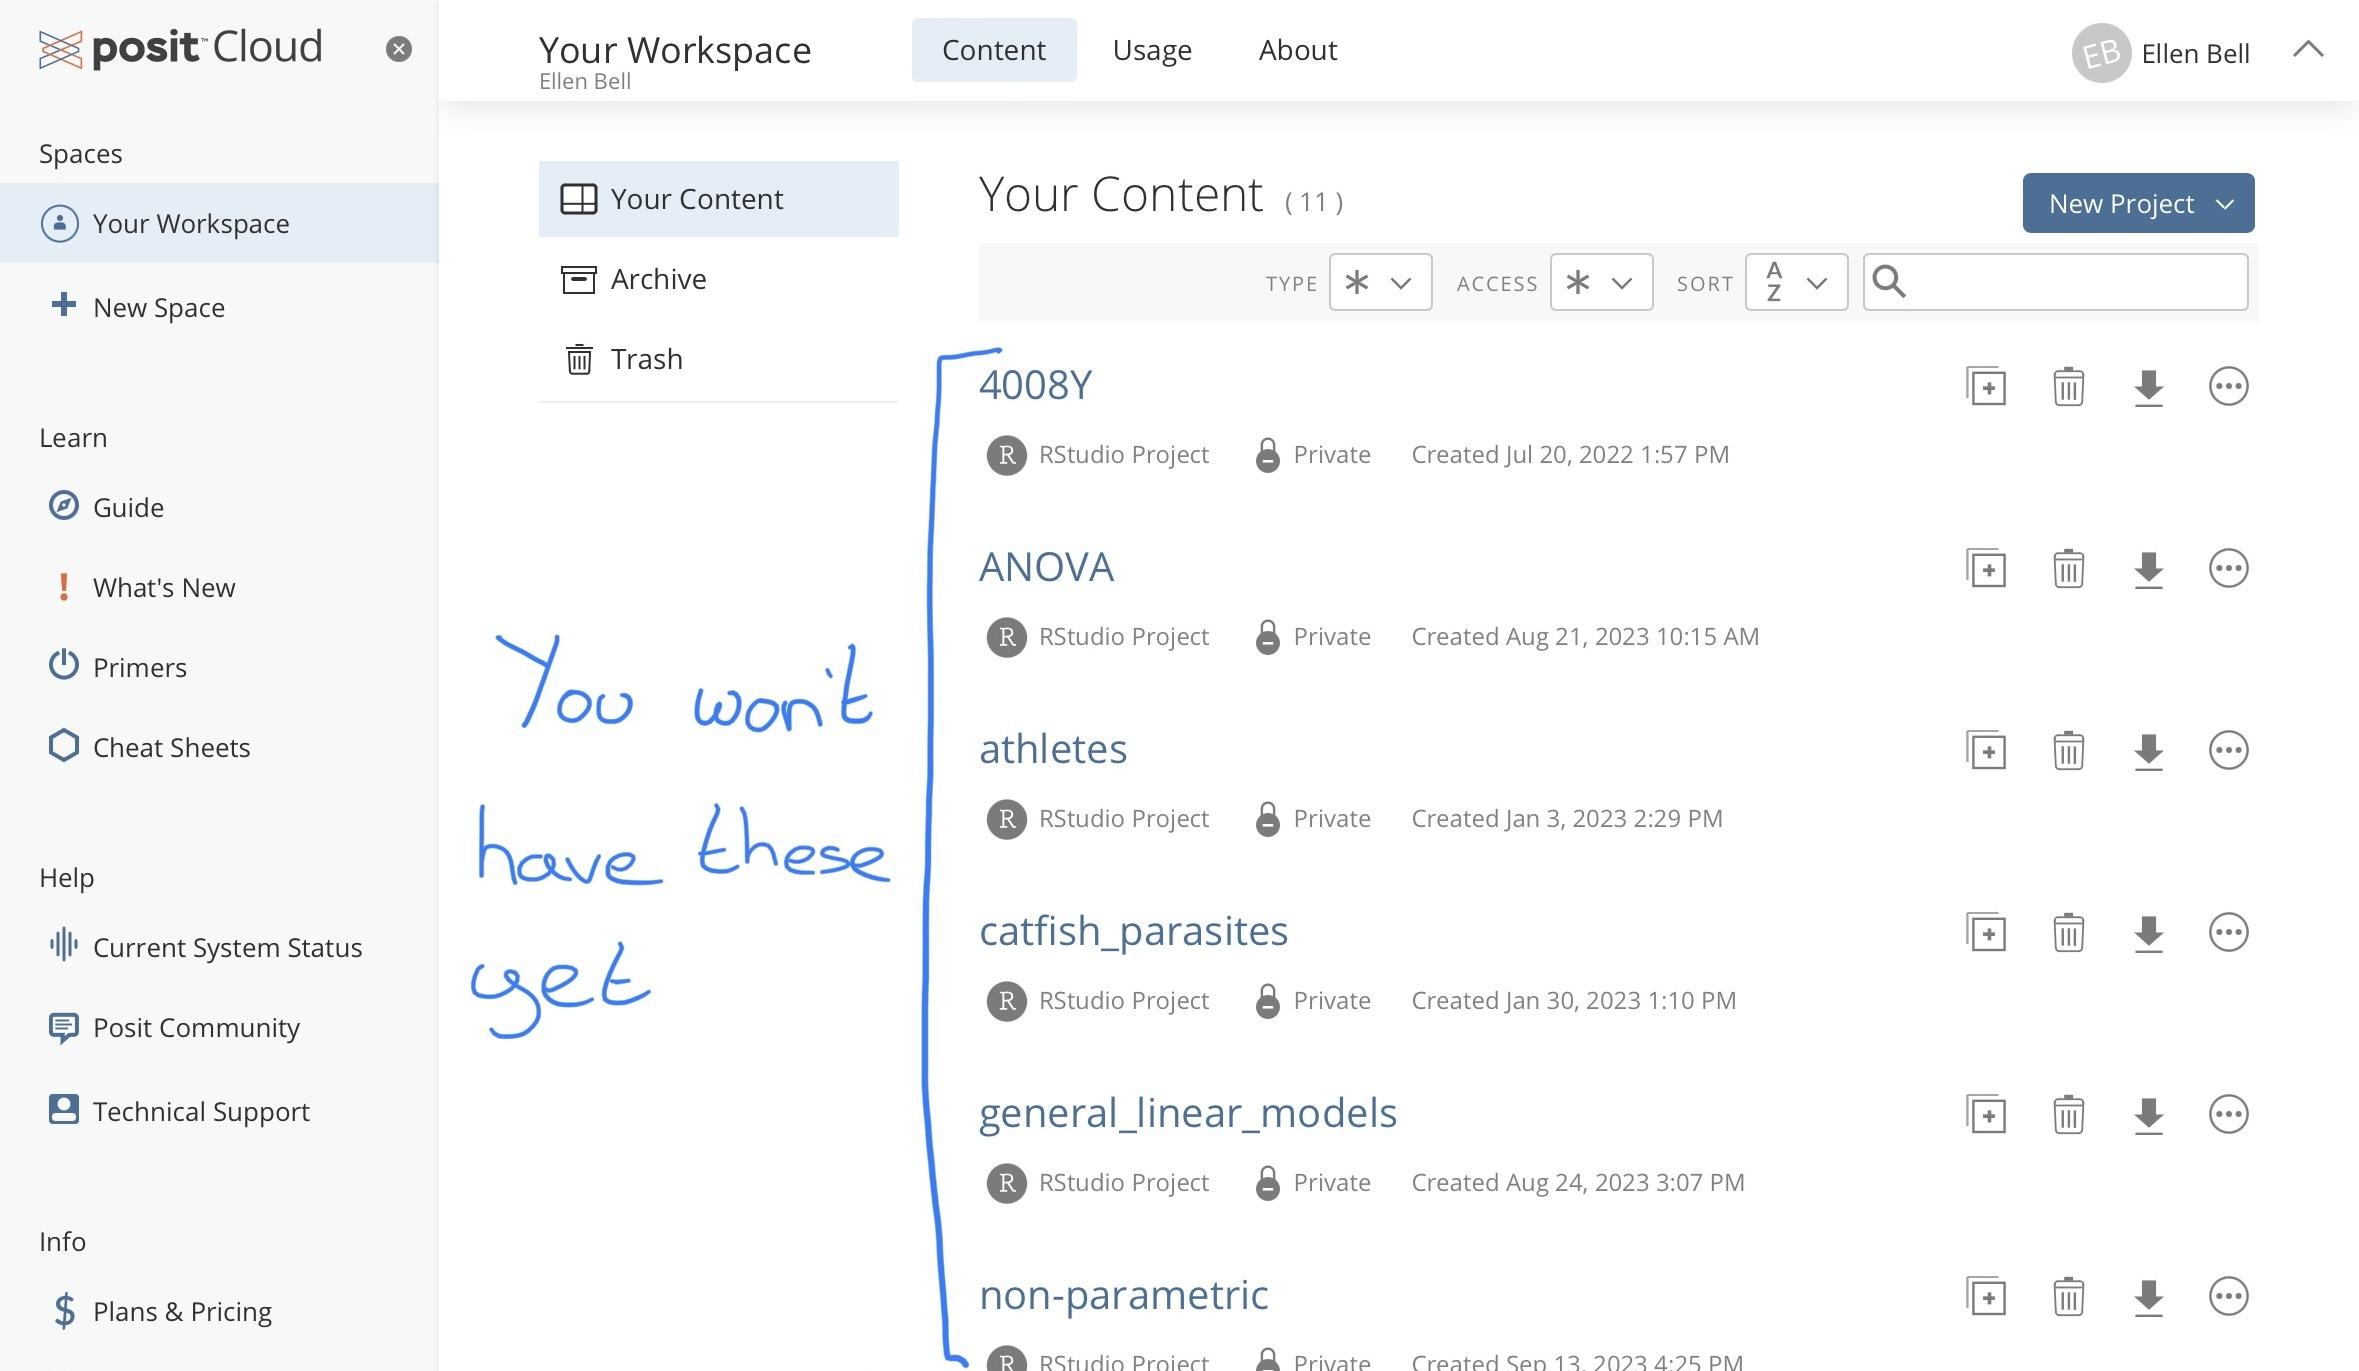
\includegraphics[width=0.9\linewidth]{figures/posit1} \caption{Your workspace in posit Cloud}\label{fig:unnamed-chunk-1}
\end{figure}

Under \textbf{Spaces} go to \textbf{Your Workspace} and under \textbf{Projects} create a \textbf{New Project \textgreater{} New R studio Project}.

\begin{figure}
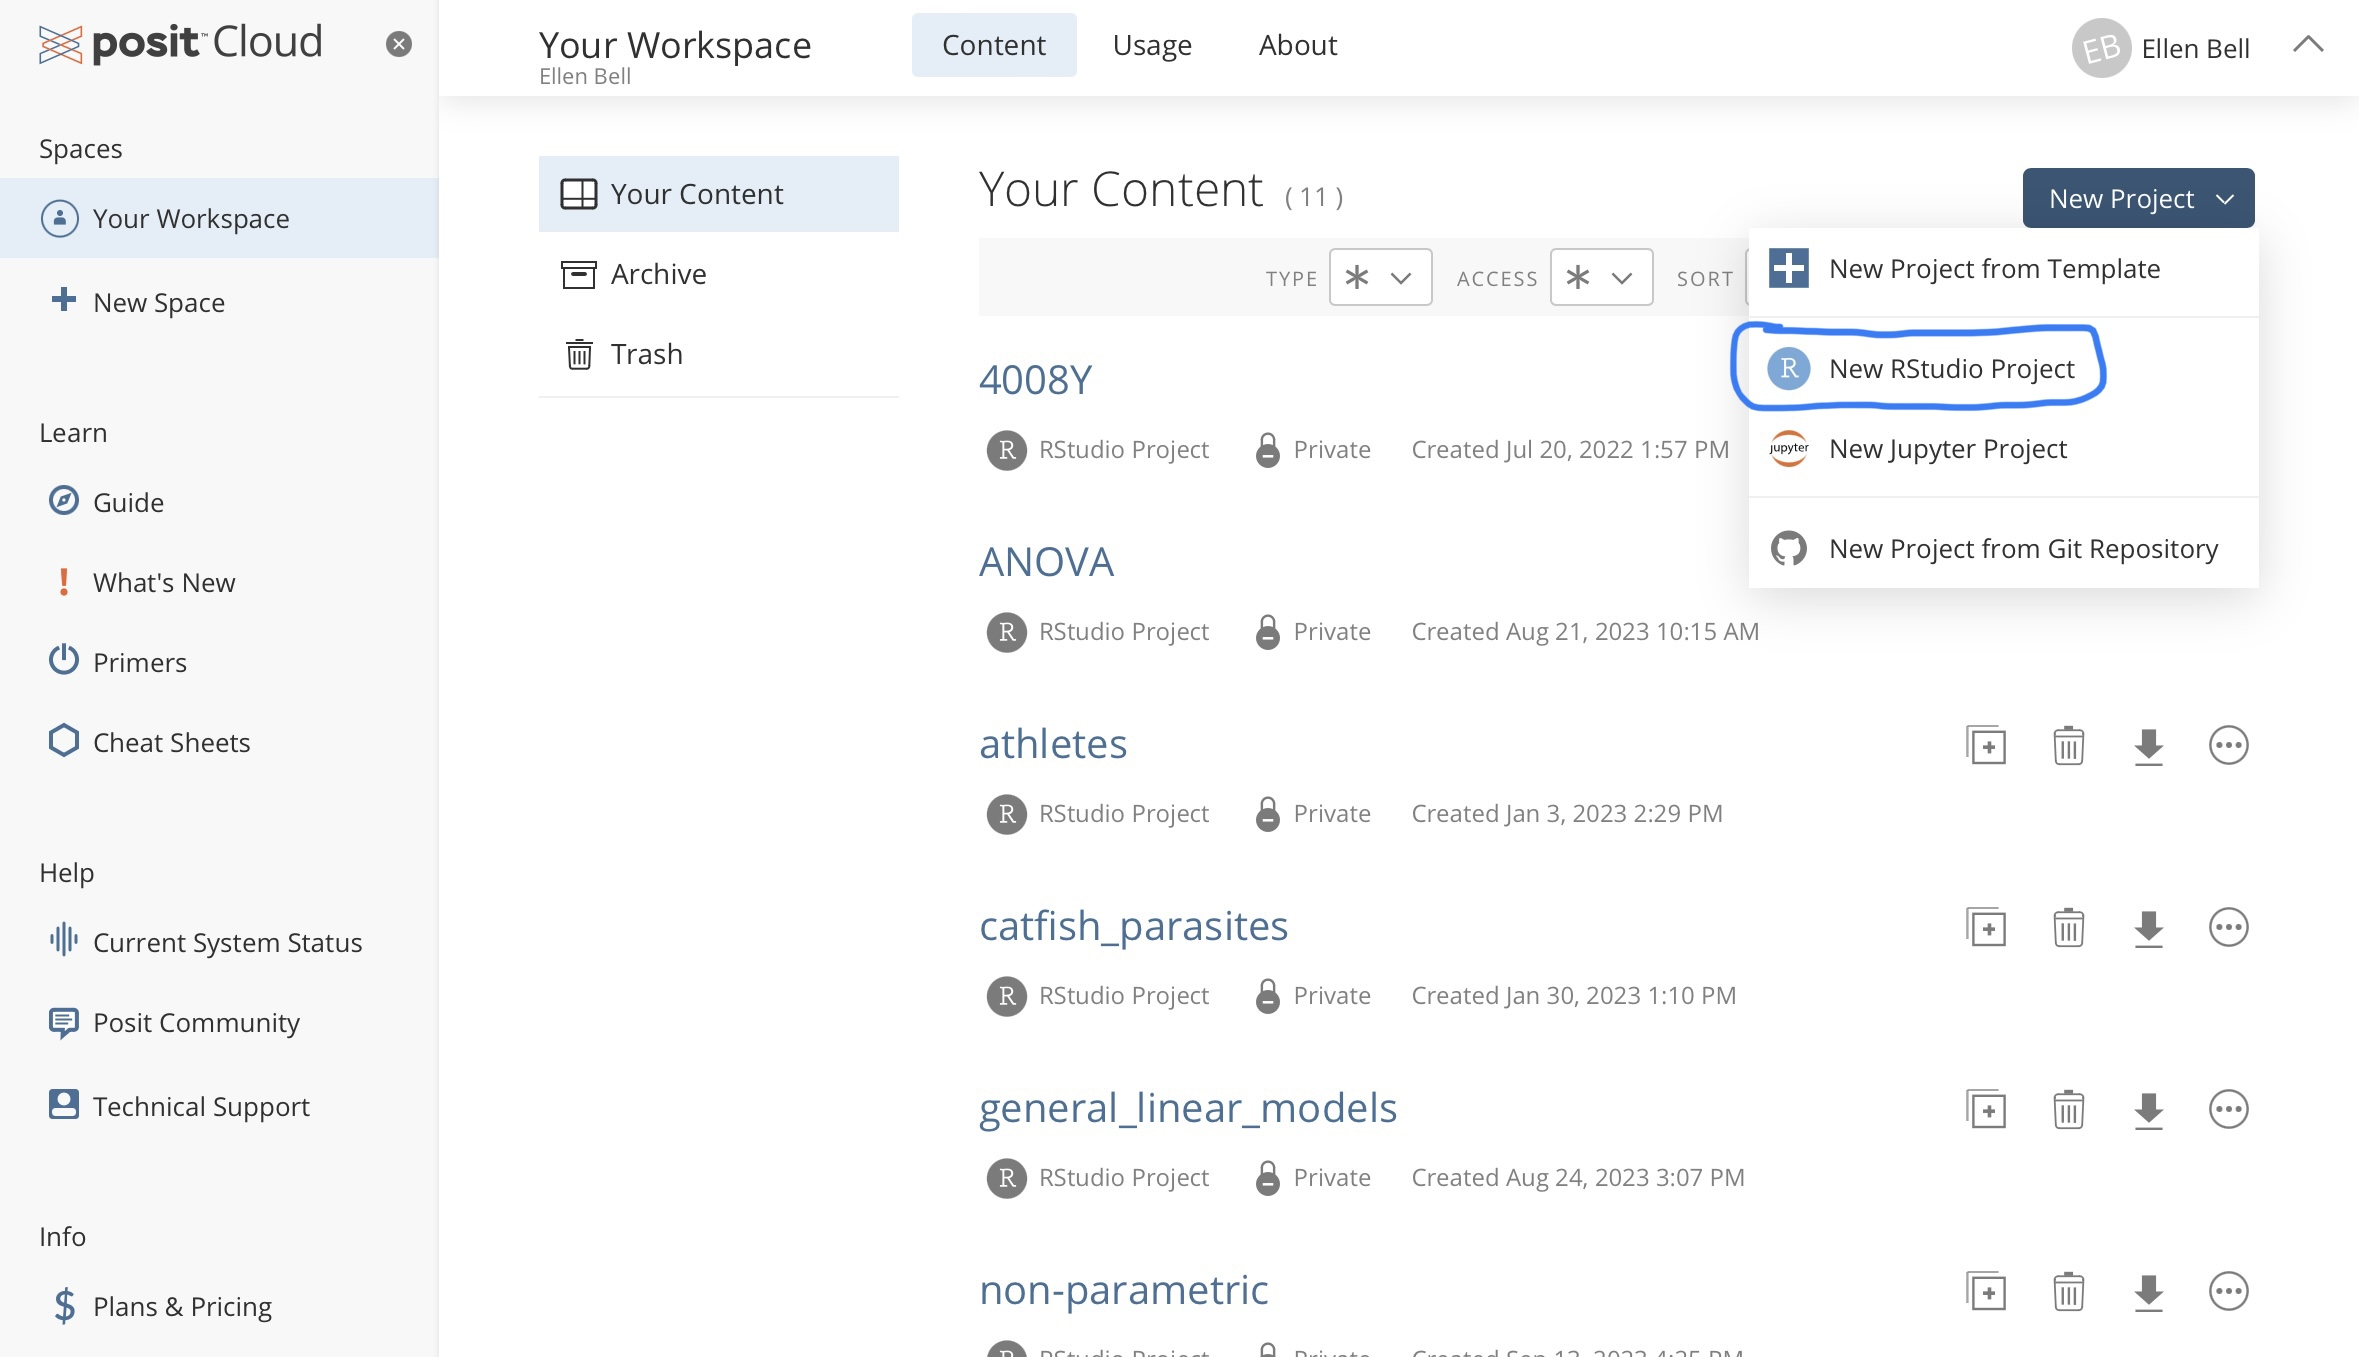
\includegraphics[width=0.9\linewidth]{figures/posit2} \caption{Creating a new project in posit Cloud}\label{fig:unnamed-chunk-2}
\end{figure}

Lets name this project \texttt{testing\_R}, notice that I have no spaces in my project name. Instead of a space I have used an underscore, there are a number of good habits you should try and adopt when naming projects or files and not including spaces is one of them, we will go over this in more depth in lectures and later chapters. You can rename your project by clicking on \textbf{Untitled Project} at the top of the window, and typing in your new project name.

\begin{figure}
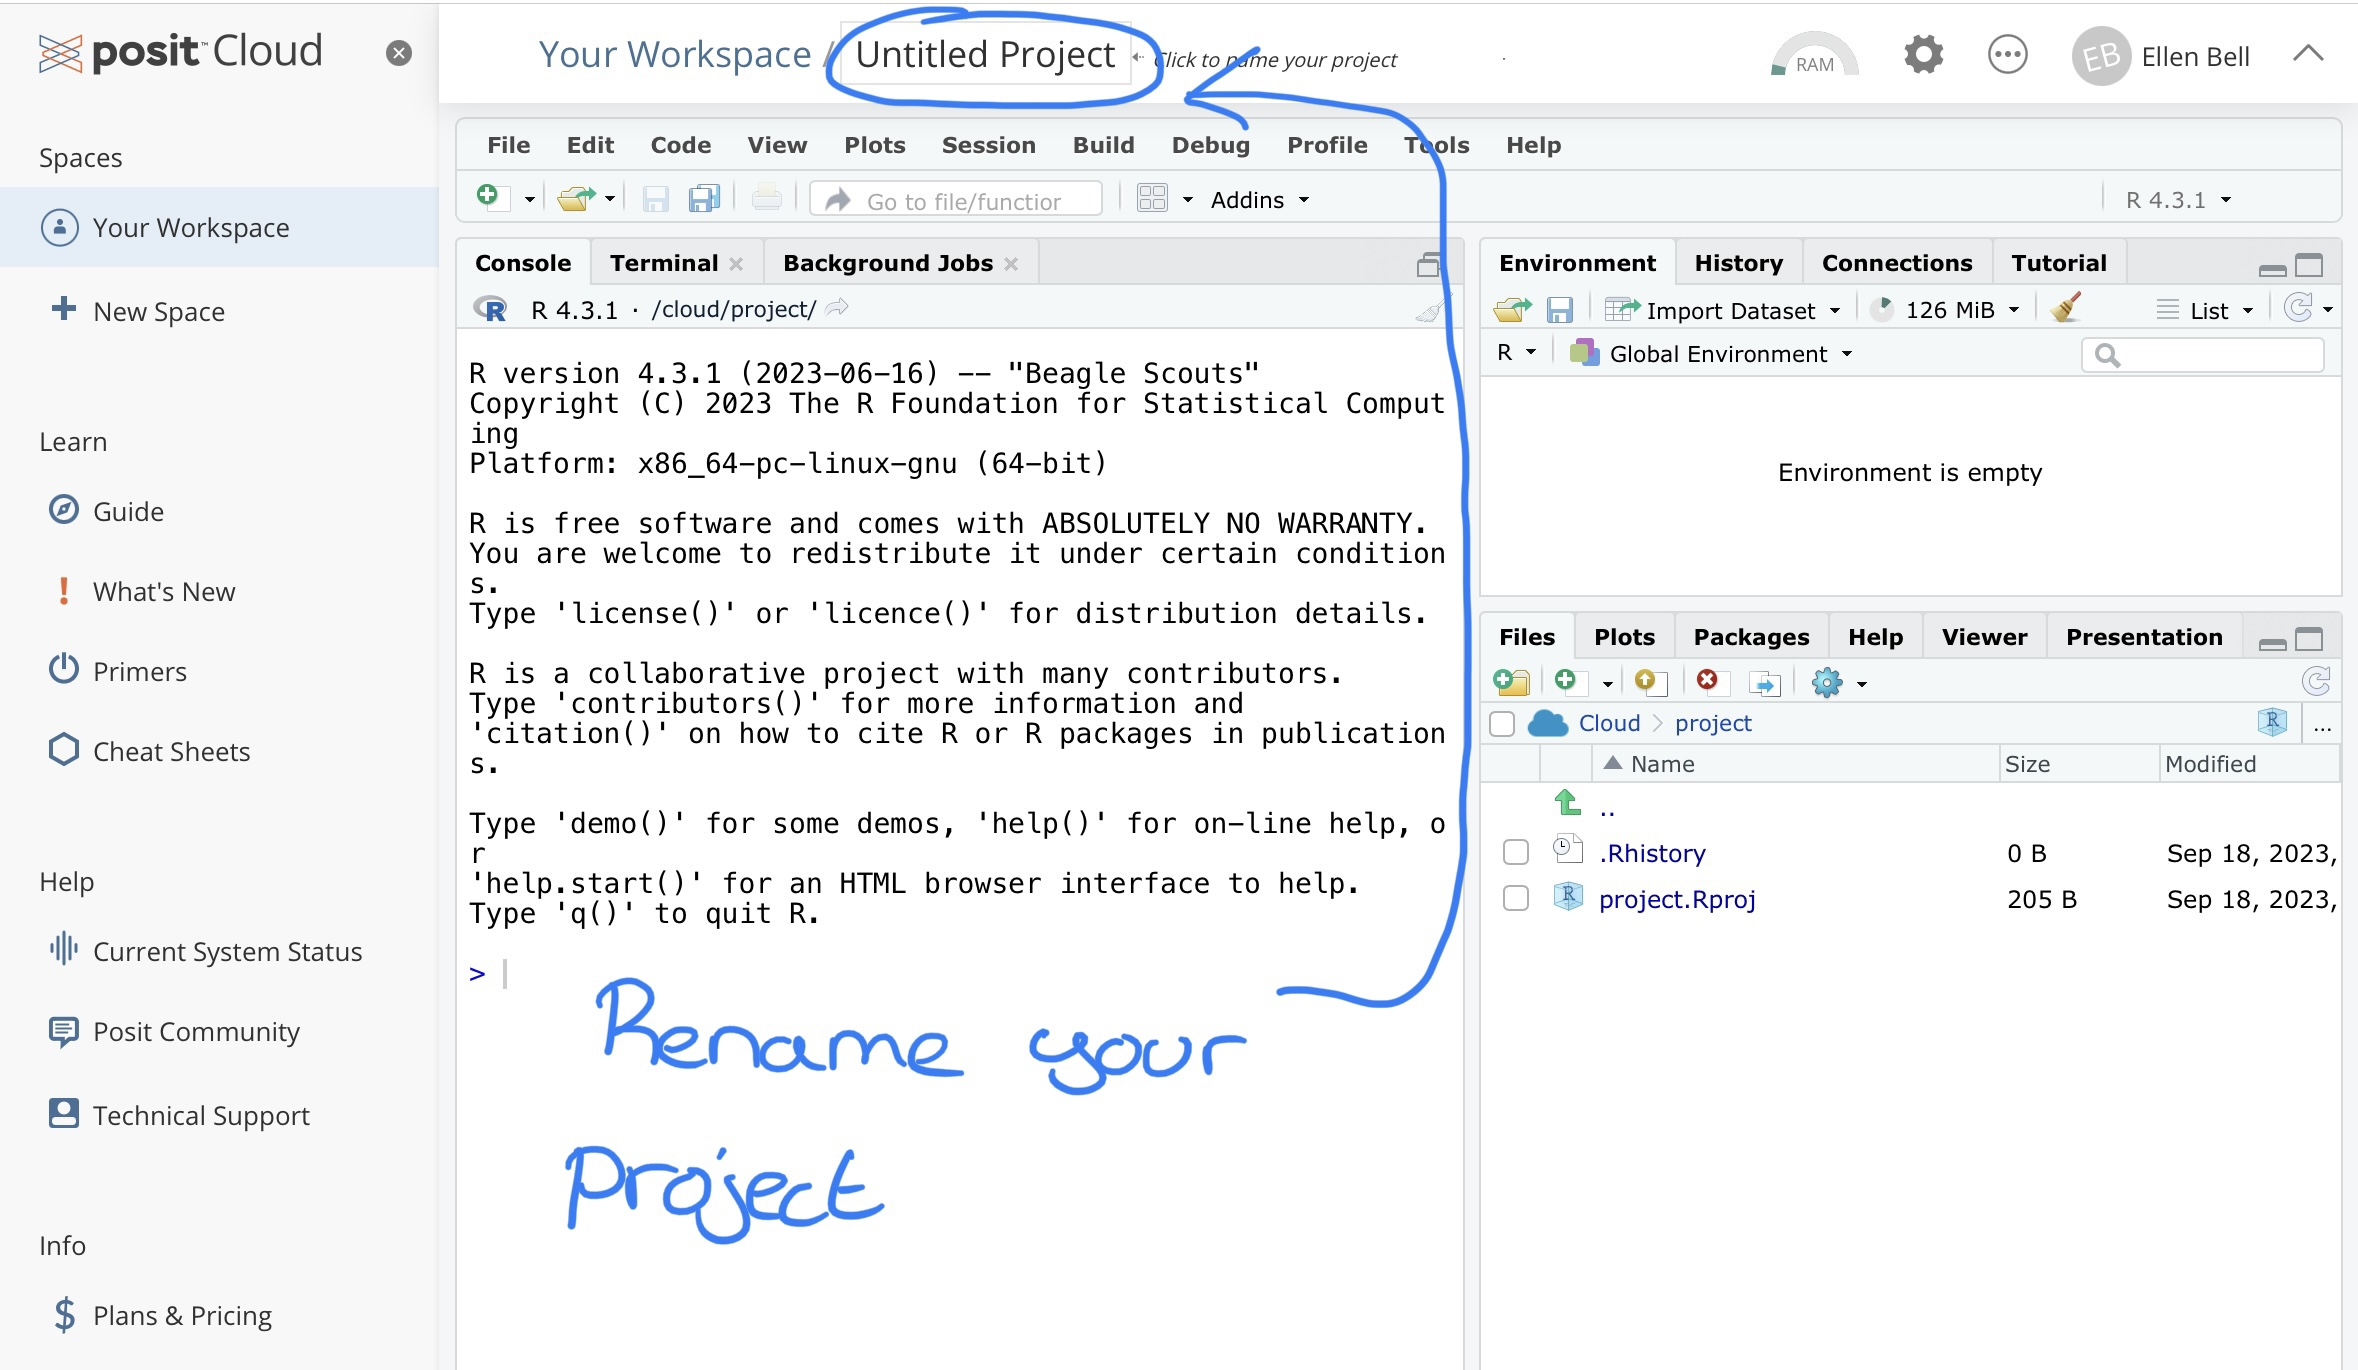
\includegraphics[width=0.9\linewidth]{figures/posit3} \caption{Renaming your project}\label{fig:unnamed-chunk-3}
\end{figure}

You will see that your new project has three panels with tabs showing the Console, Environment and Files for your project.

\begin{figure}
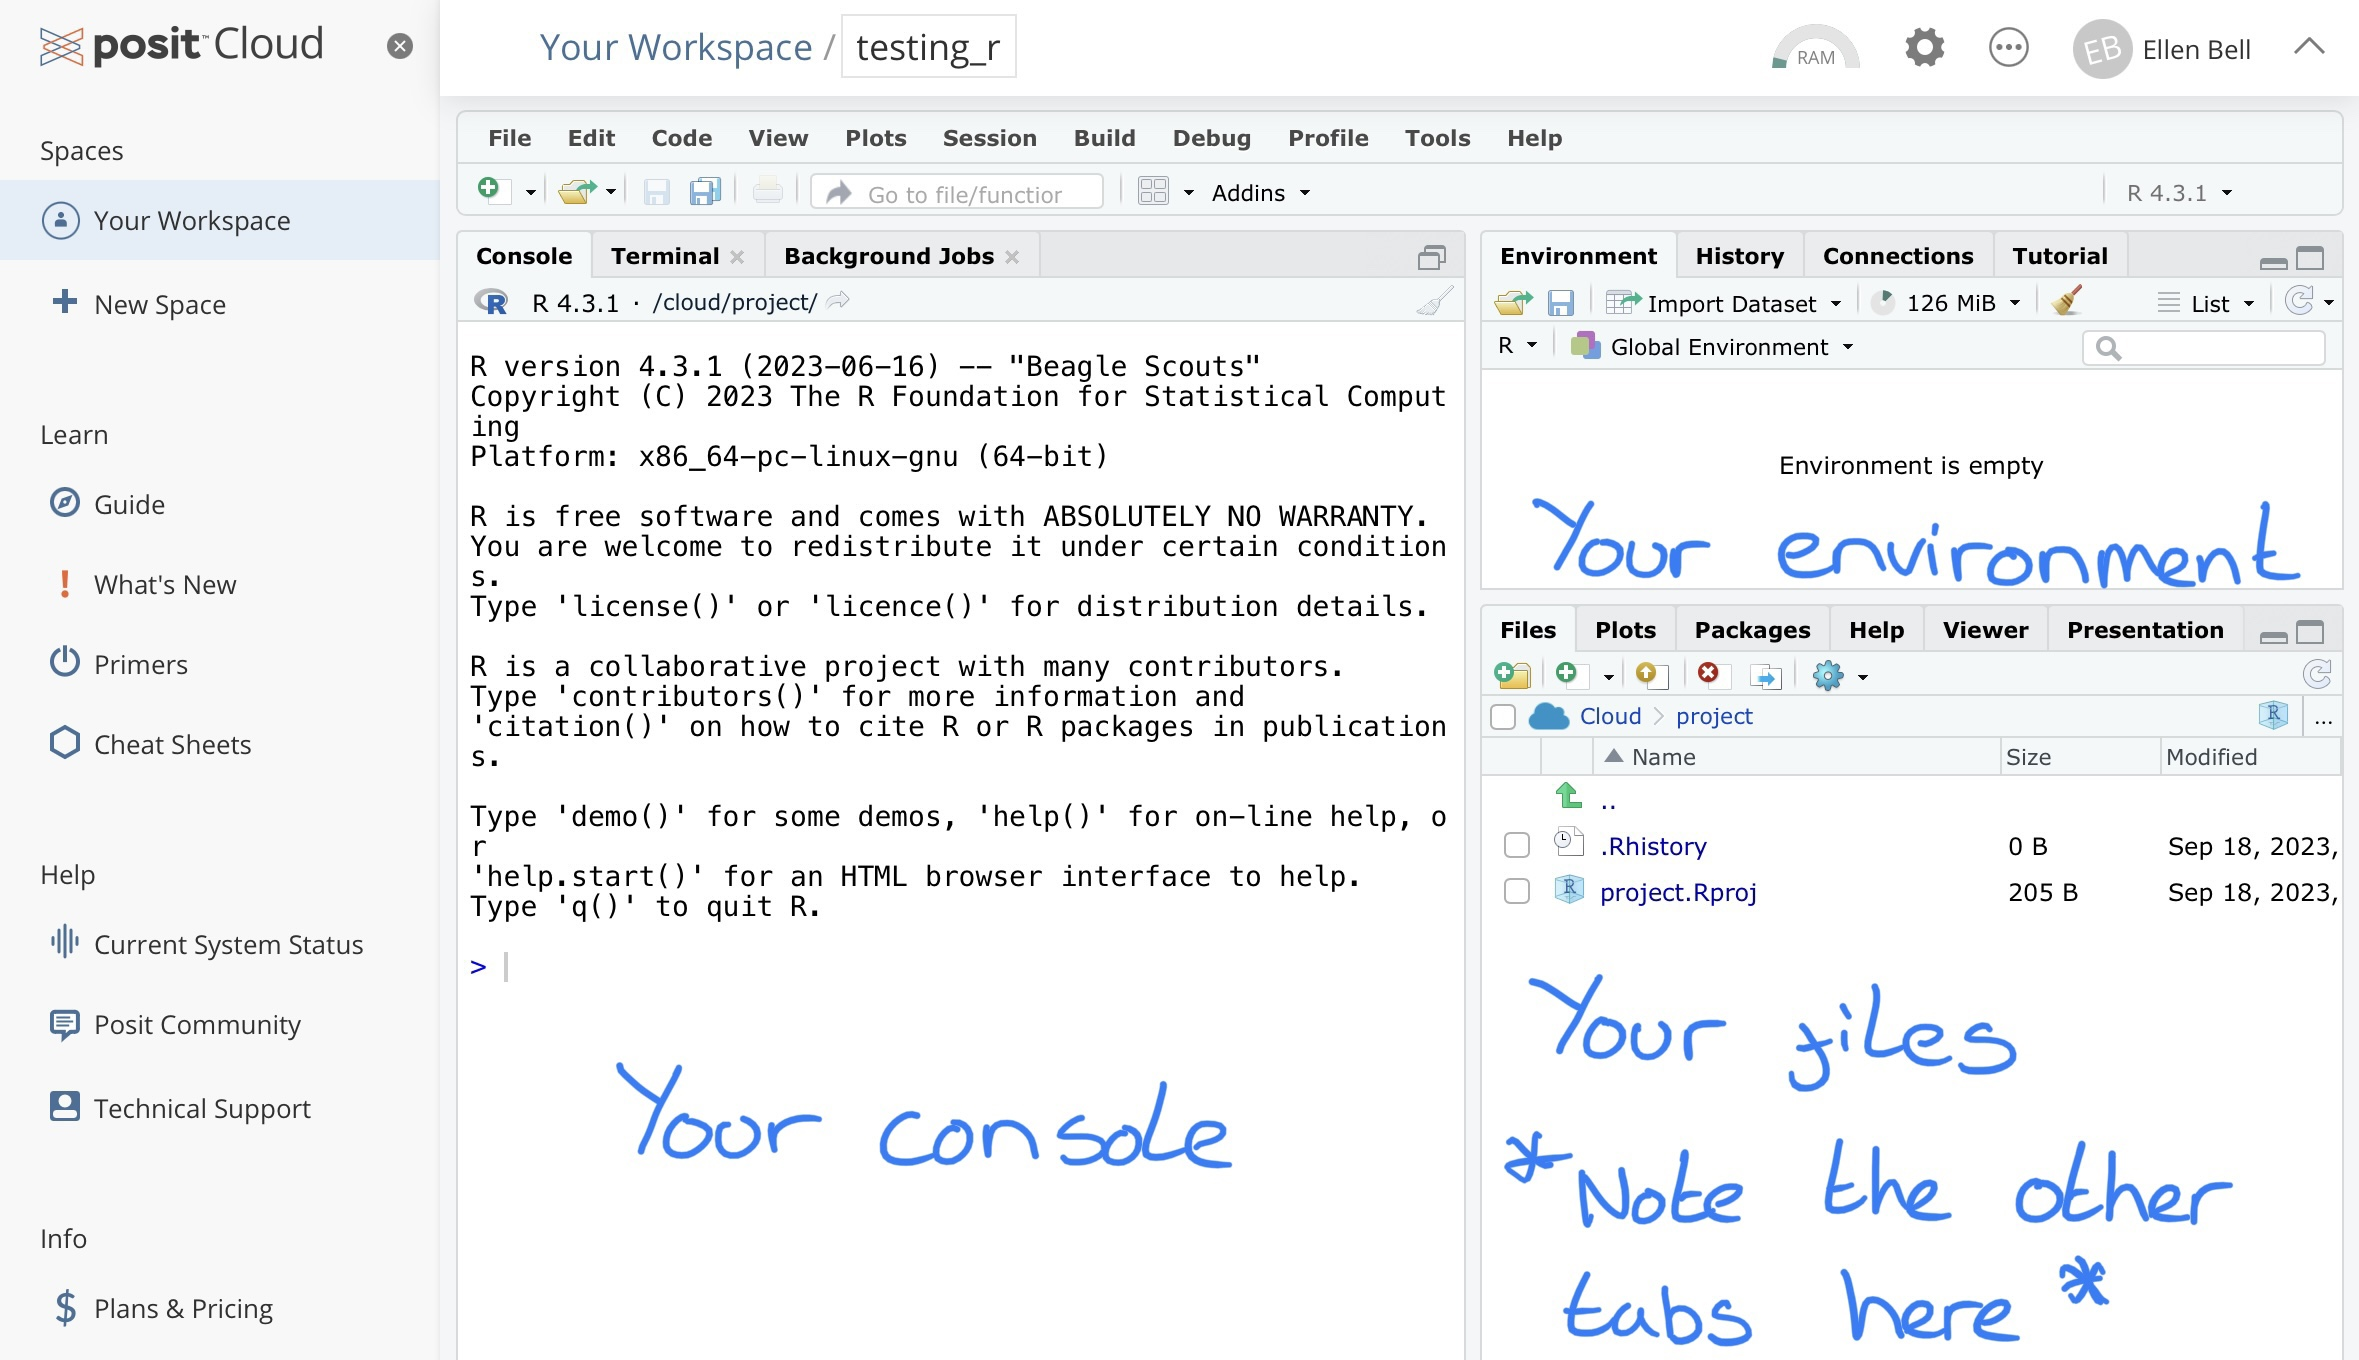
\includegraphics[width=0.9\linewidth]{figures/posit4} \caption{The three basic panels of an R Studio workspace}\label{fig:unnamed-chunk-4}
\end{figure}

\hypertarget{a-warning-on-managing-your-work-flow}{%
\subsection{A warning on managing your work flow}\label{a-warning-on-managing-your-work-flow}}

Your free posit Cloud account comes with some restrictions which you should be aware of. These are;

\begin{itemize}
\tightlist
\item
  You may have up to 50 projects in total
\item
  You are limited to 25 project hours per month
\item
  You have up to 1GB of RAM and 1 CPU per project
\end{itemize}

For the purposes of our work here these restrictions should not be a problem. But I strongly suggest you don't leave your coursework to the last minute. There are some options of last resort should this happen, you could install RStudio on your desktop for example, or you could open a new free posit Cloud account with a different email address and copy your script over. But with both of these options we run the risk of things getting complicated. Lets avoid that where we can! There are some ways you can increase the efficiency of your workspace which are documented below in Chapter \ref{efficiency}.

\hypertarget{efficiency}{%
\subsection{Maximising the efficiency of your workspace}\label{efficiency}}

We know there are limited project hours on our free posit Cloud accounts. But equally we will only be working with very small data sets, so we can tinker with resource usage. To reduce your resource usage. In your project, go to settings (the cogwheel sign), Resources, and drag all of the sliders down to the minimum setting, apply the changes, this will mean the project has to restart. This will mean that running the project for 1 hour will consume 0.5 project hours. We wont be doing anything particularly computationally intensive so there is no need for RAM of CPUs to be higher.

\begin{figure}
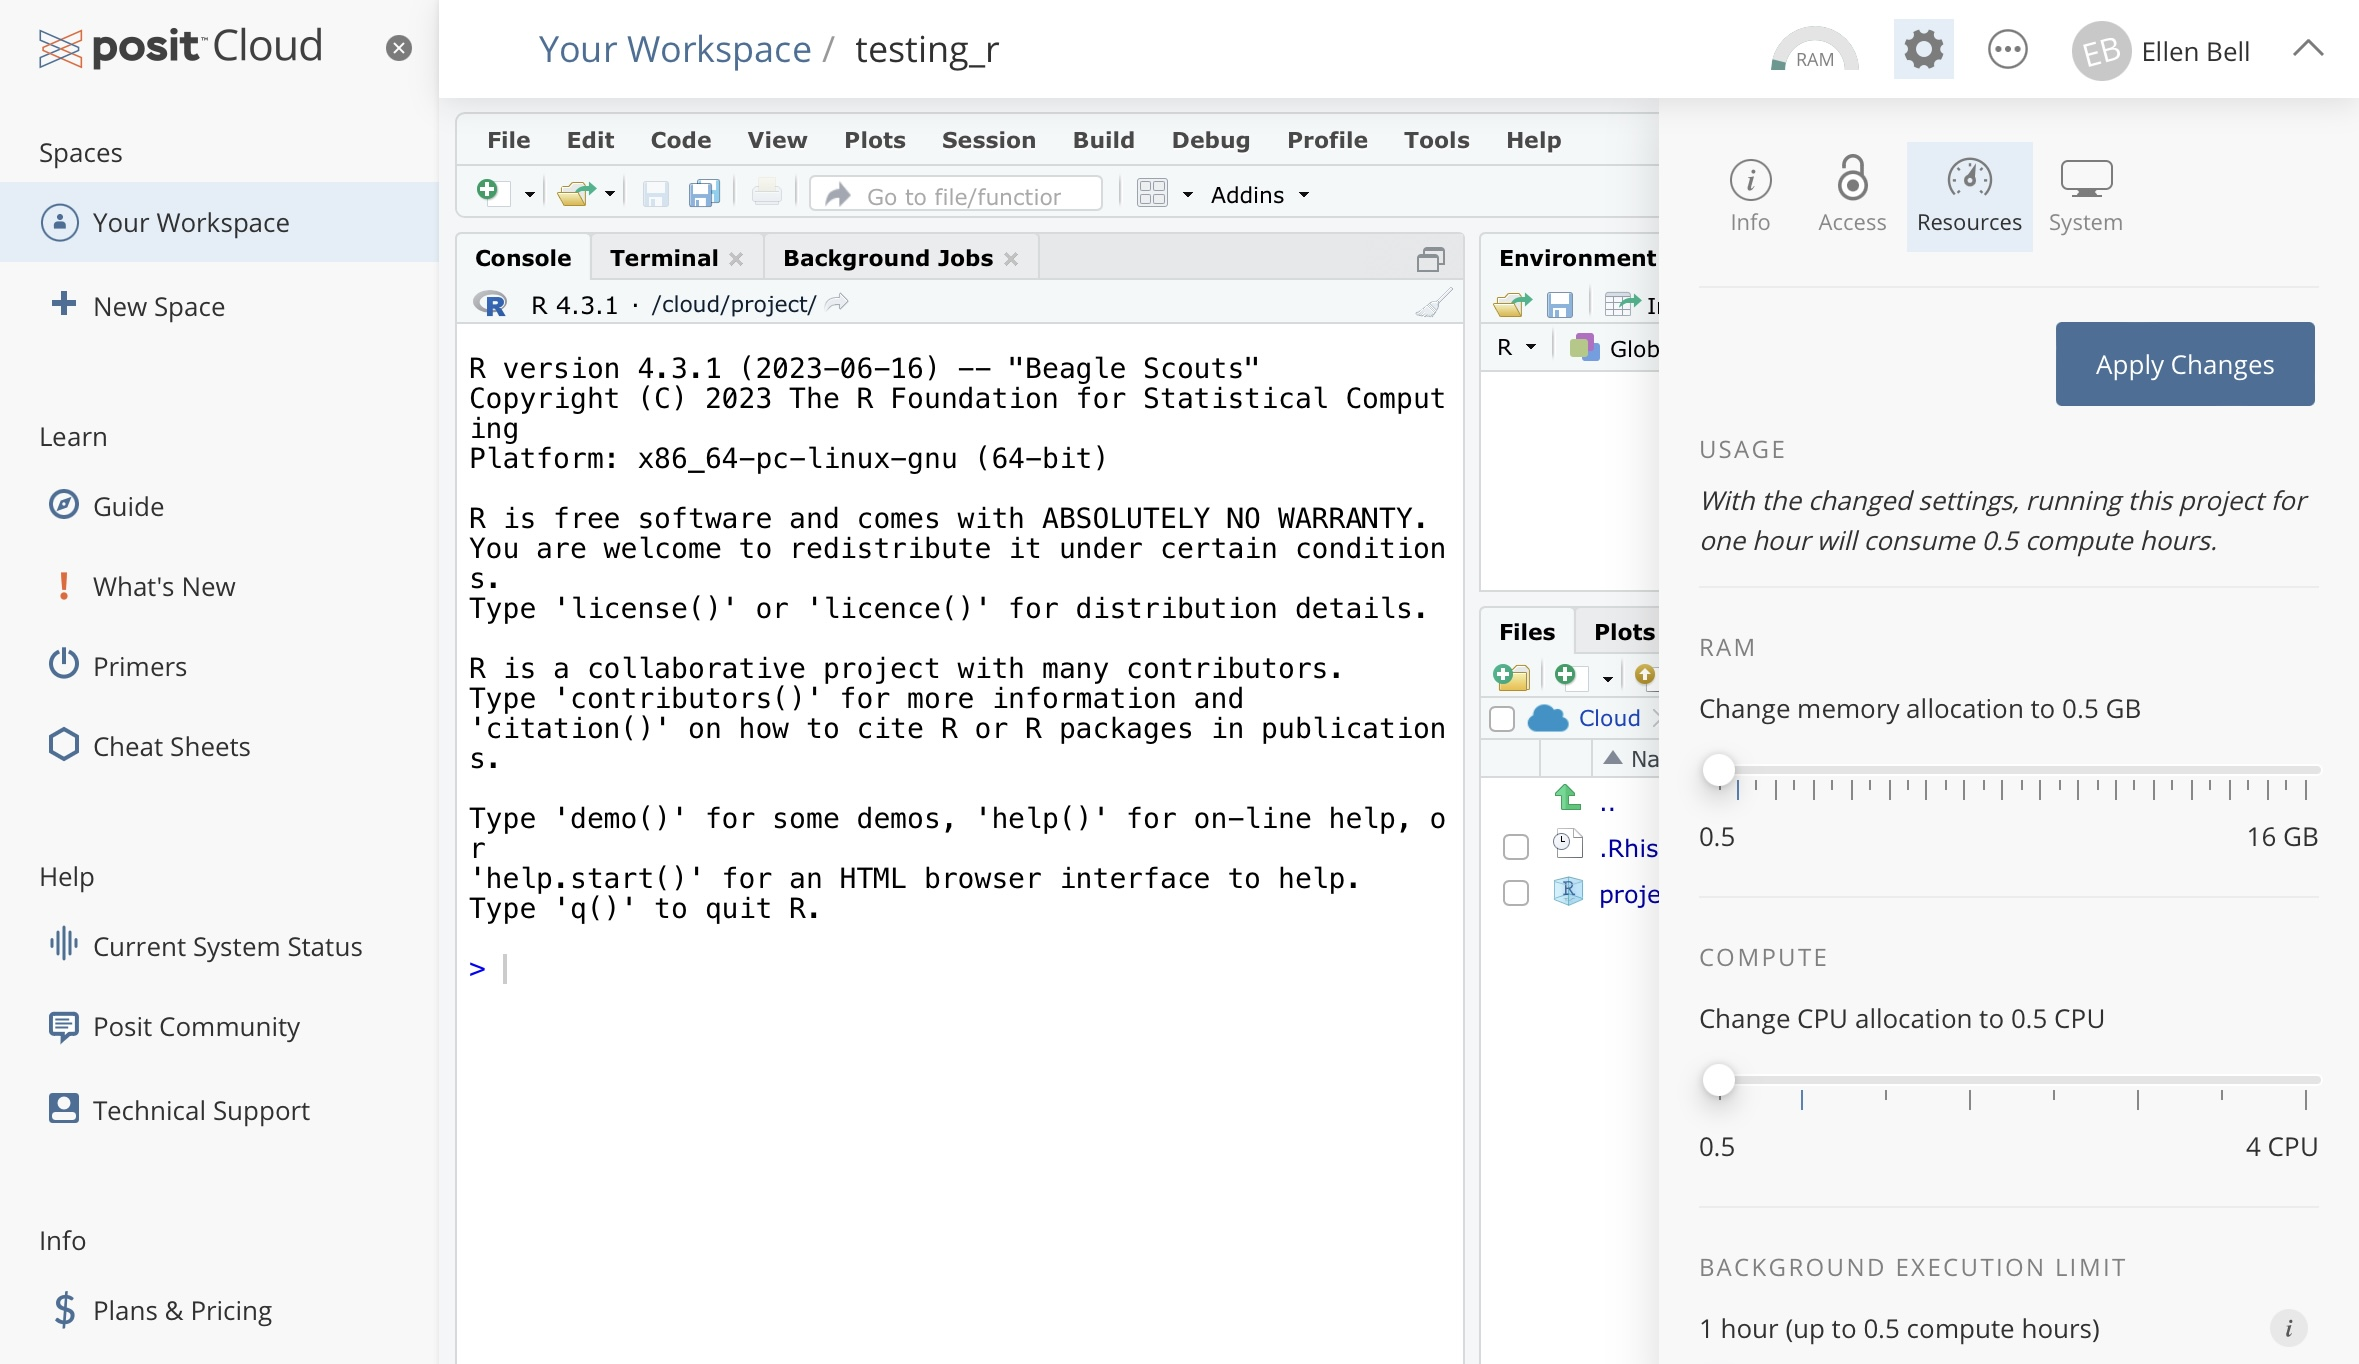
\includegraphics[width=0.9\linewidth]{figures/posit5} \caption{How to make your project more efficient}\label{fig:unnamed-chunk-5}
\end{figure}

\hypertarget{before-you-leave}{%
\section{Before you leave!}\label{before-you-leave}}

Log out of posit Cloud!

\hypertarget{c2}{%
\chapter{Some fundamentals to effective use of R}\label{c2}}

If you are already familiar with R this chapter will be a very swift refresher, you should still work through it though, it will also provide a good overview of posit Cloud.

Login to you posit Cloud account and go into your \texttt{testing\_R} project (see Chapter \ref{intro-to-posit} if you haven't done these steps yet)

\hypertarget{entering-commands-directly-into-the-console}{%
\section{Entering commands directly into the console}\label{entering-commands-directly-into-the-console}}

Lets start by playing with some commands in the console. Type or copy and paste the simple calculation (or command) shown below, into the console. Your text should appear next to the \texttt{\textgreater{}} symbol. Press \texttt{Enter} on your keyboard, this will instruct R to run the command.

\begin{Shaded}
\begin{Highlighting}[]
\DecValTok{5} \SpecialCharTok{+} \DecValTok{9}
\end{Highlighting}
\end{Shaded}

The two final lines of your output should look like this:

\begin{verbatim}
> 5 + 9
[1] 14
\end{verbatim}

So\ldots{} your initial command \texttt{5\ +\ 9} is shown after the \texttt{\textgreater{}}, symbol and the resulting output from R is shown after \texttt{{[}1{]}}. Don't worry too much about the syntax of \texttt{\textgreater{}} and \texttt{{[}1{]}} here. You can think of \texttt{\textgreater{}} as meaning that R is ready to receive a command and \texttt{{[}1{]}} as R telling you that the answer to the first part of your question is here (in this case \texttt{14}).

Try out some other commands\ldots{} What happens when you input the following?

\begin{Shaded}
\begin{Highlighting}[]
\DecValTok{362} \SpecialCharTok{*} \DecValTok{12}
\end{Highlighting}
\end{Shaded}

\begin{Shaded}
\begin{Highlighting}[]
\DecValTok{55} \SpecialCharTok{/} \DecValTok{5}
\end{Highlighting}
\end{Shaded}

\begin{Shaded}
\begin{Highlighting}[]
\NormalTok{(}\DecValTok{40} \SpecialCharTok{/} \DecValTok{990}\NormalTok{) }\SpecialCharTok{*} \DecValTok{100}
\end{Highlighting}
\end{Shaded}

\begin{Shaded}
\begin{Highlighting}[]
\DecValTok{4}\SpecialCharTok{\^{}}\DecValTok{2}
\end{Highlighting}
\end{Shaded}

See if you can work out what 30\% of 735 is using the R console

\hypertarget{using-an-r-script}{%
\section{Using an R script}\label{using-an-r-script}}

I have already mentioned the \textbf{reproducibility} factor as an advantage of using posit Cloud. This is because you can record and run all of your commands from an R script within posit Cloud. This means that you have a written record of your analysis workflow, what you did to your data at which stage, and you can do all of this without altering the original data files! This is super important because it means that if you revisit your work in a few weeks/months/years you can see exactly what you did AND if someone else needs to rerun any of your analysis or use your workflow on some other data, they can!

So lets go about setting up your new script. You currently have three panels in posit Cloud. If you go to \textbf{file \textgreater{} New File \textgreater{} R Script} a new panel will open.

\begin{figure}
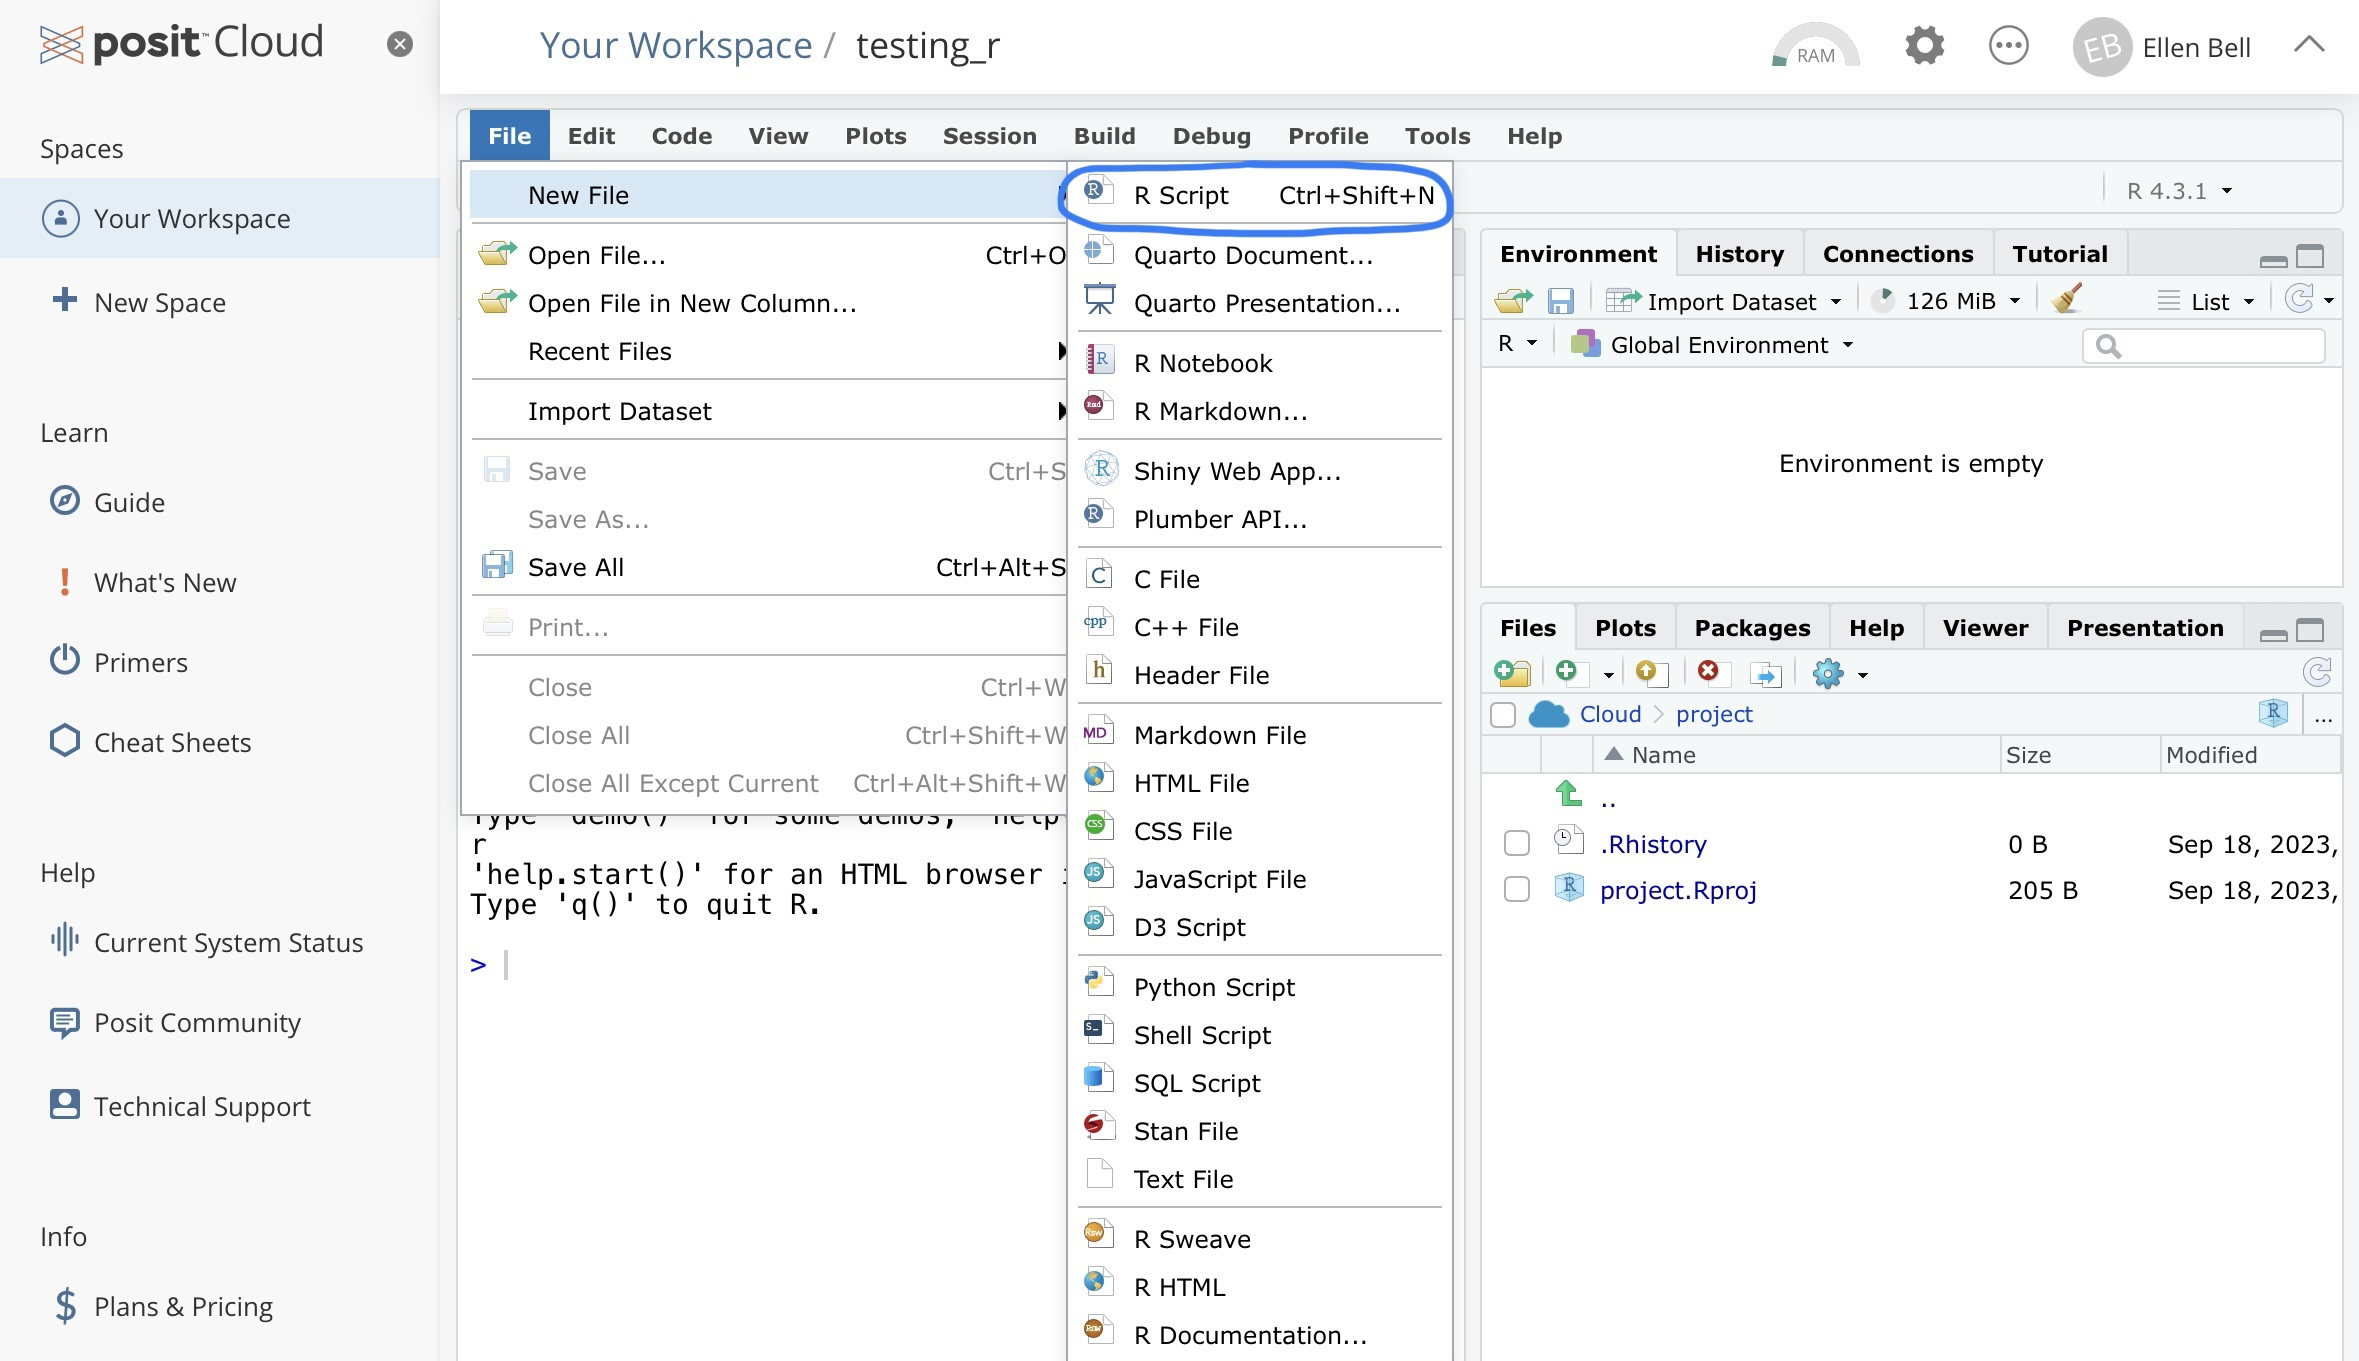
\includegraphics[width=0.9\linewidth]{figures/posit6} \caption{How to create a new R script}\label{fig:unnamed-chunk-11}
\end{figure}

\begin{figure}
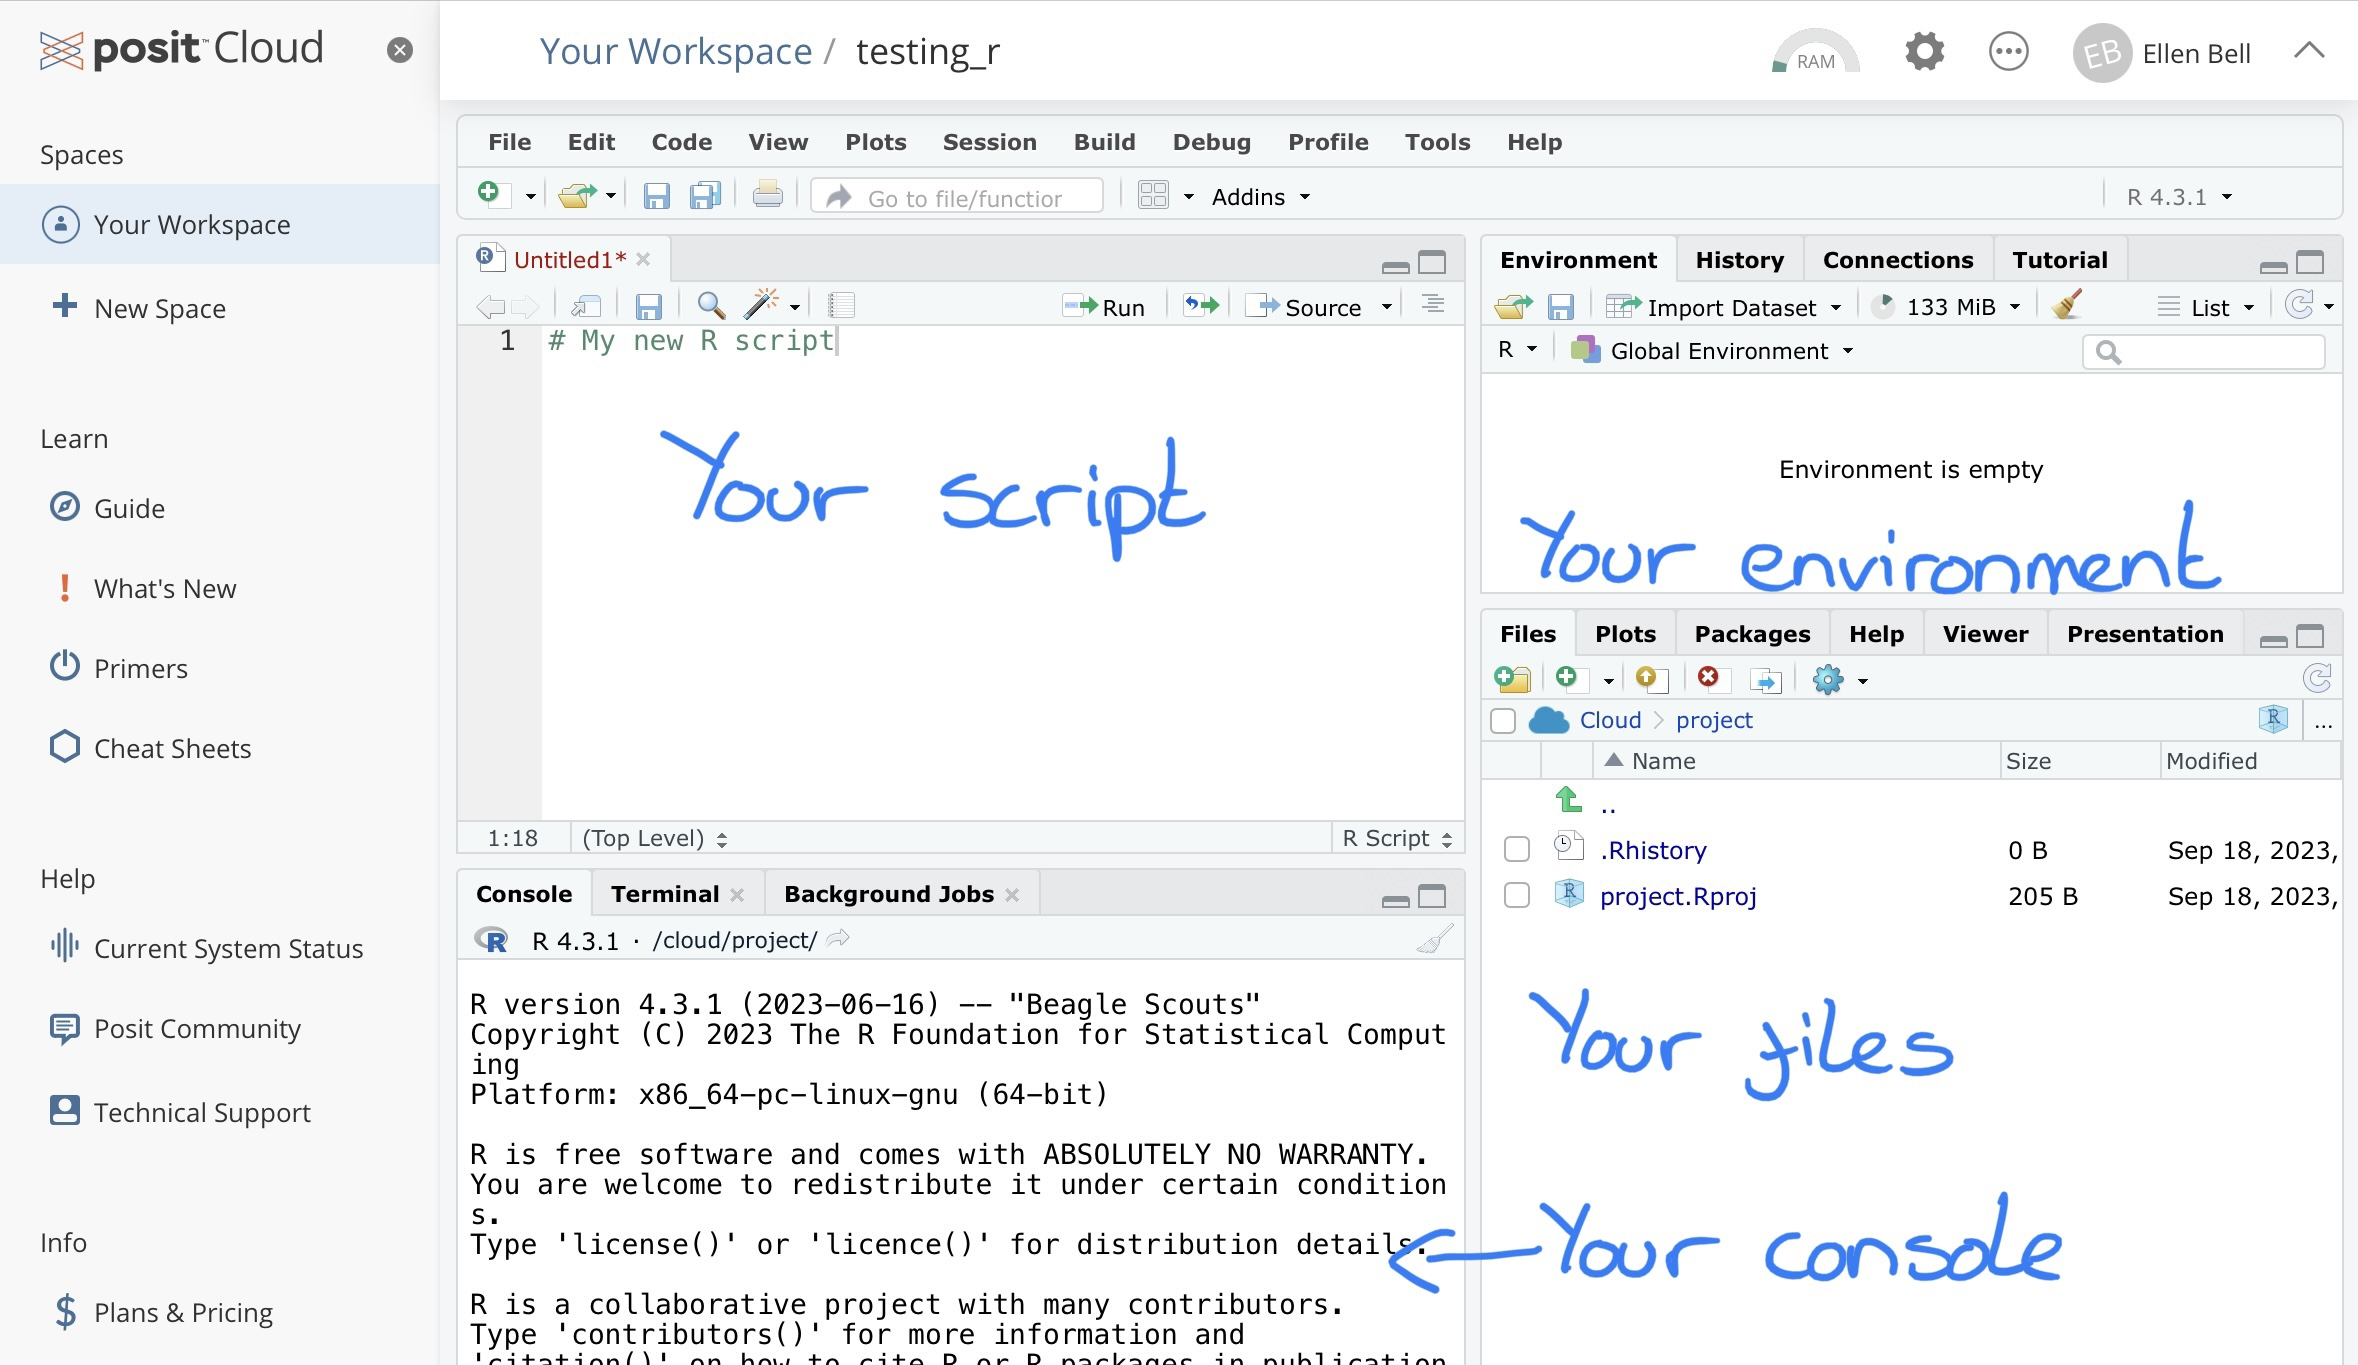
\includegraphics[width=0.9\linewidth]{figures/posit7} \caption{The four panels of an R Studio workspace}\label{fig:unnamed-chunk-12}
\end{figure}

This new panel is essentially a text file where you can write your commands into a script and then send them down to the console when you want to run them. Lets have a play. Copy the below into your new R script.

\begin{Shaded}
\begin{Highlighting}[]
\DecValTok{362} \SpecialCharTok{*} \DecValTok{12}

\DecValTok{55} \SpecialCharTok{/} \DecValTok{5}

\NormalTok{(}\DecValTok{40} \SpecialCharTok{/} \DecValTok{990}\NormalTok{) }\SpecialCharTok{*} \DecValTok{100}

\DecValTok{4}\SpecialCharTok{\^{}}\DecValTok{2}
\end{Highlighting}
\end{Shaded}

These are all commands you have run before but now if you save your script you will have a text based document with your progress saved. It doesn't make a huge amount of sense to do this now because these are just a un-associated set of calculations and we are just playing with the interface, but you could if you wanted to.

Ok, so now we are ready to execute our commands. You can do this with each calculation individually, line by line, or you can run the whole script.

To run your script line by line, place your cursor on the line you wish to run and you can either;

\begin{itemize}
\tightlist
\item
  Click on the \textbf{Run} button on the top right of the script panel
\item
  Press \textbf{ctrl + Enter} (or \textbf{Command + Enter} on mac)
\end{itemize}

Or if you wish to run the entire script you can either;

\begin{itemize}
\tightlist
\item
  Manually highlight the script and click the \textbf{Run} button or press \textbf{ctrl + Enter} (or \textbf{Command + Enter} on mac)
\item
  Press \textbf{ctrl + A} (or \textbf{Command + A} on mac) and then click the run button or press \textbf{ctrl + Enter} (or \textbf{Command + Enter} on mac)
\end{itemize}

\hypertarget{creating-objects}{%
\section{Creating objects}\label{creating-objects}}

As we have just seen, R can be used to perform calculations. However, we can use R to perform tasks that are much more complex. In order to do this we are going to have to learn about objects.

Create a new R script in your current and save it under the name \texttt{objects}. You should see it appear as \texttt{object.R} under the \textbf{Files} tab in the bottom right panel. Run the following command using your script.

\begin{Shaded}
\begin{Highlighting}[]
\NormalTok{A }\OtherTok{\textless{}{-}} \DecValTok{50}
\end{Highlighting}
\end{Shaded}

What you have essentially done here, is told R to create an object called \texttt{A} and to store the number \texttt{50} inside it using the syntax \texttt{\textless{}-}. After running the command you should see your object \texttt{A} and \texttt{50} pop up under \textbf{Environment} and \textbf{Values} in the top right hand panel, so you can see that \texttt{50} has been stored in \texttt{A}.

Lets create some more objects;

\begin{Shaded}
\begin{Highlighting}[]
\NormalTok{B }\OtherTok{\textless{}{-}} \DecValTok{6}
\end{Highlighting}
\end{Shaded}

Now see what happens if you run the following command;

\begin{Shaded}
\begin{Highlighting}[]
\NormalTok{A }\SpecialCharTok{*}\NormalTok{ b}
\end{Highlighting}
\end{Shaded}

Oh dear\ldots{} we have an error\ldots{}

\begin{verbatim}
> A * b
Error: object 'b' not found
\end{verbatim}

This is because R has absolutely no flexibility with typos. It is looking for an object called \texttt{b} when there is no object called \texttt{b} in your environment. There is an object called \texttt{B}, but to R, \texttt{B} and \texttt{b} are completely different things. Try running this instead;

\begin{Shaded}
\begin{Highlighting}[]
\NormalTok{A }\SpecialCharTok{*}\NormalTok{ B}
\end{Highlighting}
\end{Shaded}

Hopefully you should now have an output that looks like this

\begin{verbatim}
> A * B
[1] 300
\end{verbatim}

This is a very simple example. But lets try to demonstrate why saving values within objects may be useful. Lets say you are interested in looking at the number of students who get freshers flu in Week 1 of teaching at UEA. You have a class size of 200 students and 15 of them report that they have contracted freshers flu. Use the following script to calculate the percentage of students with freshers flu.

\begin{Shaded}
\begin{Highlighting}[]
\CommentTok{\# Create two objects, one for your total class and one for those that have flu}
\CommentTok{\# Notice that neither of my object names contain spaces}
\CommentTok{\# If you need a space always use an underscore or full stop}
\NormalTok{total\_class }\OtherTok{\textless{}{-}} \DecValTok{200}
\NormalTok{with\_flu }\OtherTok{\textless{}{-}} \DecValTok{15}

\CommentTok{\# Calculate the percentage of students with flu in week 1}
\NormalTok{percentage\_with\_flu }\OtherTok{\textless{}{-}}\NormalTok{ (with\_flu}\SpecialCharTok{/}\NormalTok{total\_class)}\SpecialCharTok{*}\DecValTok{100}
\end{Highlighting}
\end{Shaded}

If you look in your Environment in the top right panel you should see the percentage of students with flu calculated and stored under \texttt{percentage\_with\_flu}. You can use the following command to see it printed in the console.

\begin{Shaded}
\begin{Highlighting}[]
\FunctionTok{print}\NormalTok{(percentage\_with\_flu)}
\end{Highlighting}
\end{Shaded}

Some students have been late in reporting their symptoms. A week later you hear that \texttt{7} more students also had freshers flu in Week 1. If you had been typing into the console and not using objects you would have to type this script out all over again. But you don't need to. You just need to change your entry for \texttt{with\_flu} from \texttt{15} to \texttt{22}. Do that now and re-run the script. By editing the \texttt{15}, R will overwrite the object \texttt{with\_flu} to represent the new value of \texttt{22}. If you run the last line of code then the percentage of students with flu will also update.

This may seem like a very simple example, and it is, but we are still building up your knowledge of R so you will have to take my word for it that objects will be very helpful to you as we progress :). You will also see, that objects can contain a range of different types of data. We will cover some of these in lectures, but for now lets leave objects and have a think about functions and packages.

\hypertarget{what-are-functions-and-packages}{%
\section{What are functions and packages?}\label{what-are-functions-and-packages}}

If you have the coding skills it is possible to do pretty much whatever you like with your data in R. However, why reinvent the wheel trying to write your own complex scripts, when a lot of very clever coders have already written lots of functional bits of code, known as \textbf{functions}, for general use. Functions can be thought of as a piece of code that is designed to perform a set task. R comes with lots of functions already built in, but there are also lots of additional functions that are stored in \textbf{packages}.

Packages are containers that can hold sets of functions or data and as the course progresses you will use a range of packages that contain useful functions and data. For example the data visualisation package (which you will become very familiar with later on) \texttt{ggplot2} contains ranges of functions which allow you to define how your plot or graph will look, for example \texttt{geom\_bar} is a function within the \texttt{ggplot2} package that contains the instructions required to build a bar chart.

\hypertarget{using-functions}{%
\subsection{Using functions}\label{using-functions}}

We actually have already had some exposure to functions. You used the print function earlier when you asked R to print out the value contained within the \texttt{percentage\_with\_flu} object. But lets have a go at using another function.

\begin{Shaded}
\begin{Highlighting}[]
\CommentTok{\# First of all we need some data}
\CommentTok{\# Notice the syntax, by using c() I have told R to prepare for a list of values}
\CommentTok{\# Each value is separated by a comma}
\NormalTok{data }\OtherTok{\textless{}{-}} \FunctionTok{c}\NormalTok{(}\DecValTok{2}\NormalTok{,}\DecValTok{4}\NormalTok{,}\DecValTok{6}\NormalTok{,}\DecValTok{8}\NormalTok{,}\DecValTok{10}\NormalTok{,}\DecValTok{12}\NormalTok{,}\DecValTok{14}\NormalTok{,}\DecValTok{16}\NormalTok{,}\DecValTok{18}\NormalTok{,}\DecValTok{20}\NormalTok{)}

\CommentTok{\# Now I want to know what the total value of data is if I add all the values stored within it together}
\NormalTok{total }\OtherTok{\textless{}{-}} \FunctionTok{sum}\NormalTok{(data)}
\end{Highlighting}
\end{Shaded}

In the above piece of code we have created some data, as a list of values, and stored them under the object name data. We have then used the function \texttt{sum()}. We have essentially told R that we wish it to perform the function \texttt{sum()} on everything contained within the object \texttt{data} and store it in another object called \texttt{total}. You can see the value within \texttt{total} in your environment, can you work out how to get R to print the value of \texttt{total} out?

If you ever need help working out how to use a function you can use another function \texttt{help()}. Try inputing the code below into your console.

\begin{Shaded}
\begin{Highlighting}[]
\FunctionTok{help}\NormalTok{(sum)}
\end{Highlighting}
\end{Shaded}

This should bring up a help file in your bottom right hand panel that describes and explains the use of the function \texttt{sum()}.

\hypertarget{installing-packages}{%
\subsection{Installing packages}\label{installing-packages}}

The \texttt{sum} function is part of the base R package that comes with any R installation. However there are lots of other useful functions that are held in additional packages. In order to use these functions, you must have the necessary packages installed in your work space. I already mentioned that we would be using a package called \texttt{ggplot2}, lets try installing and loading it in your work space.

With any package you wish to use in posit Cloud you will need to go through a two step process, first of all you need to \textbf{install} the package using the \texttt{install.packages()} function (see below for usage and then you will need to \textbf{load} it using the \texttt{library()} function. We only need to install and load a package once per posit Cloud project but I would generally keep the commands for installing and loading packages at the top of the script I'm working on.

Try copying and running the following lines in your script;

\begin{Shaded}
\begin{Highlighting}[]
\FunctionTok{install.packages}\NormalTok{(}\StringTok{"ggplot2"}\NormalTok{) }\CommentTok{\# Install the ggplot package}
\FunctionTok{library}\NormalTok{(ggplot2) }\CommentTok{\# Load the ggplot package}
\end{Highlighting}
\end{Shaded}

Now we can try to make a simple plot using some functions from the \texttt{ggplot2} package and using an example data set called \texttt{iris} that is stored in the base R \texttt{datasets} package.

Copy the following command into your script and run it

\begin{Shaded}
\begin{Highlighting}[]
\CommentTok{\# First load the base R datasets in your workspace}
\FunctionTok{library}\NormalTok{(}\StringTok{"datasets"}\NormalTok{)}

\CommentTok{\# Then call the ggplot function and tell it that the data set you wish to use is called iris}
\CommentTok{\# We then need to tell ggplot how to map our variables}
\CommentTok{\# The aes function is an aesthetic tool that allows us to define variables for the x and y axes}
\CommentTok{\# We then use the geom\_point function to instruct R to built a scatter plot}
\CommentTok{\# A second use of the aes function tells R to color points by species}
\FunctionTok{ggplot}\NormalTok{(}\AttributeTok{data =}\NormalTok{ iris,}\FunctionTok{aes}\NormalTok{(}\AttributeTok{x =}\NormalTok{ Sepal.Length, }\AttributeTok{y =}\NormalTok{ Sepal.Width)) }\SpecialCharTok{+} 
  \FunctionTok{geom\_point}\NormalTok{(}\FunctionTok{aes}\NormalTok{(}\AttributeTok{colour=}\NormalTok{Species)) }
\end{Highlighting}
\end{Shaded}

Those sharped eyed among you may have noticed that the short script defining our plot goes over two lines and contains a \texttt{+} and an indentation on the second line. The \texttt{+} and indentation is essentially allowing you to pipe one line of code into the next. This allows you to add more detailed instructions on how you would like your graph to be built and linking together multiple functions. Don't worry if this is a lot to take in at this stage, as we progress with \texttt{ggplot2} we will revisit this in more detail.

\hypertarget{analysis-hygiene}{%
\section{Analysis hygiene}\label{analysis-hygiene}}

Hopefully you can see how having a script could make your work all the more reproducible. There are a few good ``hygienic'' practices that, if you can get into the habit of using, you're future self will thank you.

\hypertarget{whats-in-a-name}{%
\subsection{What's in a name?}\label{whats-in-a-name}}

While you're running analyses you will find youself naming lots of things, including; variables, files, objects, etc. I am going to take a moment to go over a few good rules to follow.

\begin{itemize}
\item
  Keep names meaningful - Over the course of your MSc you will create a lot of files and folders/directories. You will also frequently be naming data variables and objects. You need to be able to easily recognise what is what so informative names are better then arbitrary names. So \texttt{girraffe}, \texttt{elephant}, \texttt{hippo} are better names then \texttt{1}, \texttt{2} and \texttt{3}.
\item
  Make versions obvious - There will be occasions when you want to save new information in a file or object but keep the original untouched. You may be experimenting or you may want the option to revisit to your original work. In these instances it makes sense to save your edits to a new version of the original file or object. If you do this and especially if you are sharing it with others make it clear. I tend to add my initials and a version identifier (e.g.~v1, v2) as a suffix to the file name.
\item
  Keep names short - Typing takes time, its boring, and the more you type the greater the risk of a typo. So keep names short. So \texttt{trunk\_length} is better than \texttt{elephant\_trunk\_length\_cm}, there is important information in the second name but you can store this as a comment or a note.
\item
  Avoid spaces - Lots of software packages hate spaces, including R. If you can get out of the habbit of using spaces and instead use \texttt{\_} your future self will thank you.
\item
  Abide by the rules for R - R does have some rules of its own for naming. Names must \textbf{not} start with a number, but numbers may be used provided the first character is a letter. You can also use \texttt{.} or \texttt{\_}, but avoid spaces at all costs. You may use upper or lower case letters, but remember R is case sensitive so will see \texttt{Elephant} and \texttt{elephant} as different. I try to keep to a lower case and use \texttt{\_} instead of spaces, it keeps everything uniform and saves me time (this style is known as snake\_case).
\end{itemize}

\hypertarget{directories-and-their-structure}{%
\subsection{Directories and their structure}\label{directories-and-their-structure}}

Working with text based interfaces like R, where you are writing and running commands, means that we need to have some understanding of the underlying computer architecture. You need to have some appreciation for how files are organised within folders/directories and why its important to know which directory you are working from with R.

Under \textbf{Files} in the bottom right panel of your screen you will see a file with the ending .Rproj. This is an R project file which tells R where you are working in the server. It means that R will automatically treat your project location as the \textbf{working directory}. If you wish to access files in any of the folders you have just created you will need to tell R the \textbf{path} that it needs to follow in order to access these files. There are two types of path;

\begin{itemize}
\tightlist
\item
  \textbf{absolute} paths, which refer to the same location in a file system relative to the root directory (don't worry if that doesn't make too much sense at this stage). For example, in Figure 4.2, if you wanted to access files in the \texttt{/work} directory but were already in any of the other directories like \texttt{/dev}, an absolute path would work from wherever you were working this would be \texttt{/home/jono/work}.
\item
  \textbf{relative} paths, which refer to a location in the file system relative to the directory you are currently working in. For example, in Figure 4.2, if you were working in the \texttt{/home} directory and wanted to access files in \texttt{/work} a relative path would look like \texttt{jono/work}. This is fine from the \texttt{/home} directory, but the path would not work if you were working in, for example \texttt{/lib}.
\end{itemize}

\begin{figure}
\includegraphics[width=0.9\linewidth]{figures/absolutePathNames} \caption{Absolute vs Relative Paths}\label{fig:unnamed-chunk-24}
\end{figure}

Here we will only be dealing with \textbf{relative} paths because you will always be working from within your R project directory. So for example if you wish to access a file in your \texttt{data} folder in the R project you would need to provide the path \texttt{("data/any\_sub\_folders\_you\_may\_have\_made/the\_file\_you\_wish\_to\_access")}. We will do this in the next step so don't worry if you don't quite get it yet.

\hypertarget{workspace-setup}{%
\subsection{Workspace set up}\label{workspace-setup}}

Its always good to keep a clean, well organised and tidy workspace, generally I will start a new project in posit Cloud if I am working on a new series of questions with a new data set or sets.

We will be moving towards doing some fairly comprehensive data handling so setting up your workspace is going to become more and more important. If you can get into the habit of setting up your workspace properly at the start of each project you will thank yourself later. A well developed project will contain several files including;

\begin{itemize}
\tightlist
\item
  Input data
\item
  Analytical scripts
\item
  Outputs that may include plots and tables
\end{itemize}

Whenever you create a new RStudio Project, under \textbf{Files} in the bottom right panel create a \textbf{New Folder}, for each of the following;

\begin{itemize}
\tightlist
\item
  data
\item
  scripts
\item
  figures
\end{itemize}

\textbf{Make sure you copy the names over exactly if you're using bits of code from this workbook, it will minimise errors}

A tidy workspace will help you find the things you need when you need them and will reduce the risk of loosing things.

\hypertarget{script-setup}{%
\subsection{Script set up}\label{script-setup}}

Having a uniform script set up can also help you in the future, especially if you are working with multiple scripts. Lets have a go at setting up a clean and tidy script.
Create a new R script by clicking on the icon with a little green plus (as you did in Chapter \ref{using-an-r-script}), below \textbf{File} in the top left of the posit Cloud window and select \textbf{R Script}. Call your new script \texttt{script\_hygene}. Its always good to add a few lines of description at the start of your script, this tells your future self and anyone else what the script is doing. Copy over the following.

\begin{Shaded}
\begin{Highlighting}[]
\CommentTok{\# An example of a lovely clean script that will help me build excellent data hygiene habits}
\CommentTok{\# Your name}
\CommentTok{\# Date}
\end{Highlighting}
\end{Shaded}

Then we need to install and load any packages that we might want to use, copy over the following as an example;

\begin{Shaded}
\begin{Highlighting}[]
\FunctionTok{install.packages}\NormalTok{(}\StringTok{"tidyverse"}\NormalTok{)}
\FunctionTok{install.packages}\NormalTok{(}\StringTok{"janitor"}\NormalTok{)}
\FunctionTok{library}\NormalTok{(tidyverse) }\CommentTok{\# Load the tidyverse package}
\FunctionTok{library}\NormalTok{(janitor) }\CommentTok{\# Load the janitor package}
\end{Highlighting}
\end{Shaded}

You're script is now ready for you to import some data and start analysing with the packages \texttt{tidyverse} and \texttt{janitor}.

\hypertarget{comment-on-your-work}{%
\subsection{Comment on your work}\label{comment-on-your-work}}

When you are writing a script you can leave notes for yourself. This can be extremely useful if you need reminding on what a particular piece of script is doing. This is a good learning tool while you are still learning how to use R, but its also a good habit to get into for later. As you progress with R you will inevitably start constructing quite intricate scripts, leaving good notes on what each part of the script is doing is very useful for you and for anyone else who may later come to use your script. You can leave notes or comments in scripts if you precede them with \texttt{\#}. If R sees \texttt{\#} it will ignore all text on that line that comes after it. For example, copy and paste the following into your script and try running it line by line.

\begin{Shaded}
\begin{Highlighting}[]
\CommentTok{\# Four squared can be calculated with the following command}
\DecValTok{4}\SpecialCharTok{\^{}}\DecValTok{2}
\end{Highlighting}
\end{Shaded}

In this case I have reminded myself how to calculate 4 squared, everything after the \texttt{\#} will be ignored by R when you try to run the line.

Comments are also super useful if you only need to use a line of code once. Like when you install packages. for example in your script set up, once you have installed your packages you may see the following;

\begin{Shaded}
\begin{Highlighting}[]
\CommentTok{\#install.packages("tidyverse")}
\CommentTok{\#install.packages("janitor")}
\FunctionTok{library}\NormalTok{(tidyverse) }\CommentTok{\# Load the tidyverse package}
\FunctionTok{library}\NormalTok{(janitor) }\CommentTok{\# Load the janitor package}
\end{Highlighting}
\end{Shaded}

Notice that their is a \texttt{\#} at the beginning of the \texttt{install.packages} line. This is called commenting out. And we do it because you only need to install a package once in your RStudio project but it is useful to have a record of what packages have been installed. You may also need to reload packages after installation, hence why the \texttt{library} function hasn't been commented out.

\hypertarget{what-do-i-do-if-i-get-an-error-message}{%
\section{What do I do if I get an error message?}\label{what-do-i-do-if-i-get-an-error-message}}

Error messages are almost guaranteed when working regularly with R, they are super common, don't panic when you eventually run into one. In fact you may remember that we already encountered one earlier in this chapter, that particular error was caused by a typo. Generally the most common causes of error messages are;

\begin{itemize}
\tightlist
\item
  A typo (you can reduce risk of this by consistently labeling your files and objects)
\item
  A mistake in syntax (missing or un-closed; \texttt{()}, \texttt{""}, or missing \texttt{,})
\item
  Missing dependencies (maybe you didnt install or load a package correctly, or maybe if your running a longer script, you are trying to call an object that you haven't created yet)
\end{itemize}

This is by no means an exhaustive list but when I run into errors its normally because of one of the above. The trick is don't panic and read the error message carefully, it often tells you what is wrong. Then look over your script slowly to troubleshoot. And if you are genuinely stuck and the error doesn't make sense, run it through Google, I can almost guarantee you wont have been the first person to have that error message.

Well done everyone. I hope you have enjoyed this weeks session. Next week is our first workshop and we will start to use some of these new found skills in tandem and start to look at using them on some new data.

\hypertarget{before-you-leave-1}{%
\section{Before you leave!}\label{before-you-leave-1}}

Log out of posit Cloud and make sure you save your script(s)!

\hypertarget{references}{%
\section{References}\label{references}}

Firke, S., 2021. Janitor: Simple Tools for Examining and Cleaning Dirty Data. \url{https://github.com/sfirke/janitor}.
Wickham, H., Averick, M., Bryan, J., Chang, W., D'Agostino McGowan, L., François, R., Grolemund, G., et al., 2019. ``Welcome to the tidyverse.'' Journal of Open Source Software 4 (43): 1686. \url{https://doi.org/10.21105/joss.01686}.
Wickham, H., Chang W., Henry, L., Pedersen, T.L., Takahashi, K., Wilke, C., Woo, K., Yutani, H., and Dunnington, G., 2021. Ggplot2: Create Elegant Data Visualisations Using the Grammar of Graphics. \url{https://CRAN.R-project.org/package=ggplot2}.
Wickham, H., François, R., Henry, L., and Müller, K., 2021. Dplyr: A Grammar of Data Manipulation. \url{https://CRAN.R-project.org/package=dplyr}.
Wickham, H., Hester, J., and Bryan, J., 2021. Readr: Read Rectangular Text Data. \url{https://CRAN.R-project.org/package=readr}.

\hypertarget{workshop-1---explorartory-data-analysis}{%
\chapter{Workshop 1 - Explorartory Data Analysis}\label{workshop-1---explorartory-data-analysis}}

Welcome to the first of the practical sessions in this module. These sessions will all begin with an introduction summarising the theory covered in lectures and then the introduction of a practical session and accompanying data set. Hopefully you have all already read over Chapters \ref{c1} and \ref{c2}, if not do that now before moving on to the rest of this chapter.

\hypertarget{introduction}{%
\section{Introduction}\label{introduction}}

Statistics are necessary because of the inherent variability between biological objects. For example, people vary in height, plants within a field vary in weight, the lottery numbers are not the same from one week to the next etc. This variation is termed natural variation. A second source of variation is errors that we make in making measurements, termed measurement error e.g.~inaccuracies in weighing, taking length measurements.

This variation is important because we cannot be sure whether differences between different groups are due to biological differences or merely the result of chance variations.

On a day-to-day basis there are three important applications for statistical analyses;

\begin{enumerate}
\def\labelenumi{\arabic{enumi})}
\item
  Statistical analysis revolves around hypotheses. A hypothesis is a tentative proposition which is subject to verification through subsequent investigation. A properly stated hypothesis generates predictions that are then tested by data collection and statistical analyses.
\item
  Often we have some data, but no idea of whether patterns exist in the data: e.g.~long-term numbers of birds or crop yields. Exploring the data by looking for trends, comparing with weather data etc. will enable us to generate hypotheses to test.
\item
  Knowledge of statistical analysis is necessary in designing experiments that are robust. In particular to avoid confounding effects, and to control for randomly or systematically varying factors, e.g.~environmental clines in field experiments.
\end{enumerate}

The basic measurements or observations we take constitute our data. These may take a number of forms. There are many forms of data but broadly data can be broken down into four major categories.
These are:

\begin{enumerate}
\def\labelenumi{\arabic{enumi})}
\item
  \textbf{Continuous data} These data are quantitative/numeric but not fixed and have an infinite number of possible values. These include familiar measurements of such as; weight, height, length etc.
\item
  \textbf{Discrete data} These data are also quantitative/numeric but contain values that fall under integers or whole numbers and cant be broken down into decimals or fractions. For example; shoe size, number of students in a class or days in the week are all discrete data.
\item
  \textbf{Nominal data} These data are qualitative/categorical and are generally used as labels but have no order associated with them. For example; hair colour, marital status and nationality are all nominal data types.
\item
  \textbf{Ordinal data} These are also qualitative/categorical data, but they are subtly different to nominal data in that they can be ordered along a scale. Examples of ordinal data include; letter grades in an exam (A, B, C, D etc), ranking in a competition (first, second, third, etc) or satisfaction scores on a survey (extremely satisfied, satisfied, neutral, unsatisfied or extremely unsatisfied).
\end{enumerate}

It is important to realise which form of data we are dealing with as this can critically affect the type of statistical analyses we can perform.
Before we can start any statistical analysis, we can usefully say a great deal about our data through some simple statistical measures and through graphical exploration. One of the first things you should do is to draw a histogram of the frequency distribution of your data. That is you group the observations into intervals (e.g.~0-1cm, 1-2cm, 2-3cm etc.) and then count up how many observations lie in each interval.
There are two things to look out for:

\begin{enumerate}
\def\labelenumi{\arabic{enumi})}
\item
  What is the \textbf{shape} of the data? Often your data will follow a `bell'-shaped normal distribution. The term `normal' is a technical term, rather than indicating what the data should look like.
\item
  Are there any \textbf{extreme values} in the data? Do any of the values you have measured look suspiciously high or low?
\end{enumerate}

Commonly, for example, you may find that the data you have are skewed. The normal distribution is symmetrical however, often this may not be the case. The distribution may be, instead, `L'- shaped (called positive skew) or `J'-shaped (negative skew). It is essential to determine if this is the case prior to any further analysis.

We have to find some way to describe or summarise our data. There are two basic kinds of measure that we commonly employ. These are termed `measures of central tendency' and `measures of spread'.

Measures of central tendency effectively determine the location of the distribution of data, e.g.~where the peak is in the normal distribution. There are 3 common measures of central tendency:

\begin{enumerate}
\def\labelenumi{\arabic{enumi})}
\item
  \textbf{Mean} or average of the data. This is an intuitively obvious measure; the average of a sample is simply the sum of all the observations divided by the number of samples.
\item
  \textbf{Median} of the distribution: this is defined as the value of the observation which lies midway in the dataset (i.e.~50\% of the values are lower than this value and 50\% are higher). Non- parametric statistics often use the median rather than the mean. However its worth noteing that the median is also less sensitive to extreme values.
\item
  \textbf{Mode} of the distribution: This metric is quoted less often and is defined as the interval class containing the largest number of individuals.
\end{enumerate}

Measures of dispersion measure the amount of variation in the data around the mean value. Whilst the mean, median and mode describe where the data are located, measures of dispersion describe the spread and the shape of the data around these values.

We may compare the spread of distributions in a number of ways:

\begin{enumerate}
\def\labelenumi{\arabic{enumi})}
\item
  \textbf{Range} This is simply the maximum value minus the minimum value. The range is not a very good estimate of spread because it is strongly influenced by extreme (high or low) values.
\item
  \textbf{Standard Deviation} or the Variance of the data. These two measures are related (variance is the square of standard deviation). The standard deviation is more usually quoted. We will talk in detail about these in the next few weeks. For now remember that bigger standard deviations imply more spread in the data.
\item
  \textbf{Skewness} It is also possible to measure the degree to which distributions are skewed (i.e.~`L'- or `J'-shaped). One simple way to do this is to look at the relative order of the mode, median and mean, or indeed just the order of the mean and the median. There is also a statistic (called the skewness coefficient) that measures the skewness of data relative to a normal distribution.
\end{enumerate}

This practical is intended to serve as an introduction to the rest of the course. The aims here are to:

\begin{enumerate}
\def\labelenumi{\arabic{enumi})}
\item
  Start using some basic functions in R
\item
  To introduce simple methods for exploring and describing data, preliminary to more detailed statistical analysis.
\end{enumerate}

\hypertarget{practical-1---exploring-distributions-in-r}{%
\section{Practical 1 - Exploring distributions in R}\label{practical-1---exploring-distributions-in-r}}

In terms of statistical analysis, the basic message to take home from today's session is that all forms of data analysis, no matter how complex, should begin with a graphical visual inspection. There are a number of reasons for this, including checking whether the data you have collected are consistent (i.e.~are there any extreme values and if so, are these correct), checking the spread of the data (i.e.~is the frequency distribution of measured values skewed one way or the other), and checking whether, on inspection, you can see possible differences in the average values for different groups of data or treatments (i.e.~that may later be tested by statistical analysis). Checks like this are therefore important for ensuring the validity of assumptions made in later analyses (e.g.~concerning the spread of data), and making sure that the results of analyses relate to what you actually observe in the data.

\hypertarget{task-1-setting-up-our-workspace-and-script}{%
\subsection{Task 1: Setting up our workspace and script}\label{task-1-setting-up-our-workspace-and-script}}

I have created teaching workspaces in posit Cloud for all of our workshops, to join the class workspace, you will need to have a free posit Cloud account already set up and then you can click \href{https://posit.cloud/spaces/419887/join?access_code=kUyBX1RavEsGaGDcQfS5BuUZDca_06DhoYsDEtdt}{here}. You will be asked if you would like to join the space, click \texttt{Yes}. In the left hand panel you will see your workspace and then below that a space called \texttt{BIO-7026A}, click on this. You will then see a project set up called \texttt{bio-7026A\_classroom}. This is essentially the classroom/workspace were we will be working during each practical. This is set up on UEAs educators lisence so has no usage limits for you to worry about.

We need to make sure our workspace and script are correctly set up, for todays session we will need to make sure that the packages \texttt{tidyverse}, \texttt{janitor} and \texttt{PerformanceAnalytics} are installed and loaded and I have already made the requisite \texttt{data}, \texttt{scripts} and \texttt{figures} folders which are set up in \textbf{Files}. Have a look at Chapter \ref{workspace-setup} and Chapter \ref{script-setup} if you need a reminder of the significance of this or to remind your self on how to install and load packages. Take a moment to explore your folders and workspace.

I strongly recommend that you create a separate script for each workshop, this will mean that you have a premade set of notes for each session and it will help you with future analyses.

If you work through each workshop sequentially you will find that the chunks of code offered can be copied over to your script and if copied and annotated in an ordered way will make up the script you need for each analysis. Sometimes you will need to modify the chunk or rerun the chunk after its been modified, but much of the code you will need will be presented to you in each workshop (some later workshops may require you to flip back to former chapters).

\hypertarget{task-2-importing-the-data}{%
\subsection{Task 2: Importing the data}\label{task-2-importing-the-data}}

Today we will be working with crop data collected from dry weights of wheat plants from plots with or without weeds. The data were collected over two years by dividing a field sown with a crop of winter wheat into 140 plots. The plots were then either left to grow normally, or a mixture of three species of weeds (poppies, sterile brome and cleavers) was sown at the same time as the crop. At the end of the growing season, the wheat was harvested from an area of 0.75m x 0.75m within each plot. The table records the dry weight of wheat removed from each plot in year 1 or year 2 from the weedy or non-weedy plots.

You can download our data set \href{https://drive.google.com/uc?export=download\&id=1qgIqvW56dSHb0dq07ZMU43POA0jkjuuR}{here}. Or by downloading it from blackboard.

Once you have downloaded the data you will then need to upload it to your \texttt{data} folder in posit Cloud. To do this, go to the project you have just set up in posit Cloud. Under the files tab in the the bottom right panel you will see a little icon with a yellow upwards pointing arrow. If you click on this icon you will be given the option to select and upload a file from your home computer. Do this and file your data within your \texttt{data} directory.

Now we can load the data, try running the following chunk;

\begin{Shaded}
\begin{Highlighting}[]
\NormalTok{weedy }\OtherTok{\textless{}{-}} \FunctionTok{read\_csv}\NormalTok{(}\StringTok{"data/weedy.csv"}\NormalTok{)}
\end{Highlighting}
\end{Shaded}

\begin{quote}
\begin{itemize}
\tightlist
\item
  Can you identify the function in this line of code?
\item
  What does the \texttt{weedy\ \textless{}-} argument do?
\end{itemize}
\end{quote}

Once you have loaded the data, you should see the following in your console;

\begin{verbatim}
> weedy <- read_csv("data/weedy-data.csv")
Rows: 280 Columns: 2                                                         
── Column specification ───────────────────────────────────────────────────────
Delimiter: ","
chr (1): treatment
dbl (1): yield

ℹ Use `spec()` to retrieve the full column specification for this data.
ℹ Specify the column types or set `show_col_types = FALSE` to quiet this message.
\end{verbatim}

\hypertarget{checking-the-data}{%
\subsection{Task 3: Checking the data}\label{checking-the-data}}

Whenever we start analysis on a new data set we need to start by checking the data. This is to make sure that we are aware of any missing data, any anomalous data points (that could be errors) and that R has interpreted the kind of data we have entered correctly. At some point whatever data set you are working on will almost certainly have been entered manually into a spreadsheet. This creates space for errors to be introduced even if the orrigional data sheets are correct. Try running the following functions, use the \texttt{\#} to note down what each of these functions does in your script.

\begin{Shaded}
\begin{Highlighting}[]
\CommentTok{\# Some functions to play with}
\FunctionTok{nrow}\NormalTok{(weedy)}
\FunctionTok{ncol}\NormalTok{(weedy)}
\FunctionTok{colnames}\NormalTok{(weedy)}
\FunctionTok{str}\NormalTok{(weedy)}
\FunctionTok{head}\NormalTok{(weedy)}
\FunctionTok{tail}\NormalTok{(weedy)}
\FunctionTok{view}\NormalTok{(weedy)}
\FunctionTok{glimpse}\NormalTok{(weedy)}
\FunctionTok{tabyl}\NormalTok{(weedy,treatment)}
\end{Highlighting}
\end{Shaded}

\begin{quote}
\begin{itemize}
\tightlist
\item
  Can you see how using functions like these to check the data before you start analysing is an important step?
\end{itemize}
\end{quote}

Now that we have explored some super useful functions to check the data, lets actually have a look at the data themselves. Use the above functions to answer the following questions;

\begin{quote}
\begin{itemize}
\tightlist
\item
  What variables are present in this data set?
\item
  What types of data are represented by these variables (are the data continuous, discrete, nominal or ordinal?
\item
  What do you notice about the way the data has been laid out? Is it long or wide?
\end{itemize}
\end{quote}

\hypertarget{histogram}{%
\subsection{Task 4: When in doubt - make a histogram}\label{histogram}}

The shape of the frequency distribution of the data is a key element in determining how we analyse data. We need to determine (i) whether the data are distributed symmetrically; and (ii) whether there are any extreme values in the data. To do this we are going to create a frequency distribution of the data and display this as a histogram. To recap, a frequency distribution is obtained by grouping the data into intervals and counting the number or proportion of observations that fall within each interval.
So how do we make histograms in R? When you used the \texttt{tabyl()} function above you might have noticed that there are four categories listed under treatment (your experimental treatments). For now we only want to work with one of these treatments so run the following chunk;

\begin{Shaded}
\begin{Highlighting}[]
\NormalTok{weedfree1 }\OtherTok{\textless{}{-}}\NormalTok{ weedy }\SpecialCharTok{\%\textgreater{}\%} \CommentTok{\# pipe the weedy data frame into the next function }
  \FunctionTok{filter}\NormalTok{(treatment }\SpecialCharTok{==} \StringTok{"weedfree1"}\NormalTok{) }\CommentTok{\# filter the piped data frame and only keep treatment weedfree 1}
\end{Highlighting}
\end{Shaded}

\begin{quote}
A note on syntax: you might have noticed the \%\textgreater\% syntax here. This is a piping variable. This is essentially performing the same function as the \texttt{+} that we used when using ggplot in Chapter \ref{installing-packages}. This allows you to take an object and to add more detailed instructions on the job you would like performed, this is a very simple use of a pipe but we will be building more complex examples later on.
\end{quote}

Try using some of the data checking functions that we used earlier to check your new data frame \texttt{weedfree1}. Are you happy that you have filtered out one of the four treatments from the \texttt{weedy} data frame?

Now we are ready to make our first histogram. For this we will call on some functions within the \texttt{ggplot2} package. We had a quick play with ggplot in the last chapter so this wont be completely unfamiliar to you. Try running the next chunk;

\begin{Shaded}
\begin{Highlighting}[]
\FunctionTok{ggplot}\NormalTok{(}\AttributeTok{data =}\NormalTok{ weedfree1, }\FunctionTok{aes}\NormalTok{(}\AttributeTok{x=}\NormalTok{yield)) }\SpecialCharTok{+}
  \FunctionTok{geom\_histogram}\NormalTok{(}\AttributeTok{bins =} \DecValTok{6}\NormalTok{, }\AttributeTok{fill=}\StringTok{"cornflowerblue"}\NormalTok{)}
\end{Highlighting}
\end{Shaded}

\begin{quote}
\begin{itemize}
\tightlist
\item
  Can you work out what each line of code is asking for?
\item
  What are your functions here? What do the \texttt{+} signs do?
\item
  What happens when you change the bin number (have a play with this)?
\item
  Use \texttt{\#} to add notes to your script.
\end{itemize}
\end{quote}

Now we have looked at the code we can start to ask questions about the distribution;

\begin{quote}
\begin{itemize}
\tightlist
\item
  Do the data appear to follow a normal distribution?
\item
  Are there any extreme values?
\item
  What would the vegetation in these 70 plots look like, in comparison to one another?
\item
  Now try using the filter and ggplot functions to make histograms for your other treatments, how do these histograms compare?
\end{itemize}
\end{quote}

\hypertarget{descriptive-statistics-in-r}{%
\section{Descriptive statistics in R}\label{descriptive-statistics-in-r}}

We discussed a range of measures of central tendency and spread in lectures. Here we will learn how to derive some of these quickly and easily in R. But first just to recap;

\begin{itemize}
\tightlist
\item
  \textbf{Mean:} This is simply the average of the data and measures central tendency, i.e.~where the data are located.
\item
  \textbf{Standard Deviation:} This measures the spread of the data about the mean, and is calculated as the square root of the variance, which itself is the average of the squared deviations about the mean.
\item
  \textbf{Skewness:} Although not often quoted, this statistic allows us to determine the degree to which the distribution of the data is ``L'' or ``J'' shaped.
\item
  \textbf{Median:} This is an alternative measure of the central tendency. It is defined as the middle value of a set of ordered data. If we have an even number of observations then it is defined as the average of the middle two datapoints.
\item
  \textbf{Mode:} This is the most frequently occurring value in the dataset.
\end{itemize}

\hypertarget{descriptive-statistics}{%
\subsection{Task 5: Descriptive statistics}\label{descriptive-statistics}}

We are going to use some functions from within the \texttt{tidyverse} package to summarise our yeild data, using descriptive statistics.

Try running the following chunk;

\begin{Shaded}
\begin{Highlighting}[]
\NormalTok{weedy\_summary }\OtherTok{\textless{}{-}}\NormalTok{ weedy }\SpecialCharTok{\%\textgreater{}\%} 
  \FunctionTok{group\_by}\NormalTok{(treatment) }\SpecialCharTok{\%\textgreater{}\%} 
  \FunctionTok{summarise}\NormalTok{(}\AttributeTok{n=}\FunctionTok{n}\NormalTok{(),}
            \AttributeTok{mean=}\FunctionTok{mean}\NormalTok{(yield))}
\NormalTok{weedy\_summary}
\end{Highlighting}
\end{Shaded}

\begin{quote}
\begin{itemize}
\tightlist
\item
  Add comments to each line of code to describe what each piece does.
\end{itemize}
\end{quote}

So we have a mean for our data, but we can produce many more descriptive statisitcs in one place. Try editing your script so that it reads as follows;

\begin{Shaded}
\begin{Highlighting}[]
\NormalTok{weedy\_summary }\OtherTok{\textless{}{-}}\NormalTok{ weedy }\SpecialCharTok{\%\textgreater{}\%} 
  \FunctionTok{group\_by}\NormalTok{(treatment) }\SpecialCharTok{\%\textgreater{}\%} 
  \FunctionTok{summarise}\NormalTok{(}\AttributeTok{n=}\FunctionTok{n}\NormalTok{(),}
            \AttributeTok{mean=}\FunctionTok{mean}\NormalTok{(yield),}
            \AttributeTok{sd=}\FunctionTok{sd}\NormalTok{(yield))}
\NormalTok{weedy\_summary}
\end{Highlighting}
\end{Shaded}

Hopefully you can see we now have a standard deviation (sd) of the yield. Now modify your code with the following self explanatory functions; \texttt{median()} and \texttt{skewness()}.

\hypertarget{task-6-finding-the-range-and-the-mode}{%
\subsection{Task 6: Finding the range and the mode}\label{task-6-finding-the-range-and-the-mode}}

Finding the range and the mode in R is slightly more complex then using a single function.

We can find the range by adding the following line to the \texttt{summarise()} function above;

\begin{Shaded}
\begin{Highlighting}[]
\NormalTok{range}\OtherTok{=}\FunctionTok{max}\NormalTok{(yield)}\SpecialCharTok{{-}}\FunctionTok{min}\NormalTok{(yield) }\CommentTok{\# subtracting the smallest yield value from the largest yield value to give the range}
\end{Highlighting}
\end{Shaded}

To calculate the mode we will have to create our own function (R doesnt have a base function to calculate the mode). Don't worry if you dont `get' this right away.

If you run the following chunk of code independtly to the above \texttt{summarise()} function, you will create your own function called \texttt{mode()} in base R that calculates the mode;

\begin{Shaded}
\begin{Highlighting}[]
\NormalTok{mode }\OtherTok{\textless{}{-}} \ControlFlowTok{function}\NormalTok{(v) \{}
\NormalTok{  uniqv }\OtherTok{\textless{}{-}} \FunctionTok{unique}\NormalTok{(v)}
\NormalTok{  uniqv[}\FunctionTok{which.max}\NormalTok{(}\FunctionTok{tabulate}\NormalTok{(}\FunctionTok{match}\NormalTok{(v, uniqv)))]}
\NormalTok{\}}

\CommentTok{\# This is a stage by stage translation of the above code.}
\CommentTok{\# mode \textless{}{-} function(v): First we define a function named mode that calculates the mode of a given vector v.}
\CommentTok{\# uniqv \textless{}{-} unique(v): This line creates a new vector uniqv by removing duplicate values from the input vector v using the unique() function.}
\CommentTok{\# tabulate(match(v, uniqv)): The match() function is used to find the position of elements in the input vector v that match the values in the unique vector uniqv. The tabulate() function then counts the occurrences of each position, effectively counting the frequency of each unique value in the input vector.}
\CommentTok{\# which.max(...): This function is applied to the result of the previous step (the frequency count). It identifies the index of the first occurrence of the maximum value in the frequency count, which corresponds to the mode of the input vector.}
\CommentTok{\# uniqv[...]: Finally, the uniqv vector is indexed using the position of the mode (identified by which.max(...)) to extract and return the actual mode value.}
\CommentTok{\# So the mode function first finds the unique values in the input vector, then counts the frequency of each unique value, and finally identifies and returns the mode (the most frequent value).}
\CommentTok{\# A note of caution if there are multiple modes, this function will only return the first one it finds.}
\end{Highlighting}
\end{Shaded}

With the above function, we can now compute the mode of our dataset. Try incorporating the following into your \texttt{summarise()} function.

\begin{Shaded}
\begin{Highlighting}[]
\NormalTok{mode}\OtherTok{=}\FunctionTok{mode}\NormalTok{(yield)}
\end{Highlighting}
\end{Shaded}

\hypertarget{task-7-interpretation}{%
\subsection{Task 7: Interpretation}\label{task-7-interpretation}}

We have done quite a lot of data exploration today, now we need to finish up by checking our interpretation.

Take a look at your \texttt{weedy\_summary}, just focus on the first row for now, this should be \texttt{weedfree1}, and try to answer the following questions;

\begin{quote}
\begin{itemize}
\tightlist
\item
  What is the mean of the distribution?
\item
  Is there any evidence that the data are skewed? (remember a normal distribution has a skewness coefficient of zero).
\item
  How do the median and mode compare to the mean (are they greater or less than the mean)?
\end{itemize}
\end{quote}

Having completed some interpretation of the data on the weed free plots from year one, we are going to repeat the interpreatation with the data from one of the weedy plots.

\begin{quote}
\begin{itemize}
\tightlist
\item
  Remind yourself of what the histogram looks like for weedy1 then go back to your \texttt{weedy\_summary}
\item
  Are the data in weedy1 skewed and, if so, in which direction?
\item
  What would the vegetation in these 70 weedy plots look like, in comparison to one another?
\item
  How does the mean of these weedy1 data compare with that of the weedfree1 data?
\item
  How does the standard deviation compare between weedy1 and weedfree1?
\item
  What do these differences in mean and SD suggest about effects of weeds on wheat growth?
\item
  Repeat the above with the data from year 2.
\item
  How do the differences between the weedy and non-weedy plots compare between the two years' experiments?
\end{itemize}
\end{quote}

\hypertarget{conclusion}{%
\section{Conclusion}\label{conclusion}}

Exploring the distribution of your data helps you to both understand the data and select the correct statistical tests. In analysing your own data, you should repeat the procedures that we have gone through here so that you know the shape of the frequency distribution for each variable, as well the mean and the standard deviation of the data. In next week's practical the importance of checking these characteristics will become apparent.

\hypertarget{before-you-leave-2}{%
\section{Before you leave!}\label{before-you-leave-2}}

You may wish to keep your script for personal reference. You should see your script saved in the appropriate folder in the \texttt{Files} panel, it will have a \texttt{.R} suffix. If you tick the box next to your \texttt{.R} file you can then click \texttt{More}, \texttt{Export} and \texttt{Download} to download your script to your local machine. You can then save this somewhere sensible and use it in your own posit Cloud space or RStudio space if you want to revisit the material. I highly recommend doing this as the posit Cloud workspaces will only remain open for this academic year.

Please remember to log out of posit Cloud!

\hypertarget{references-1}{%
\section{References}\label{references-1}}

Wickham, H., Averick, M., Bryan, J., Chang, W., D'Agostino McGowan, L., François, R., Grolemund, G., et al., 2019. ``Welcome to the tidyverse.'' Journal of Open Source Software 4 (43): 1686. \url{https://doi.org/10.21105/joss.01686}.

\hypertarget{workshop-2---sampling-distributions-and-testing-for-differences}{%
\chapter{Workshop 2 - Sampling Distributions and Testing for Differences}\label{workshop-2---sampling-distributions-and-testing-for-differences}}

\hypertarget{introduction-1}{%
\section{Introduction}\label{introduction-1}}

In the lecture last week we noted that one of the most important applications for statistical analyses is assessing whether differences exist between groups. In the next two sessions, we are going to concentrate on a series of statistical analyses that allow us to determine whether there are differences between groups of data.
In developing an understanding of this form of statistical analysis, we have to be clear about two statistical concepts. These are the ideas of sampling and of probability.

\hypertarget{sampling}{%
\subsection*{Sampling}\label{sampling}}
\addcontentsline{toc}{subsection}{Sampling}

What is the density of trees in the Amazon? We cannot measure this density precisely -- we have estimate from samples. When presented with a large number of units that we could potentially measure, we can only usually measure a subset. In statistical language, this larger number is known as the population, which is the collection of units to which we want to generalise a set of findings. The subset taken from this population is termed a sample, and is defined as any portion of the population selected for study. This distinction is important, and is emphasised by using different symbols for the population and sample parameters (mean and standard deviation in particular). Importantly, if we calculate a statistic, then we are trying to estimate a population parameter.

\hypertarget{sampling-error}{%
\subsection*{Sampling error}\label{sampling-error}}
\addcontentsline{toc}{subsection}{Sampling error}

The key goal in sampling is to select a portion of the population that displays all of the characteristics of the population. For example, if we take a sample of 100 British women, then we would expect measurements taken from these (height, weight etc.) to be representative of the population of British women. Critically, however, this sample would not have exactly the same mean, standard deviation etc. There is always some error in such estimates. Statistical analysis is designed to cope with such error.

\hypertarget{probability}{%
\subsection*{Probability}\label{probability}}
\addcontentsline{toc}{subsection}{Probability}

In a sample, individuals (e.g.~tall women, dense forest patches) that are more abundant will be encountered more frequently. The frequency distributions we looked at last week effectively represent the probability distribution of our observations. The height of a bar represents the probability of observing that class.

The normal distribution was introduced last week, as well as the standard deviation that measures the spread of this distribution.

\hypertarget{variance}{%
\subsection*{Variance}\label{variance}}
\addcontentsline{toc}{subsection}{Variance}

\[
S^2 = \frac{\sum (x - \bar x)^2}{(n-1)}
\]
Variance (S\(^2\)) is calculated as the sum of squared deviations from the mean. The standard deviation (S) is then calculated as the square root of variance. It is easy to see how these both measure the spread in the data: the variance is the difference of each data point from the mean, squared (to remove the sign) and averaged. Square-rooting variance to give standard deviation allows this number to be presented in the correct units.

\hypertarget{standard-deviation}{%
\subsection*{Standard Deviation}\label{standard-deviation}}
\addcontentsline{toc}{subsection}{Standard Deviation}

\[
SD= \sqrt{\frac{\sum (x - \bar x)^2}{(n-1)}} 
\]

The standard deviation (usually abbreviated to SD or S) defines some important probabilities for the normal distribution, as shown in the graph on the left. For example, 95\% of the data lie within the range given by ±1.96 standard deviations (an approximation of ± 2 standard deviations can therefore often be used as a rough guide to where 95\% of the data lie).

We noted earlier that if we take a sample of a given size from a large population then we will not get the same estimate of the mean and SD each time. If we wanted to test a hypothesis about the mean then this could be a problem: how do we know whether variations between groups are due to chance variations or real differences? Luckily we have a way of assessing this: if we estimate a mean from a sample of a population, then the mean and variance can be used to estimate how variable we would expect the sample mean to be, on average. This depends on:

\begin{enumerate}
\def\labelenumi{\arabic{enumi})}
\item
  The sample size: low sample sizes give more variable estimates of the population mean.
\item
  The variability in the population: the more variable the population, the
  more variable the sample mean will be.
\end{enumerate}

\hypertarget{standard-error-of-the-mean}{%
\subsection*{Standard Error of the Mean}\label{standard-error-of-the-mean}}
\addcontentsline{toc}{subsection}{Standard Error of the Mean}

\[
SEM = \frac{SD}{\sqrt{n}}
\]

Standard error of the mean of standard error (SEM or SE) is the parameter which measures how well the sample mean is likely to reflect the population mean. It does this by dividing sample SD (the spread in the data) by the size of the sample (bigger samples are more likely to provide accurate estimates of the mean). Large SE's can therefore result from widely spread data, small sample sizes, or both. A large sample from a narrow distribution will give a small SE, indicating that the sample mean is very likely to be close to the population mean.

\hypertarget{confidence-intervals}{%
\subsection*{Confidence Intervals}\label{confidence-intervals}}
\addcontentsline{toc}{subsection}{Confidence Intervals}

\[
CI =\bar{x} ± (t * SEM)
\]
If we have estimates of the mean and SD of a population, we can state the probability that the population mean is a given value. This is estimated by the t-distribution, which accounts for error in the estimates of the mean and the population SD. A good example of how this works is the estimation of confidence intervals. If, from a sample size of 20, we estimate a mean of 50, and a SEM of 5, then the t distribution can be used to calculate where we would expect the true population mean to be 95\% of the time (which turns out to be between 40 and 60, i.e.~the difference between the population and sample mean would be greater than 10 only 5\% of the time).

This is a powerful statement: from the sample data we can calculate the probability with which we would expect the population mean to be greater or less than a given value. Two things are important here:

\begin{enumerate}
\def\labelenumi{\arabic{enumi})}
\item
  Sample size: this is used to calculate the SEM and in selecting the appropriate value of t. For a sample size of n, the value of t has n-1 degrees of freedom (d.f.). All statistical tests use either d.f. or sample size to account for the likely accuracy of estimates.
\item
  Probability: in statistical analysis we say that an event is unlikely, and hence likely to be of significance, if there is less than a one in twenty probability of the result arising by chance (i.e.~the probability of the event is 5\% or less). Note that this means that if the probability of an event is \textless0.05, then this result can have arisen by chance one in twenty times.
\end{enumerate}

\hypertarget{t-tests}{%
\subsection*{T-tests}\label{t-tests}}
\addcontentsline{toc}{subsection}{T-tests}

\textbf{One sample t-test}

\[
t = \frac{\bar x - \mu}{SEM}
\]

The one-sample t-test is a simple form of the t-test. It compares a sample of data to a pre-defined value. If the probability of the sample mean (\(\bar{x}\)) being the same as the pre-defined value (\(\mu\)) is \textless0.05, then we can state that there is a statistically significant difference between our sample mean and that value.

\textbf{Two sample t-test}

2-sample t-statistic
\[
t = \frac{\bar x_1 -\bar x_2}{SE}
\]
Pooled estimate of variance
\[
s^2 = \frac{\sum(x_1 - \bar x_1)^2 + \sum(x_2 - \bar x_2)^2}{(n_1 -1)+(n_2 -1)}
\]
Pooled SE
\[
SE = \frac{SD}{\sqrt n_1 +n_2}
\]
The most common use of the t-statistic is in comparing two samples to assess whether they are drawn from the same distribution, i.e.~whether or not they are different. To do this, the 2-sample t-test first compares the means of the two samples; a small difference between these means makes it more likely that they are from the same distribution, however, this will also depend on the spread of the data. The t-test therefore also calculates a pooled estimate of the variance by taking an average of the squared deviations of the two samples. This pooled estimate of variance is then used to calculate the pooled standard error for the difference in the means. The t-statistic is then the difference between the means divided by the pooled SE.

Both the one- and two-sample t-tests have some very important assumptions:

\begin{enumerate}
\def\labelenumi{\arabic{enumi})}
\tightlist
\item
  The data are drawn from a normal distribution.
\item
  In the two-sample analysis, it is assumed that the two samples are drawn from distributions with the same variances.
\end{enumerate}

Violation of either of these assumptions \textbf{could} lead to invalid results.

But don't panic - we will cover how to check these assumptions very straightforward.

\hypertarget{some-key-terms-for-todays-practical}{%
\section{Some key terms for todays practical}\label{some-key-terms-for-todays-practical}}

\begin{itemize}
\item
  \textbf{Standard deviation:} the standard deviation is a measure of the spread of the data. It is calculated from the variance, which is defined as the average squared deviation from the mean. Importantly, and in contrast with the standard error, the standard deviation is unaffected by the sample size.
\item
  \textbf{Standard error:} the standard error is a function of the sample size, and is defined as the standard deviation divided by the square root of the sample size. Whilst the standard deviation measures the spread of the data, the standard error measures how the combination of the spread of the data and the number of measurements in our sample affect how well we are likely to have estimated the mean, i.e.~it measures error in our estimate of the mean.
\item
  \textbf{Degrees of freedom:} in most parametric statistical tests we need to account for sample size, because larger samples will generally give better estimates of the mean and variance. Most statistical tests use Degrees of Freedom (df) to represent sample size. The df for an estimate is the sample size minus the number of additional parameters (e.g.~mean, SD) estimated for that calculation. As we estimate more parameters, the available degrees of freedom decrease. It can also be thought of as the number of observations (values) which are freely available to vary given the additional parameters estimated.
\item
  \textbf{Statistical significance:} When we do a statistical test we cannot state categorically that a hypothesis is true or false - rather, we have to state the probability that the hypothesis is true. For example, in the one-sample t-test that we look at below, we calculate a difference between our sample mean and another value. Then, based on the combination of the size of this difference, the variability within our data and the sample size, we calculate the probability that this difference is zero (i.e.~that our mean is not different from the value we specified). When we do this we need some cut-off value to be able to say if our probability is big enough to regard as important - and Fisher decided that this would be a probability of P \textless{} 0.05, that is a less than one-in-twenty probability that such a large difference would arise by chance alone.
\end{itemize}

\hypertarget{practical-2---sampling-and-testing-for-differences}{%
\section{Practical 2 - Sampling and Testing for Differences}\label{practical-2---sampling-and-testing-for-differences}}

Most data are collected as samples from larger collections or populations. The basis for all statistical analyses is attempting to infer population parameters (e.g.~the population mean, variance, standard deviation etc.) from the sample data. This week's practical is intended as an introduction to analysing data using simple tests on samples from populations.

The importance of exploratory analyses of data was stressed last week: today we will apply some of these ideas in analysing data from a field study.

\hypertarget{the-data}{%
\subsection{The Data}\label{the-data}}

As many of you are new to Norfolk, we are going to analyse some data on the yields of sugar beet, which is something of a Norfolk specialty. Sugar beet is a root crop which is grown across East Anglia and into the Midlands. It is sown in March-April and then harvested in October. The roots are then used to make sugar. Being sown in April, the crop is rather vulnerable to attack by pests. In particular, plants are attacked by aphids, which transmit viruses to the crop. The main symptom of these viruses is a yellowing of the crop, and the viruses have the potential to reduce yields by up to 40\%. However, sometimes the crop does not succumb to the virus and yields can be unaffected.
These data were taken from 56 fields in Norfolk \& Suffolk, half of which were determined to have viral infection, half of which did not. The data report the dry weight of sugar beet processed from each field at the same factory. The investigators wished to ask 2 questions of the data:

\begin{enumerate}
\def\labelenumi{\arabic{enumi})}
\tightlist
\item
  Did yields in this year deviate from the long-term average yields for the region?
\item
  Did the presence of viruses affect the yield of sugar beet in this year?
\end{enumerate}

Before starting, answer the following questions:

\begin{quote}
\begin{itemize}
\tightlist
\item
  What constitutes the population(s) in this study?
\item
  What hypotheses correspond to the two questions posed above (remember a good hypothesis should make a prediction)?
\item
  What statistical tests would you use to test these hypotheses?
\end{itemize}
\end{quote}

The data are stored in a .csv file called \texttt{sugar\_beet\_virus.csv} and can be found in this classroom workspace on posit Cloud in the \texttt{data} folder. For each field, we have a measure of yield and whether or not it was infected by virus.

\hypertarget{task-1---setting-up-your-workspace}{%
\subsection{Task 1 - Setting up your workspace}\label{task-1---setting-up-your-workspace}}

Go to the classroom workspace in posit Cloud and open up a \textbf{New} script, give this script a sensible name and save it in your \texttt{scripts} folder. You will need to make sure the packages \texttt{tidyverse} and \texttt{car} are installed and loaded to complete todays workshop, check Chapter \ref{workspace-setup} and Chapter \ref{script-setup} if you are unsure how to do this.

You will probably have lots of bits and pieces stored in your environment from last weeks session. As we are starting a new analysis with new data it makes sence to begin with a nice clean environment. Don't worry about loosing things from your environment, provided you have \textbf{saved your script} in your \texttt{script} folder and have the raw data .csv file you will be able to reproduce all of those analyses from last week. If you run the following piece of code, everything stored in your environment will be removed;

\begin{Shaded}
\begin{Highlighting}[]
\CommentTok{\# Clean up your environment}
\FunctionTok{rm}\NormalTok{(}\AttributeTok{list =} \FunctionTok{ls}\NormalTok{())}
\end{Highlighting}
\end{Shaded}

\hypertarget{task-2---checking-the-data}{%
\subsection{Task 2 - Checking the data}\label{task-2---checking-the-data}}

Load the data into your workspace. Make sure you load it into an object named \texttt{sugar\_beet\_virus} and then try performing some routine checks to make sure R has interpreted the data variables correctly and all expected data is present and accounted for. You can use some of the functions we explored in Chapter \ref{checking-the-data} if you need some help with this.

The data consist of measures of yields per field and then an indicator of whether the field was infected by virus or not.

\begin{quote}
\begin{itemize}
\tightlist
\item
  How would you describe these the data types in these two variables?
\end{itemize}
\end{quote}

\hypertarget{task-3---making-some-basic-plots}{%
\subsection{Task 3 - Making some basic plots}\label{task-3---making-some-basic-plots}}

We will now use the \texttt{filter()} and \texttt{ggplot} functions to split the data sets and make some histograms. Try using the following chunk to look at yields of sugar been from fields infected with virus;

\begin{Shaded}
\begin{Highlighting}[]
\NormalTok{sugar\_beet\_virus }\SpecialCharTok{\%\textgreater{}\%} \CommentTok{\# pipe our data set into the filter function}
  \FunctionTok{filter}\NormalTok{(virus }\SpecialCharTok{==}\StringTok{"v"}\NormalTok{) }\SpecialCharTok{\%\textgreater{}\%} \CommentTok{\# filter out data from virus infected fields}
  \FunctionTok{ggplot}\NormalTok{(., }\FunctionTok{aes}\NormalTok{(}\AttributeTok{x=}\NormalTok{yield)) }\SpecialCharTok{+} \CommentTok{\# note that there is a . here instead of a data set. This is because we are piping our filtered data set straight into ggplot and then telling it that the yield variable will be on our x axis}
  \FunctionTok{geom\_histogram}\NormalTok{(}\AttributeTok{bins =} \DecValTok{6}\NormalTok{) }\CommentTok{\# plots a histogram with 6 bins}
\end{Highlighting}
\end{Shaded}

You might notice that we haven't assigned any of this to an object. We are also doing a lot of piping here. As you get more confident with code you will find that for quick explorations of the data, this method of analysis is much cleaner and a little faster. Now see if you can manipulate the above code to report a histogram for fields that aren't infected with virus.

\begin{quote}
\begin{itemize}
\tightlist
\item
  Are the data approximately normally distributed?
\end{itemize}
\end{quote}

\hypertarget{task-4---produce-some-descriptive-statistics}{%
\subsection{Task 4 - Produce some descriptive statistics}\label{task-4---produce-some-descriptive-statistics}}

Try to calculate the mean, standard deviation and standard error of the mean for yields from virus infected fields and fields without virus detected in them. Try using the \texttt{group\_by()} and \texttt{summarise()} functions to do this, the code from Chapter \ref{descriptive-statistics} will help you with two of these. See if you can figure out how to manipulate this code to give you the standard error of the mean. The equation for the standard error of the mean is given above.

\begin{quote}
\begin{itemize}
\tightlist
\item
  Is there any preliminary evidence that the virus has affected the yields?
\end{itemize}
\end{quote}

It is incredibly important to begin all statistical analyses with a visual inspection of your data, to assess the extent of any differences or associations and \textbf{critically}, to assess whether the assumptions of particular tests are met. In parametric tests of differences, data should be approximately normally distributed. If the data are skewed, you can explore whether the skew is influencing the outcome of the test, by comparing tests with and without datapoints driving the skew and/or comparing parametric and non-paramteric tests (we will cover these later in the course).

Parametric statistical tests make certain assumptions about the shape and distribution of the data. Specifically, in the case of the one-sample t-test, our data should ideally be normally distributed. You will sometimes see the ``Kolmogorov-Smirnov'' test used to explore the assumption of normality. The null hypothesis is that the data are drawn from a normal distribution, so p\textless0.05 means that the data are statistically significantly different from a normal distribution. However, the real question is are your data sufficiently different from a normal distribution to make a parametric test result unreliable? There is no test for this, you have to explore your data and try different approaches.

\hypertarget{task-5---answering-question-1}{%
\subsection{Task 5 - Answering Question 1}\label{task-5---answering-question-1}}

\textbf{Did yields in this year deviate from the long-term average yields for the region?}

You should have answered above that in order to answer this question we require the ``one-sample t-test''. This test allows us to look at whether the mean of a sample is statistically significantly different from a pre-specified value. In this case, we are using the test to ask whether the mean yield from our sample of fields is different from the long-term average yield. The basis for the t-test is the existence of sampling error. The data we have are from a sample, not from the whole population. In this example we have 56 fields (the sample) from all the fields of sugar beet grown in Britain (the population). We want to use the sample to infer something about the population. We know (hope!) that the sample will be representative of the population, but we also know that our estimates of population parameters (mean, variance) will not be exactly the same as those of the population. The t-test is derived from statistical sampling theory and allows us to specify, based on the sample size how likely it is (the statistical probability) that we have over- or under-estimated the population mean by a given amount.

\begin{quote}
\begin{itemize}
\tightlist
\item
  Given that the value of the t-distribution for a sample size of 28 (i.e.~each half of the data) is 2.052, calculate the 95\% confidence intervals (CIs) for the means of the two groups. You can use R to do this, or manipulate your earlier \texttt{summarise()} function to add the upper and lower CI it to your summary table.
\item
  How many ``degrees of freedom'' are there?
\end{itemize}
\end{quote}

The long-term average yield for the region is 10.7 tonnes.

\begin{quote}
\begin{itemize}
\tightlist
\item
  Do the 95\% confidence intervals for the two groups include 10.7?
\end{itemize}
\end{quote}

Now we are ready to try running a one sample t-test. Try running the following;

\begin{Shaded}
\begin{Highlighting}[]
\CommentTok{\# One{-}sample t{-}test}
\NormalTok{one\_sided\_t }\OtherTok{\textless{}{-}} \FunctionTok{t.test}\NormalTok{(sugar\_beet\_virus}\SpecialCharTok{$}\NormalTok{yield, }\AttributeTok{mu =} \FloatTok{10.7}\NormalTok{)}
\CommentTok{\# mu here is our test mean, this is the mean known yield of the population as a whole}

\CommentTok{\# Printing the results}
\NormalTok{one\_sided\_t }
\end{Highlighting}
\end{Shaded}

\begin{quote}
\begin{itemize}
\tightlist
\item
  What does the one-sample t-test indicate about whether the mean yields of the pooled virus and non-virus affected fields differ from the long-term average?
\item
  If you separate the yields into virus and non virus affected fields and rerun the one sided t-test on each, what the results tell you?
\end{itemize}
\end{quote}

Note that the output in the one-sample t-test includes the 95\% Confidence Interval of the Difference. This is calculated from the difference between the sample mean and the hypothesised mean, and so is different from the 95\% CIs that you calculated previously.

\hypertarget{levene-test}{%
\subsection{Task 6 - Answering Question 2}\label{levene-test}}

\textbf{Did the presence of viruses affect the yield of sugar beet in this year?}

This time we need the two-sample t-test. The two sample t-test assesses whether the means of two samples are different from each other. It is therefore more commonly used than the one-sample test. The principle of the test is very similar to the one-sample test, but in the two-sample test we look at the standard error and confidence intervals for the difference between the means of the two samples. Specifically, we calculate a standard error for the difference between the two means, and then use this to generate a t-statistic. The assumptions of two-sample t-test are that the data for both samples are normally distributed and that the variances of the two groups are similar. To test this second assumption we can use a test called Levene's test for Equality of Variances.

Try running the following;

\begin{Shaded}
\begin{Highlighting}[]
\CommentTok{\# Using leveneTest()}
\FunctionTok{leveneTest}\NormalTok{(yield }\SpecialCharTok{\textasciitilde{}}\NormalTok{ virus, sugar\_beet\_virus)}
\CommentTok{\# Be careful with which variable you place on which side of the tilde (\textasciitilde{}). You want your dependent (response) variable to be before the tilde and the independent (predictor) variable to be after the tilde.}
\end{Highlighting}
\end{Shaded}

The null hypothesis for Levene's test predicts that the variances of the two groups are equal.

\begin{quote}
\begin{itemize}
\tightlist
\item
  Is this hypothesis rejected?
\end{itemize}
\end{quote}

If the Levene's test is not significant (p\textgreater0.05), you assume that variances are equal. If the Levene's test is significant (p\textless0.05), then you can not assume that variances are equal. In this second scenario we can still use two sample t-tests but we will need to include a correction to do that.

\begin{quote}
\begin{itemize}
\tightlist
\item
  Can we assume that variances are equal in this data set?
\end{itemize}
\end{quote}

Try running the following;

\begin{Shaded}
\begin{Highlighting}[]
\CommentTok{\# Two sample t test}
\FunctionTok{t.test}\NormalTok{(yield }\SpecialCharTok{\textasciitilde{}}\NormalTok{ virus, }\AttributeTok{data =}\NormalTok{ sugar\_beet\_virus, }\AttributeTok{alternative =} \StringTok{"two.sided"}\NormalTok{, }\AttributeTok{var.equal =} \ConstantTok{TRUE}\NormalTok{)}
\CommentTok{\# Once again the tilde is used to denote dependent and independent variables}
\CommentTok{\# We also specify which type of t{-}test we wish to perform and identify (based on our earlier Levene\textquotesingle{}s test) that variances are equal (using the var.equal = TRUE expression), you can state that they are not equal by specifying FALSE here, R will then perform a correction without the assumption of equal variance and report Welch\textquotesingle{}s two sample t{-}test.}
\end{Highlighting}
\end{Shaded}

You should see a reported output from our two sample t-test and it should look something like this;

\begin{verbatim}
    Two Sample t-test

data:  yield by virus
t = 1.3987, df = 54, p-value = 0.1676
alternative hypothesis: true difference in means between group NV and group V is not equal to 0
95 percent confidence interval:
 -0.3030355  1.7016069
sample estimates:
mean in group NV  mean in group V 
       10.053571         9.354286 
\end{verbatim}

The output that you are given has 3 major components;

\begin{enumerate}
\def\labelenumi{\arabic{enumi})}
\tightlist
\item
  The test statistic (t), degrees of freedom (df) and p-value.
\item
  The 95\% confidence intervals based on the standard error of the difference (we will cover this more in the next lecture).
\item
  The means for the two groups.
\end{enumerate}

\begin{quote}
\begin{itemize}
\tightlist
\item
  Is there evidence that the means of the two groups are different?
\item
  Write a summary of this analysis, including the statistics you have calculated.
\end{itemize}
\end{quote}

There was no significant difference between the yields of the two groups, despite the fact that the virus-infected fields had significantly lower yields than the long-term average. Thus, comparison of the viral fields' yields with the long-term average suggested that viral fields produced lower yields, but the difference between the viral and non-viral fields' yields in this one year was not statistically significant.

\begin{quote}
\begin{itemize}
\tightlist
\item
  Why might viral fields have significantly lower yields than the long-term average but viral and non-viral fields have similar yields in this year?
\item
  How would you confirm these differences in the future?
\end{itemize}
\end{quote}

\hypertarget{conclusion-1}{%
\section{Conclusion}\label{conclusion-1}}

We have begun to explore some inferential statistics, beginning with two variations of the t-test. Next week we will extend some of these ideas of analysing differences between groups to the analysis and design of experiments.

\hypertarget{before-you-leave-3}{%
\section{Before you leave!}\label{before-you-leave-3}}

Make sure you save your script and download it if you would like to keep a local copy.

Please log out of posit Cloud!

\hypertarget{references-2}{%
\section{References}\label{references-2}}

Wickham, H., Averick, M., Bryan, J., Chang, W., D'Agostino McGowan, L., François, R., Grolemund, G., et al., 2019. ``Welcome to the tidyverse.'' Journal of Open Source Software 4 (43): 1686. \url{https://doi.org/10.21105/joss.01686}.

\hypertarget{differences}{%
\chapter{Workshop 3 - Introduction to Design and Analysis of Experiments}\label{differences}}

\hypertarget{introduction-2}{%
\section{Introduction}\label{introduction-2}}

There are two simple requirements that should guide the design of experiments: randomisation and replication. Replication is necessary because biological systems are variable, and so we need multiple measurements to distinguish meaningful effects from random variations. As the number of replicates or measurements increases, the standard error of the mean of the data becomes smaller.
The concept of randomisation is straightforward: if we set up an experiment to compare the behaviour of 2 species of lizard, for example, but place all our replicates for one species in one tank, and all our replicates for the other species in another tank, then we could not be certain whether the differences we observe are due to measurement error, or due to the differences between the tanks. Randomising an experiment can be done using tables of random numbers to allocate different treatments to your experimental units.

\hypertarget{experimental-design}{%
\subsection*{Experimental Design}\label{experimental-design}}
\addcontentsline{toc}{subsection}{Experimental Design}

The layout in Figure 5.1 is an example of a randomised design: we have two treatments (A \& B), with five replicates of each treatment. There are 10 plots in all, and the experiment was randomised. This type of arrangement is called a completely randomised design.
There is a potential problem with the completely randomised design, however. This is because there is no restriction on the allocation of treatments to experimental units. All units from one treatment can, for example, end up on one side of the experimental area purely by chance. In the example in Figure 5.1, for example, all the units on the left are treatment A. This would be bad if these units differed in levels of moisture, temperature, nutrients etc.

\begin{figure}
\includegraphics[width=0.4\linewidth]{figures/random} \caption{Completely randomised design}\label{fig:unnamed-chunk-43}
\end{figure}

One of the easiest ways to control for this kind of problem is through a blocked design, as seen in Figure 5.2. This is achieved by first grouping the experimental units into blocks. Each block contains as many experimental units as there are treatments; the allocation of treatments to units is then randomised within each block. This design considerably reduces the possibility of producing an uneven arrangement of treatments. The blocked design is an improvement over the completely randomised design. It cannot, however, deal with trends across the experimental area.

\begin{figure}
\includegraphics[width=0.4\linewidth]{figures/blocked} \caption{Blocked design}\label{fig:unnamed-chunk-44}
\end{figure}

Trends across experimental areas can sometimes be controlled by a form of design known as a Latin Square, see Figure 5.3. The key to this design is that treatments are organised into rows and columns. In the example on the left, there are three treatments and each row and each column contains one of each treatment (a bit like sudoku). Blocked and Latin square designs may be mixed, but be warned, they can be difficult to analyse.

\begin{figure}
\includegraphics[width=0.4\linewidth]{figures/latin_square} \caption{Latin square design}\label{fig:unnamed-chunk-45}
\end{figure}

A multitude of different experimental designs exist: the examples above are the commonest forms of design, and illustrate how the experimenter can develop a design to cope with natural, uncontrollable variations in order to best study the biological factors of interest. Other designs include split plot designs that attempt to deal with practical restrictions. For example, if plot size were 3m x 3m but the equipment required to apply the treatment covers a minimum area of 12m x 3m, then we could not randomise the treatment. Instead we split the 12m x 12m plot into 4 plots. In Figure 5.4, the grey and white show one factor, which is applied in a split plot fashion; the other (1, 2, 3, 4) is completely randomised.

\begin{figure}
\includegraphics[width=0.4\linewidth]{figures/split_plots} \caption{Split plots}\label{fig:unnamed-chunk-46}
\end{figure}

When we take measurements from the same experimental unit (e.g.~if we measure the effects of a treatment on the growth of an animal at several points through its life) we repeatedly take observations from the same unit. This type of design is called a repeated measures design. Analysis of this type of design accounts for both the treatment effect and the temporal sequence of measurements.

\hypertarget{analysis-of-variance}{%
\subsection*{Analysis of Variance}\label{analysis-of-variance}}
\addcontentsline{toc}{subsection}{Analysis of Variance}

Last week we saw that the difference between two groups can be analysed using a t-test. The t-test can only be used to compare two groups. When our experiment contains 3 or more groups, we use a technique called ANalysis Of VAriance or ANOVA for short.

The null hypothesis in an ANOVA is that samples from different treatments are drawn from different populations with the same means. If our analysis indicates that the probability that this hypothesis is true is less than 1 in 20 (p\textless0.05), then at least one of the treatments has a different mean from the others. ANOVA uses the data to calculate two estimates of the variance in the populations;

\begin{enumerate}
\def\labelenumi{\arabic{enumi})}
\tightlist
\item
  Within-treatment (error) variance is an estimate of the mean variance found within each treatment. It is calculated by summing the variances found within each of the samples (remember this is the `Sum of Squares' - the sum of the squared deviations from the mean) and then averaging them (the Mean Squares - Sum of Squares/DF).
\item
  Between-treatment variance is an estimate of the variance between the sample means. It is calculated by summing the differences between each treatment mean and the overall mean of all of the treatments together, and then averaging them.
\end{enumerate}

If the means of the treatments vary but the variance within the treatments is similar to the variance between treatments, then it will be unlikely that significant differences between the treatments can be identified. By contrast, if the within-treatment variance is small relative to the between-treatment variance, then it is more likely that statistically significant differences between the means will exist. We therefore need to be able to compare within- and between- treatment variances to determine whether the null hypothesis is likely to be true. This is done by calculating the ratio of these two variances, called the F-ratio. If the within and between treatment variance estimates are the same, then F = 1. If the between-treatment estimate of variance is greater than the within-treatment estimate of variance, then the value of F will be much bigger than 1. Clear differences between treatments therefore result in larger values of F. For a given value of F, and for a given number of treatments and replicates, we can then calculate the probability that the null hypothesis (no difference between treatment means) is true: again this critical level is 1 in 20, or p\textless0.05. There is a standard way of presenting the results of an ANOVA in a table, it looks something like this:

\begin{longtable}[]{@{}cccccc@{}}
\toprule\noalign{}
Source & DF & Sum of Squares & Mean Square & F-Ratio & Probability \\
\midrule\noalign{}
\endhead
\bottomrule\noalign{}
\endlastfoot
Between & 2 & 634.08 & 317.04 & 42.44 & 0.000 \\
Within & 21 & 156.88 & 7.47 & & \\
Total & 23 & 790.95 & & & \\
\end{longtable}

There are four key things to look for;

\begin{enumerate}
\def\labelenumi{\arabic{enumi})}
\tightlist
\item
  \textbf{Mean Square (MS):} this is the average variance, and it is calculated \textbf{between} and \textbf{within} treatments, by dividing the respective Sums of Squares by DF.
\item
  \textbf{F-Ratio:} this is Between MS divided by Within MS. Remember large values (\textgreater\textgreater1) imply differences.
\item
  \textbf{Degrees of Freedom:} if you have T treatments and r replicates (in the above table, T = 3 and r = 8), then Between-treatment DF is calculated as T-1. Within-treatment DF = T(r-1) and Total DF = Tr-1.
\item
  \textbf{Probability:} this is the probability of obtaining that value of F for those samples sizes.
\end{enumerate}

With ANOVAs we are not limited to analysing the effects of just one factor: in an agricultural experiment we could, for example, vary the levels of two different nutrients. For example:
Consider an experiment in which we varied Nitrogen (High and Low) and Phosphorus (High and Low). There are 4 Combinations of nutrient levels. This means that we are interested in three comparisons (see Figure 5.5);

\begin{enumerate}
\def\labelenumi{\arabic{enumi})}
\tightlist
\item
  HN vs.~LN
\item
  HP vs.~LP
\item
  HP and HN vs.~LP and LN
\end{enumerate}

\begin{figure}
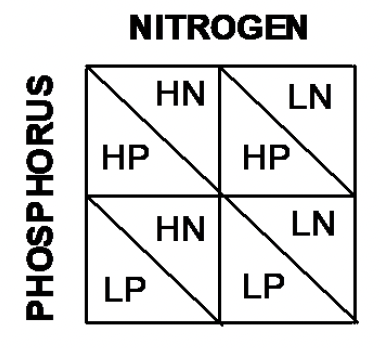
\includegraphics[width=0.4\linewidth]{figures/nitrogen_phosphorus} \caption{Blocked design}\label{fig:unnamed-chunk-47}
\end{figure}

Out of these treatments, 1. and 2. are termed Main Effects: these are the basic factor levels that we have varied. 3. is termed an Interaction term.

We may find that increasing the level of either N or P on their own increases yields. However, these effects may not be independent. When combined, high levels of both N \& P may increase yields by more than the sum of their individual effects (synergistic) or by less than the sum of their individual effects (antagonistic). Interaction effects are tested in exactly the same way as main effects, using an F-ratio. The ANOVA table is slightly modified:

\begin{longtable}[]{@{}cccccc@{}}
\toprule\noalign{}
Source & DF & Sum of Squares & Mean Square & F-Ratio & Probability \\
\midrule\noalign{}
\endhead
\bottomrule\noalign{}
\endlastfoot
Nitrogen & 1 & 376.04 & 376.04 & 108.74 & 0.000 \\
Phosphorus & 1 & 3.37 & 3.37 & 0.97 & 0.335 \\
Nitrogen * Phosphorus & 1 & 84.37 & 84.37 & 24.39 & 0.000 \\
Error & 20 & 69.19 & 3.45 & & \\
\end{longtable}

In this example there is a significant effect of nitrogen on yields, but not phosphorus. In addition, the significant interaction term indicates that the response of yields to nitrogen varies depending on the level of phosphorus. ANOVA can tell us when there are significant differences between the means of treatments, but it cannot identify which treatment differs from which other treatments. Post hoc tests are used to find where differences lie. Tukey's Honest Significant Difference is a widely used post-hoc test. Post-hoc tests are briefly explored in the practical. We will go on to look at how to test for relationships among different variables, as opposed to differences between them.

\hypertarget{practical-3---introduction-to-analysis-of-variance}{%
\section{Practical 3 - Introduction to Analysis of Variance}\label{practical-3---introduction-to-analysis-of-variance}}

\hypertarget{aims}{%
\subsection{Aims}\label{aims}}

The aim of this week's practical is to introduce the analysis of experimental data using one- and two- way analyses of variance (ANOVA). These analyses are used for testing for differences between treatments in fully randomised experiments. Note that other forms of experimental design, such as the randomised block and the Latin square require modified forms of ANOVA, although the basic ideas are the same.

\hypertarget{the-data-1}{%
\subsection{The Data}\label{the-data-1}}

We will be continuing with the rather agricultural theme for todays practical, the data are from one of the previous module leaders (Rob Freckleton) and are very appropriate for demonstrating key points around ANOVA. As an historical aside, this is also rather appropriate, as ANOVA and many other statistical analyses were designed by R. A. Fisher whilst working on long-term crop yield studies at Rothamsted.

Today we are going to look at data from two experiments:

\begin{itemize}
\tightlist
\item
  \textbf{Experiment 1.} Comparison of the yields of four different carrot varieties. In this experiment, six plots of each of the four varieties were grown, with the plots allocated to varieties in a completely random manner.
\item
  \textbf{Experiment 2.} Effects of light and sex on feeding behaviour in chickens. This experiment aimed to determine the effect of light colour and sex on the rate at which chickens feed. Feeding rates were measured as the number of pecks made in a 15 minute period. There were 24 cages in total, half of which were illuminated with white light, and half with red light. Half of the 12 white-light cages were allocated a male chicken, and half a female chicken, and the same for the 12 red-light cages. The treatments were allocated to cages in a completely randomised manner.
\end{itemize}

\hypertarget{task-1---setting-up-your-workspace-1}{%
\subsection{Task 1 - Setting up your workspace}\label{task-1---setting-up-your-workspace-1}}

Log into posit Cloud and return to your instance in the class work space. Set up a new script in posit Cloud. Once again you will probably want to tidy your environment using the following (\textbf{make sure you have last weeks script saved in your \texttt{scripts} folder first});

\begin{Shaded}
\begin{Highlighting}[]
\CommentTok{\# Clean up your environment}
\FunctionTok{rm}\NormalTok{(}\AttributeTok{list =} \FunctionTok{ls}\NormalTok{())}
\end{Highlighting}
\end{Shaded}

You will need to ensure that the packages \texttt{tidyverse} and \texttt{car} are installed and loaded to complete todays workshop, check Chapter \ref{workspace-setup} and Chapter \ref{script-setup} if you are unsure how to do this.

\hypertarget{c5t2}{%
\subsection{Task 2 - Checking the data}\label{c5t2}}

To start with we will just be focusing on the \texttt{carrot\_yields.csv} data set, you can find this in the \texttt{data} folder of the workspace. Load it into your workspace, naming the object \texttt{carrot\_yields} and perform your routine checks to make sure its all there and that R has correctly interpreted the variables. You can use some of the functions we explored in Chapter \ref{checking-the-data} if you need some help with this.

The data should consist on two columns, one column containing the dependent variable (carrot yields) and a second column containing the factor levels (varieties).

\hypertarget{c5t3}{%
\subsection{Task 3 - Making some basic plots}\label{c5t3}}

Now we can start to explore the data. Here we have four different varieties of carrot, we could use the \texttt{filter()} function to look at the distribution of each category seperatly but because we have four categoreies, this isnt terribly efficient. Instead the below code uses the \texttt{facet\_wrap()} function, this splits your data plots according to a given variable (in this case Variety). Have a go at running the below code;

\begin{Shaded}
\begin{Highlighting}[]
\NormalTok{carrot\_yields }\SpecialCharTok{\%\textgreater{}\%} \CommentTok{\# pipe your data set into ggplot}
  \FunctionTok{ggplot}\NormalTok{(., }\FunctionTok{aes}\NormalTok{(}\AttributeTok{x =}\NormalTok{ Yields)) }\SpecialCharTok{+} \CommentTok{\# Tell ggplot which variable is mapped onto the x axis}
  \FunctionTok{geom\_histogram}\NormalTok{(}\AttributeTok{bins =} \DecValTok{10}\NormalTok{) }\SpecialCharTok{+} \CommentTok{\# Plot a histogram with 10 bins}
  \FunctionTok{facet\_wrap}\NormalTok{(}\FunctionTok{vars}\NormalTok{(Variety)) }\CommentTok{\# Facet wrap the plot so that each variety is in its own panel}
\end{Highlighting}
\end{Shaded}

\begin{quote}
\begin{itemize}
\tightlist
\item
  Now try manipulating the code bin number and then compare your faceted histograms to a single histogram that includes all the data.
\end{itemize}
\end{quote}

When you don't have many observations per category it can also be helpful to visualise the data a little differently. If we plot the data as point data for each variety we can sometimes get a better idea of the spread of the data. Try using the following;

\begin{Shaded}
\begin{Highlighting}[]
\NormalTok{carrot\_yields }\SpecialCharTok{\%\textgreater{}\%} \CommentTok{\# pipe your data set into ggplot}
  \FunctionTok{ggplot}\NormalTok{(., }\FunctionTok{aes}\NormalTok{(}\AttributeTok{x =}\NormalTok{ Variety, }\AttributeTok{y =}\NormalTok{ Yields)) }\SpecialCharTok{+} \CommentTok{\# Tell ggplot which variable is mapped onto the each axis}
  \FunctionTok{geom\_point}\NormalTok{() }\CommentTok{\# Plot a scatter plot}
\end{Highlighting}
\end{Shaded}

\begin{quote}
\begin{itemize}
\tightlist
\item
  Visually inspect the data to assess their distributions, whether they are (approximately) normal and whether there appear to be differences between the means and variances of the varieties.
\end{itemize}
\end{quote}

\hypertarget{c5t4}{%
\subsection{Task 4 - Produce some descriptive statistics}\label{c5t4}}

Try using the \texttt{group\_by()} and \texttt{summarise()} functions to find the means and standard errors of the means for each of the yields of the four varieties.

\begin{quote}
\begin{itemize}
\tightlist
\item
  Do the treatment yields appear to differ and, if so, how do they differ?
\end{itemize}
\end{quote}

\hypertarget{task-5---experiment-1---one-way-anova}{%
\subsection{Task 5 - Experiment 1 - One-way ANOVA}\label{task-5---experiment-1---one-way-anova}}

Now that we have explored the data, we can start to play with some ANOVAs. The null hypothesis for the one-way ANOVA is that all groups are drawn from populations with the same mean. Therefore, if the probability of the null hypothesis being true is small, then there is evidence that the samples are taken from populations with different means.

\begin{quote}
\begin{itemize}
\tightlist
\item
  Before running the ANOVA, write down what you understand by the terms: Sums of Squares, Mean square and F-ratio.
\end{itemize}
\end{quote}

Remember that the analysis of variance (ANOVA) works by asking whether the variance between the experimental groups is as large, or larger, than the variance within the experimental groups. The F- ratio then compares these two quantities, by dividing the variance between groups by the variance within groups. The null hypothesis is that these are the same, i.e.~F = 1. The assumptions of ANOVA are that the data for all treatments are normally distributed and that the variances of all treatments are equal.

First check whether the assumption of equal variances among treatments is met, by checking the output from a Levenes test. Run this test and check the result (look back at Chapter \ref{levene-test} if you need help doing this).

\begin{quote}
\begin{itemize}
\tightlist
\item
  The null hypothesis for this test is that the variances of all the groups are the same. Does the probability indicate that this null hypothesis is likely to be true?
\item
  Are the assumptions of ANOVA met?
\end{itemize}
\end{quote}

Now we can run our ANOVA

\begin{Shaded}
\begin{Highlighting}[]
\NormalTok{lsmodel01 }\OtherTok{\textless{}{-}} \FunctionTok{aov}\NormalTok{(Yields }\SpecialCharTok{\textasciitilde{}}\NormalTok{ Variety, }\AttributeTok{data =}\NormalTok{ carrot\_yields)}
\CommentTok{\# Here we are creating an object to store our model in }
\CommentTok{\# the aov() function will perform our ANOVA and we are identifying our predictor and response variables on by placement on either side of the tilde }
\CommentTok{\# As in earlier chapters your dependent (response) variable needs to be before the tilde and the independent (predictor) variable needs to be after the tilde.}
\FunctionTok{summary}\NormalTok{(lsmodel01)}
\CommentTok{\# Summarises the results of your model stored in lsmodel01}
\end{Highlighting}
\end{Shaded}

The results should looks something like this;

\begin{verbatim}
> summary(lsmodel01)
            Df Sum Sq Mean Sq F value   Pr(>F)    
Variety      3 1097.7   365.9    18.9 1.65e-05 ***
Residuals   16  309.7    19.4                     
---
Signif. codes:  0 ‘***’ 0.001 ‘**’ 0.01 ‘*’ 0.05 ‘.’ 0.1 ‘ ’ 1
\end{verbatim}

\begin{quote}
\begin{itemize}
\tightlist
\item
  Can you see how this compares to the ANOVA tables shown above?
\item
  Can you explain how the value of the F-ratio in this table is calculated?
\item
  What would an F-ratio close to 1 indicate?
\item
  What does the probability attached to the F-ratio indicate about the mean yields of the varieties?
\end{itemize}
\end{quote}

The analysis indicates that there are some differences between the varieties of the groups but we do not know where these differences lie. To find this out, we are going to use a post hoc test. These operate like a series of pair-wise comparisons of the treatments, and will identify where significant differences exist between the means of the different varieties. To do this we will perform a Tuckey test, this is the most commonly reported post-hot test for ANOVA. Try running the following;

\begin{Shaded}
\begin{Highlighting}[]
\FunctionTok{TukeyHSD}\NormalTok{(lsmodel01, }\AttributeTok{conf.level=}\NormalTok{.}\DecValTok{95}\NormalTok{) }
\CommentTok{\# Perform a d Tuckey test on our ANOVA, stored in lsmodel01 with confidence levels of 95\%.}
\end{Highlighting}
\end{Shaded}

The output table indicates which pairs of treatment means are significantly different from one another. The \texttt{diff} collumn gives the difference in means between the two varieties, the \texttt{lwr} and \texttt{upr} columns give the upper and lower bounds for the 95\% confidence interval for the difference and the \texttt{p\ adj} shows whether there is a significant difference between comparisons.

\begin{quote}
\begin{itemize}
\tightlist
\item
  Which varieties are significantly different from one another?
\item
  Write a short summary of the results.
\item
  How could you represent these results in a graph?
\end{itemize}
\end{quote}

When we want to look at differences, a box plot or bar chart is often a good option. We can use \texttt{ggplot()} to do this, try running the following;

\begin{Shaded}
\begin{Highlighting}[]
\FunctionTok{ggplot}\NormalTok{(}\AttributeTok{data =}\NormalTok{ carrot\_yields, }\FunctionTok{aes}\NormalTok{(}\AttributeTok{x =}\NormalTok{ Variety, }\AttributeTok{y =}\NormalTok{ Yields)) }\SpecialCharTok{+}
  \FunctionTok{geom\_boxplot}\NormalTok{()}
\end{Highlighting}
\end{Shaded}

\begin{quote}
\begin{itemize}
\tightlist
\item
  Does the plot you just produced match the conclusions you drew from performing an ANOVA and Tuckey test?
\end{itemize}
\end{quote}

\hypertarget{first-boxplot}{%
\subsection{Task 6 - Experiment 2 - Two-way ANOVA}\label{first-boxplot}}

The analysis of Experiment 2 requires a two-way ANOVA since there are two factors in the experiment: light colour and sex. Note that you can have more than two factors in a multi-way ANOVA (although the more you have, the harder it can be to interpret the results).

Run through \textbf{Task 2} (\ref{c5t2}) and load the \texttt{pecking\_rates.csv} file into your workspace, naming the object \texttt{chickens}. Run through some standard data checks, and explore the data using plots and descriptives statistics (as described in \textbf{Tasks 2-4}, \ref{c5t2}, \ref{c5t3}, \ref{c5t4}).

Now try making a box plot to visualise these differences with the following code;

\begin{Shaded}
\begin{Highlighting}[]
\FunctionTok{ggplot}\NormalTok{(}\AttributeTok{data =}\NormalTok{ chickens, }\FunctionTok{aes}\NormalTok{(}\AttributeTok{x =}\NormalTok{ light, }\AttributeTok{y =}\NormalTok{ pecking\_rates, }\AttributeTok{fill =}\NormalTok{ sex)) }\SpecialCharTok{+}
  \FunctionTok{geom\_boxplot}\NormalTok{()}
\end{Highlighting}
\end{Shaded}

\begin{quote}
\begin{itemize}
\tightlist
\item
  What do you notice about the above code? How have we manipulated the \texttt{ggplot()} function to visualise two factors? Add some comments to your script to reflect the changes to the code.
\item
  From this plot, do you think chicken peck rates vary between the sexes and light colours?
\end{itemize}
\end{quote}

Hopefully you made some histograms when you were exploring the data, but if we are going to think about applying an ANOVA to these data we also need to check the other major ANOVA assumption.

Try running the following to check the assumption of equal variance;

\begin{Shaded}
\begin{Highlighting}[]
\FunctionTok{leveneTest}\NormalTok{(pecking\_rates }\SpecialCharTok{\textasciitilde{}}\NormalTok{ light }\SpecialCharTok{*}\NormalTok{ sex, }\AttributeTok{data =}\NormalTok{ chickens)}
\end{Highlighting}
\end{Shaded}

\begin{quote}
\begin{itemize}
\tightlist
\item
  What do you notice about the above code? Add comments to your script where appropriate.
\item
  What does the output of the Homogeneity test tell you?
\end{itemize}
\end{quote}

So lets try running a 2-way ANOVA, we can do this in a very similar way to before, but we are adding an additional factor plus an interaction \texttt{light:sex}. Try running the following;

\begin{Shaded}
\begin{Highlighting}[]
\NormalTok{lsmodel02 }\OtherTok{\textless{}{-}} \FunctionTok{aov}\NormalTok{(}\AttributeTok{formula =}\NormalTok{ pecking\_rates }\SpecialCharTok{\textasciitilde{}}\NormalTok{ light }\SpecialCharTok{+}\NormalTok{ sex }\SpecialCharTok{+}\NormalTok{ light}\SpecialCharTok{:}\NormalTok{sex, }\AttributeTok{data =}\NormalTok{ chickens)}
\FunctionTok{summary}\NormalTok{(lsmodel02)}
\end{Highlighting}
\end{Shaded}

The output looks more complex than the previous ANOVA output with a row for each factor plus a row for the interaction between factors.

\begin{quote}
\begin{itemize}
\tightlist
\item
  Do either or both of the main effects significantly influence the pecking rate?
\item
  Is there evidence of a significant interaction between Colour and Sex?
\item
  What does this interaction tell you about chicken pecking rates?
\item
  What would a non-significant interaction indicate?
\item
  Write down a short summary of the analysis.
\end{itemize}
\end{quote}

\hypertarget{conclusion-2}{%
\section{Conclusion}\label{conclusion-2}}

This week we have looked at some different types of experimental design and explored how we can visualise differences in R and perform one and two-way ANOVAs.

\hypertarget{before-you-leave-4}{%
\section{Before you leave!}\label{before-you-leave-4}}

Make sure you save your script and download it if you would like to keep a local copy.

Please log out of posit Cloud!

\hypertarget{references-3}{%
\section{References}\label{references-3}}

Wickham, H., Averick, M., Bryan, J., Chang, W., D'Agostino McGowan, L., François, R., Grolemund, G., et al., 2019. ``Welcome to the tidyverse.'' Journal of Open Source Software 4 (43): 1686. \url{https://doi.org/10.21105/joss.01686}.

\hypertarget{workshop-4---testing-for-and-measuring-relationships}{%
\chapter{Workshop 4 - Testing for and Measuring Relationships}\label{workshop-4---testing-for-and-measuring-relationships}}

\hypertarget{introduction-3}{%
\section{Introduction}\label{introduction-3}}

In this week's practical we are going to test for relationships or associations between different variables. There are two basic methods for testing for associations:

\begin{enumerate}
\def\labelenumi{\arabic{enumi})}
\tightlist
\item
  Correlation analysis measures the strength of the relationship between two variables.
\item
  Regression analysis is used to estimate an equation that best describes the effect of one variable upon another.
\end{enumerate}

In regression analysis, we are interested in the effect of an independent variable on a dependent variable. In scatter plots, the independent variable is always plotted on the horizontal x-axis, whilst the dependent variable is always plotted on the vertical y-axis.

\hypertarget{direction-of-associations}{%
\subsection*{Direction of associations}\label{direction-of-associations}}
\addcontentsline{toc}{subsection}{Direction of associations}

Regressions or correlations can be positive (y-values increase as x- values increase), negative (y-values decrease as x-values increase) or there may be no relationship (no change in y-values as x-values increase). The commonest form of regression analysis is linear regression, which fits a straight line to the relationship. In linear regression analysis, there are three key steps:

\begin{enumerate}
\def\labelenumi{\arabic{enumi})}
\tightlist
\item
  Find the line that best describes the association between the two variables and assess whether the slope of this is significantly different from zero.
\item
  Determine the strength of the relationship (how well the data fit the line).
\item
  Determine the coefficients (slope and intercept) of the equation that describes the line.
\end{enumerate}

The linear equation relates the dependent variable (y) to the independent variable (x), through two parameters:

\begin{itemize}
\tightlist
\item
  m is the slope: this is the rate of change in the y-variable as the x- variable increases. The larger the value of the slope, the faster y increases as x increases.
\item
  c is the intercept: this is the value of y when x is equal to zero. The intercept therefore measures the position of the line on the y-axis.
\end{itemize}

The parameter m is of greatest biological interest to us in regression analysis, as it measures the extent of change in y that results from a unit change in x.

\textbf{The regression equation}
\[
y=mx+c
\]

\begin{figure}
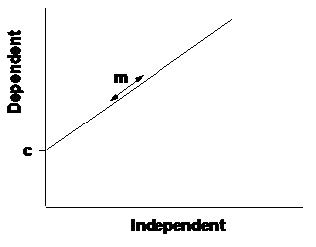
\includegraphics[width=0.4\linewidth]{figures/regression} \caption{Linear regression}\label{fig:unnamed-chunk-57}
\end{figure}

\hypertarget{fitting-the-regression}{%
\subsection*{Fitting the regression}\label{fitting-the-regression}}
\addcontentsline{toc}{subsection}{Fitting the regression}

Linear regression analysis basically works by finding the values of m and c that minimise the deviations of the observed data from the line (ie the distance of each point from the line). This is most commonly done using the least squares method, in which the squared deviations of the points from the line are minimised.

\begin{figure}
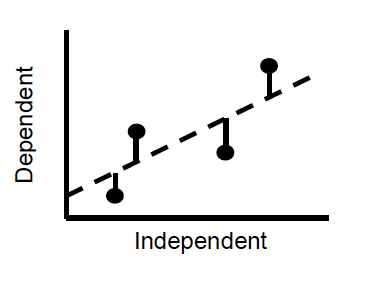
\includegraphics[width=0.4\linewidth]{figures/residuals} \caption{Fitting the regression}\label{fig:unnamed-chunk-58}
\end{figure}

The deviations of points from the fitted line are termed residuals, and the best fit line is the one with the lowest residual variation. The residual variation is thus the amount of variation in the data that is not explained by the line. The fit of the line is measured by r\(^2\), which is the proportion of the variance in y variable explained by x variable.

There are two ways to determine whether the relationship described by the fitted line is likely to have arisen by chance or not;

\begin{enumerate}
\def\labelenumi{\arabic{enumi})}
\item
  If there is no change in the y-values as x-values increase, the slope of the relationship is zero. We can therefore use a one-sample t-test to ask whether the slope of the relationship differs from a slope of zero. To do this, we need to compute a standard error for the slope, which is similar to the standard error of a mean. The SE of a slope measures our confidence in that slope, as it tells us where the true slope is likely to lie in relation to our estimate. Using n-2 DF we can calculate the 95\% confidence intervals for the slope from;
  \[
  m ± t*se 
  \]
  If these CIs do not overlap zero, then there is a greater than 95\% probability that the slope is different from zero, and we can then conclude that there is a significant relationship.
\item
  Alternatively, we can assess how different the slope is from zero by comparing the variance accounted for by the line with the total amount of variance in the y variable. If the line does not account for much of the variance in the data, then the overall variance will be much greater, and we cannot differentiate the slope from zero. This significance is assessed using an F-ratio in ANOVA.
\end{enumerate}

In fact these two tests are equivalent! The value of F is always the square of the value of t that we can estimate from the SE of the slope.

\hypertarget{assumptions}{%
\subsection*{Assumptions}\label{assumptions}}
\addcontentsline{toc}{subsection}{Assumptions}

There are 3 main assumptions, which are \textbf{different} from the assumptions of the tests for differences;

\begin{enumerate}
\def\labelenumi{\arabic{enumi})}
\tightlist
\item
  The deviations of points from the line (residuals) are evenly distributed along the line.
\item
  The variance of these residuals is constant across the range of values of x (homoscedasticity).
\item
  The measurement error in the x-axis is zero (or at least negligible in comparison to the error in the y-axis).
\end{enumerate}

\hypertarget{correlation}{%
\subsection*{Correlation}\label{correlation}}
\addcontentsline{toc}{subsection}{Correlation}

In some circumstances we are not attempting to measure the effect of one variable on another, we are just interested in the strength of association between two variables x and y, without inferring anything about the nature of cause and effect. The association between two variables is measured using the correlation coefficient, which measures the degree to which the joint variation in the data (the covariation) differs from the total variation in the data. This coefficient, denoted as r, is therefore a ratio that varies between -1 and 1, and measures the strength of the association between x and y;

\begin{itemize}
\tightlist
\item
  r = 1 indicates that two variables are perfectly positively correlated.
\item
  r = 0 indicates that two variables are entirely uncorrelated.
\item
  r = -1 indicates that two variables are perfectly negatively correlated.
\end{itemize}

It is important to be aware that the existence of a high correlation between two variables does not imply a cause-effect relationship. Quoting correlation coefficients without an understanding of the underlying patterns of association between variables is therefore dangerous. The covariation between two variables may simply be due to the effects of a third, unmeasured variable. Regression analysis should, therefore, only be applied when the cause-effect mechanism that is assumed in the regression equation is valid.

\hypertarget{practical-4---regression-correlation-introduction}{%
\section{Practical 4 - Regression \& Correlation Introduction}\label{practical-4---regression-correlation-introduction}}

This week we are going to look at statistical techniques involved in testing for associations between variables.

\hypertarget{the-data-2}{%
\subsection{The Data}\label{the-data-2}}

During the 1950s, radioactive waste leaked from a storage area into the Columbia River, Washington, USA. For nine counties downstream in Oregon, an index of exposure was calculated (based on distance from the leak site and average distance of the population from the river). The cancer mortality was also calculated for each county (deaths per 100,000 person-years, 1959-1964). Data were collected by Anderson and Sclove 1978

Because this data set is very small, we can enter this into R manually.

\hypertarget{manual-data-entry}{%
\subsection{Task 1 - Setting up your workspace}\label{manual-data-entry}}

Log into posit Cloud and return to your instance in the class work space. Set up a new script in posit Cloud. Once again you will probably want to tidy your environment using the following (\textbf{make sure you have last weeks script saved in your \texttt{scripts} folder first});

\begin{Shaded}
\begin{Highlighting}[]
\CommentTok{\# Clean up your environment}
\FunctionTok{rm}\NormalTok{(}\AttributeTok{list =} \FunctionTok{ls}\NormalTok{())}
\end{Highlighting}
\end{Shaded}

You will need to make sure the packages \texttt{tidyverse}, \texttt{performance} and \texttt{moderndive} are installed and loaded to complete todays workshop, check Chapter \ref{workspace-setup} and Chapter \ref{script-setup} if you are unsure how to do this.

As previously mentioned, the data set for this part of practical is relatively small, so we can enter it into R manually (this also gives you a chance to learn a little more code).

First of all we need to create a new object for each variable, and store our data accordingly. Try running the following;

\begin{Shaded}
\begin{Highlighting}[]
\NormalTok{exposure }\OtherTok{\textless{}{-}} \FunctionTok{c}\NormalTok{(}\FloatTok{8.3}\NormalTok{, }\FloatTok{6.4}\NormalTok{, }\FloatTok{3.4}\NormalTok{, }\FloatTok{3.8}\NormalTok{, }\FloatTok{2.6}\NormalTok{, }\FloatTok{11.6}\NormalTok{, }\FloatTok{1.2}\NormalTok{, }\FloatTok{2.5}\NormalTok{, }\FloatTok{1.6}\NormalTok{)}
\NormalTok{cancer }\OtherTok{\textless{}{-}} \FunctionTok{c}\NormalTok{(}\DecValTok{210}\NormalTok{, }\DecValTok{180}\NormalTok{, }\DecValTok{130}\NormalTok{, }\DecValTok{170}\NormalTok{, }\DecValTok{130}\NormalTok{, }\DecValTok{210}\NormalTok{, }\DecValTok{120}\NormalTok{, }\DecValTok{150}\NormalTok{, }\DecValTok{140}\NormalTok{)}
\end{Highlighting}
\end{Shaded}

Now we need to combine our individual variables into a single data frame, to do this we can use the function \texttt{tibble()}. Try running the following;

\begin{Shaded}
\begin{Highlighting}[]
\NormalTok{exposure\_cancer }\OtherTok{\textless{}{-}} \FunctionTok{tibble}\NormalTok{(exposure, cancer)}
\end{Highlighting}
\end{Shaded}

\begin{quote}
\begin{itemize}
\tightlist
\item
  Use some of the functions from Chapter \ref{checking-the-data} to exlore this data set.
\item
  Are you happy you understand how we generated the new dataframe?
\end{itemize}
\end{quote}

\hypertarget{c6t2}{%
\subsection{Task 2 - Making some basic plots}\label{c6t2}}

Lets start by taking a look at how your data are spread. We can do this by making a scatter plot. Last week we used \texttt{ggplot()} to make some boxplots and histograms, we can also use this function to make scatter plots. Try running the following;

\begin{Shaded}
\begin{Highlighting}[]
\CommentTok{\# Create a scatter plot to look at the relationship between radiation }
\FunctionTok{ggplot}\NormalTok{(}\AttributeTok{data=}\NormalTok{ exposure\_cancer, }\FunctionTok{aes}\NormalTok{(}\AttributeTok{x =}\NormalTok{ exposure, }\AttributeTok{y =}\NormalTok{ cancer)) }\SpecialCharTok{+}
  \FunctionTok{geom\_point}\NormalTok{()}
\end{Highlighting}
\end{Shaded}

Hopefully R has produced a scatter plot in your plots panel exploring the relationship between radiation exposure and cancer mortality.

\begin{quote}
\begin{itemize}
\tightlist
\item
  Does there appear to be any relationship between the cancer rate and radiation exposure?
\item
  What is the direction of the relationship?
\end{itemize}
\end{quote}

\hypertarget{c6t3}{%
\subsection{Task 3 - Regression analysis}\label{c6t3}}

On the basis of medical evidence, we have strong reasons to suspect that elevated radiation can cause increased cancer mortality. As this hypothesis specifies a cause-effect relationship, we can use a regression analysis to assess the extent to which this radioactive leak can explain the observed cancer mortality rates.

We can modify the scatter plot you made in Task 2 to fit a regression line or line of best fit to your plot. Try adding the following line to your scatter plot code (dont forget to add a \texttt{+} to pipe to your new line of code);

\begin{Shaded}
\begin{Highlighting}[]
 \FunctionTok{geom\_smooth}\NormalTok{(}\AttributeTok{method=}\StringTok{\textquotesingle{}lm\textquotesingle{}}\NormalTok{)}
\CommentTok{\# here we are instructing R to fit a line using the method \textasciigrave{}lm\textasciigrave{} which is an abbreviation of linear model}
\end{Highlighting}
\end{Shaded}

There are, of course, some assumptions about the data that must be checked before relying on the outputs from a regression analysis. The two key assumptions of linear regression are;

\begin{enumerate}
\def\labelenumi{\arabic{enumi})}
\tightlist
\item
  The deviations of points from the line (residuals) must be evenly distributed along the line.
\item
  The variance of these residuals must be constant across the range of values of x (homoscedasticity).
\end{enumerate}

You can often assess these assumptions with visual inspection of the graphs, and it can also help to plot the residuals (difference between the actual value of y and the value predicted from the equation) against the predicted values (values of y predicted from the equation for each value of x). Positive residuals indicate actual values that are greater than predicted values (i.e.~points that lie above the line), and negative residuals are less than the predicted values (i.e.~points lying below the line). If the regression assumptions are met, then a plot of residuals against predicted values should give a random scatter of points with no systematic pattern or bias. A positive or negative trend in this plot would indicate heteroscedasticity, a wedge-shape would indicate a greater spread of data at one end of the line and a U-shape would indicate a non-linear relationship.

First of all, lets build our model, try running the following;

\begin{Shaded}
\begin{Highlighting}[]
\NormalTok{model01 }\OtherTok{\textless{}{-}} \FunctionTok{lm}\NormalTok{(cancer }\SpecialCharTok{\textasciitilde{}}\NormalTok{ exposure, }\AttributeTok{data =}\NormalTok{ exposure\_cancer)}
\CommentTok{\# Here we are creating a new object called model01}
\CommentTok{\# In this object we are placing a linear model as described by the lm() function}
\CommentTok{\# We are then specifying that we want to analyse cancer (our response variable) as a function of exposure (our predictor variable) using tilde (\textasciitilde{}). We then just tell R which data frame we are using with the data = exposure\_cancer argument. }
\FunctionTok{summary}\NormalTok{(model01)}
\CommentTok{\# Summary() will just print out a summary of our model for us to interpret.}
\end{Highlighting}
\end{Shaded}

Don't worry too much about interpreting the summary table yet, first lets check some of our assumptions. We can plot out our residuals against our predicted values to check their distribution and homoscedasticity using the following piece of code, try running it now;

\begin{Shaded}
\begin{Highlighting}[]
\FunctionTok{ggplot}\NormalTok{(model01, }\FunctionTok{aes}\NormalTok{(}\AttributeTok{x =}\NormalTok{ .fitted, }\AttributeTok{y =}\NormalTok{ .resid)) }\SpecialCharTok{+}
  \FunctionTok{geom\_point}\NormalTok{()}
\end{Highlighting}
\end{Shaded}

You can also check to see where these data points have come from with the following;

\begin{Shaded}
\begin{Highlighting}[]
\FunctionTok{get\_regression\_points}\NormalTok{(model01)}
\CommentTok{\# export regression points in a table of outcome/response variable, all explanatory/predictor variables, the fitted/predicted value, and residuals.}
\end{Highlighting}
\end{Shaded}

By looking at these latest two outputs (your residuals vs predicted values plot and regression points table) try to answer the following;

\begin{quote}
\begin{itemize}
\tightlist
\item
  Do the residuals plot into a nice even band?
\item
  Is there any sign of a wedge-shaped distribution with an increase in variance at one end?
\item
  Is there any sign of a U-shape in the residual plot, indicating that non-linear regression might be needed?
\end{itemize}
\end{quote}

It is important to check thoroughly the assumptions of regression, as datapoints exerting a disproportionate influence can have dramatic impacts on the results. If all assumptions are met, you can now explore the regression output, rerun the \texttt{summary(model01)} line. You should get an output that looks like this;

\begin{verbatim}
> summary(model01)

Call:
lm(formula = cancer ~ exposure, data = exposure_cancer)

Residuals:
    Min      1Q  Median      3Q     Max 
-19.161 -11.934   3.741   8.969  17.226 

Coefficients:
            Estimate Std. Error t value Pr(>|t|)    
(Intercept)  118.449      8.365  14.161 2.08e-06 ***
exposure       9.033      1.480   6.103  0.00049 ***
---
Signif. codes:  0 ‘***’ 0.001 ‘**’ 0.01 ‘*’ 0.05 ‘.’ 0.1 ‘ ’ 1

Residual standard error: 14.58 on 7 degrees of freedom
Multiple R-squared:  0.8418,    Adjusted R-squared:  0.8192 
F-statistic: 37.24 on 1 and 7 DF,  p-value: 0.0004898
\end{verbatim}

There is a lot of information here so we will break each section down.

First of all we have a reminder of the formula we gave to the \texttt{lm()} function;

\begin{verbatim}
Call:
lm(formula = cancer ~ exposure, data = exposure_cancer)
\end{verbatim}

Then we have a summary of our residuals;

\begin{verbatim}
Residuals:
    Min      1Q  Median      3Q     Max 
-19.161 -11.934   3.741   8.969  17.226 
\end{verbatim}

We have already explored our residuals in some depth so I wont go into a huge amount of detail around this summary, you can read around it if it interests you.

Then we have our coefficients summary;

\begin{verbatim}
Coefficients:
            Estimate Std. Error t value Pr(>|t|)    
(Intercept)  118.449      8.365  14.161 2.08e-06 ***
exposure       9.033      1.480   6.103  0.00049 ***
---
Signif. codes:  0 ‘***’ 0.001 ‘**’ 0.01 ‘*’ 0.05 ‘.’ 0.1 ‘ ’ 1
\end{verbatim}

If we look at the \texttt{Estimate} column, the \texttt{(Intercept)} is the intercept in the traditional sense, this would be where the regression line meets the Y axis, when exposure is zero. So we can think of this as cancer mortality will be 118 deaths per 100, 000 when the radioactive exposure index is zero. Now if you look at the \texttt{exposure} \texttt{Estimate} this is 9.033, this represents the slope of the regression line. If we were to translate this into words we could think of this as for every unit increment in exposure, cancer mortality increases by c.9 deaths per 100, 000. We can test this theory mathematically.

Plug your intercept and slope values into the y = mx + c equation to estimate the mortality of a county with an exposure index of 6. You can do this by typing 9.003 * 6 + 118.449 into the console in R. Compare this output to the scatter plot for exposure and cancer mortality that we made earlier today.

Regarding the other values represented here, the \texttt{Std.\ Error} (Standard Error) measures the average amount that the coefficient estimates vary from the actual average value of our response variable. We can use these to calculate confidence intervals if required.

The \texttt{t\ values} represent our T statistic, this is simply the coefficient divided by the standard error. A large T statistic will have a small standard error proportionally to its coefficient, so the T statisitc is really saying that our coefficient is X standard errors away from zero and the larger the T statistic the more certain we can be that our coefficient is not zero. Finally we have our \texttt{Pr(\textgreater{}\textbar{}t\textbar{})} which represents our p value. This is calculated using our T statistics and a T distribution (as seen in lectures). The significance codes denoted by \texttt{*} help you interpret the size and significance threshold of the p value. These are essentially telling you how confident you can be that your coeffieient is not zero.

Next we have our Residual standard error and R\textsuperscript{2} values;

\begin{verbatim}
Residual standard error: 14.58 on 7 degrees of freedom
Multiple R-squared:  0.8418,    Adjusted R-squared:  0.8192 
\end{verbatim}

The \texttt{Residual\ standard\ error} helps describe how well our data fit the model. If we think of our residuals as the distances our observed data points are away from the regression line then our residual standard error is the average amount that the observed data points differ from the predicted data points, shown by the regression line, in units of Y.

We then have two R\textsuperscript{2} values. The \texttt{Multiple\ R-squared} value is mostly used if your model only has one predictor (as in this case). It tells us the percentage of variation within our responce (dependent) variable that is explained by our predictor (independent) variable. The \texttt{Adjusted\ R-squared} value is used when we have multiple predictor variables included in our model. It can be interpreted in the same was as the \texttt{Multiple\ R-squared} value but it shows the percentage of the variation in the response variable that is explained by all predictor variables. The differences in calculation are slightly nuanced, you dont need to worry about them here.

Finally we come to our F-statistic;

\begin{verbatim}
F-statistic: 37.24 on 1 and 7 DF,  p-value: 0.0004898
\end{verbatim}

When we run a linear regression our null hypothesis is that there is no relationship between our two variables, you could also think of this as the null hypothesis stating that the coefficients for your variables are zero. So the alternative hypothesis would be that your coefficients for at least one of your variables is not zero. The \texttt{F-statistic} and associated \texttt{p-value} tests this hypothesis. Once again the larger your F statistic the more likely your result is to be significant and we can then use the p-value to measure the probability of seeing an F-statistic of that size if the null hypothesis were true.

Now we know how the summary output for our model is broken down we can start to interpret our results, from the \texttt{summary()} output for \texttt{model01} try to answer the following;

\begin{quote}
\begin{itemize}
\tightlist
\item
  How strongly is the cancer rate related to the radiation exposure? (Remember - the R\textsuperscript{2} value tells you what proportion of the variation in y is explained by x, from 0 to 1).
\item
  Is this relationship statistically significant (look at the p-value, which indicates the overall significance of the regression)?
\item
  What is the slope of the regression line?
\item
  How much does the cancer rate increase for an increase in exposure of 1 unit?
\item
  For an increase in exposure of 20 units, how much would you expect the cancer rate to increase?
\item
  What is the intercept of the slope?
\item
  What does this intercept mean in real terms?
\item
  What is the standard error of the slope and what does this tell you?
\item
  Does the slope differ significantly from zero (look at the t-value of the slope, and the associated p value)? What does this tell you (bearing in mind that a slope of zero =no relationship).
\end{itemize}
\end{quote}

We can also calculate confidence intervals for the slope and the intercept. For example, we can be 95\% confident that the true values of our estimates lie somewhere between the upper and lower range of values given by the 95\% CIs. The confidence intervals are calculated from:

\textbf{Slope:}
\[
m ± t*se 
\]
\textbf{Intercept:}
\[
c ± t*se
\]
For 95\% CIs, there is a 5\% chance of the true value being outside these limits, thus there is a 2.5\% chance it is less than the lower limit and a 2.5\% chance it is greater than the upper limit. The appropriate t value for large degrees of freedom is 1.96, so if you want a crude estimate of the 95\% CIs, t = 2, ie ±2 standard errors from the estimate.

\begin{quote}
\begin{itemize}
\tightlist
\item
  Calculate the 95\% confidence intervals for the slope of the regression. What do these tell you? (Note: if you want to be precise, for 7 degrees of freedom, t = 2.365).
\item
  What cancer rate would you expect to find in a hypothetical county with an exposure index of 5? You can estimate this from the graph and calculate it from the regression equation.
\end{itemize}
\end{quote}

We often want to use fitted regressions to make predictions. These predictions can be made in two different ways;

\begin{enumerate}
\def\labelenumi{\arabic{enumi})}
\tightlist
\item
  \textbf{Predicted values:} predicting a mean value of y for a given value of x. If there were several counties with an exposure rate of 5, they would probably have slightly different cancer rates, due to natural variation. The cancer rate predicted from the regression equation is the mean rate for such counties. As this is a mean, it has a standard deviation, and the output also gives the 95\% confidence interval (CI). We can be 95\% sure that the mean lies between these upper and lower values.
\item
  \textbf{Prediction Intervals:} predicting a range (e.g.~95\%) of values of y for a given value of x. We call this the `prediction interval' (PI) to distinguish it from the `confidence interval' (CI) for the mean. Individual values are scattered around the mean, thus the PI for an individual county is wider than the CI for the mean of many counties.
\end{enumerate}

\begin{quote}
\begin{itemize}
\tightlist
\item
  What would you expect the cancer rate to be at an exposure index of 40?
\item
  Is this a valid prediction?
\end{itemize}
\end{quote}

\hypertarget{task-4---correlation-analysis}{%
\subsection*{Task 4 - correlation analysis}\label{task-4---correlation-analysis}}
\addcontentsline{toc}{subsection}{Task 4 - correlation analysis}

In cases where there is no biological reason to expect a cause-effect relationship, we can still assess the degree of association between two variables, by measuring the extent to which they co-vary (i.e.~as one variable changes, so does the other). The data listed below report the annual biomass of North Sea cod (in '000 tonnes), from 1980 to 2006.

In the \texttt{data} folder you should find a file called \texttt{cod\_biomass.csv}. Load this file into your workspace using the \texttt{read\_csv()} function. Use some of the commands from Chapter \ref{checking-the-data} to check the data and then use \texttt{ggplot()} to make a simple scatter plot. Try to answer the following questions;

\begin{quote}
\begin{itemize}
\tightlist
\item
  Does there appear to be a temporal trend in cod declines?
\item
  In which direction is the trend?
\end{itemize}
\end{quote}

Now we can calculate the Pearson (or product-moment) coefficient of correlation, using the command;

\begin{Shaded}
\begin{Highlighting}[]
\NormalTok{correlation01 }\OtherTok{\textless{}{-}} \FunctionTok{cor.test}\NormalTok{(cod\_biomass}\SpecialCharTok{$}\NormalTok{year, cod\_biomass}\SpecialCharTok{$}\NormalTok{cod\_biomass, }\AttributeTok{method =} \StringTok{"pearson"}\NormalTok{) }
\CommentTok{\# perform a correlation test on year and cod\_biomass in the cod\_biomass data set using Pearson\textquotesingle{}s correlation coefficient. }
\NormalTok{correlation01}
\CommentTok{\# print the information stored in correlation 01}
\end{Highlighting}
\end{Shaded}

\begin{quote}
\begin{itemize}
\tightlist
\item
  In the output the sample estimates is the correlation coefficient what does this value tell you?
\item
  What is the statistical significance of this association?
\item
  Could you have run a regression analysis on these data?
\end{itemize}
\end{quote}

\hypertarget{conclusion-3}{%
\section{Conclusion}\label{conclusion-3}}

This week we have looked at how we can analyse and interpret relationships, either through regression analysis or through correlation analysis.

\hypertarget{before-you-leave-5}{%
\section{Before you leave!}\label{before-you-leave-5}}

Make sure you save your script and download it if you would like to keep a local copy.

Please log out of posit Cloud!

\hypertarget{references-4}{%
\section{References}\label{references-4}}

Wickham, H., Averick, M., Bryan, J., Chang, W., D'Agostino McGowan, L., François, R., Grolemund, G., et al., 2019. ``Welcome to the tidyverse.'' Journal of Open Source Software 4 (43): 1686. \url{https://doi.org/10.21105/joss.01686}.

\hypertarget{workshop-5---issues-with-probability-and-parametric-analysis}{%
\chapter{Workshop 5 - Issues with Probability and Parametric Analysis}\label{workshop-5---issues-with-probability-and-parametric-analysis}}

\hypertarget{introduction-4}{%
\section{Introduction}\label{introduction-4}}

Statistical analyses allow us to estimate the probability that a given effect will occur by chance alone. As a matter of convention, if the probability of a given effect occurring is less than 1 in 20 (i.e.~p\textless0.05), then this effect is considered to be so unlikely to arise by chance that we can reject the null hypothesis of no difference or relationship.

There are two problems with using probability levels to determine whether an effect we see in our data is likely to be of significance;

\begin{enumerate}
\def\labelenumi{\arabic{enumi})}
\tightlist
\item
  Type I error occurs if we reject a null hypothesis when it is actually true (e.g.~our t-test indicates a statistically significant difference, but in fact the populations do not differ).
\item
  Type II error occurs if we accept a null hypothesis when it is in fact false (e.g.~our t-test does not indicate a statistically significant difference, when in fact the populations do differ).
\end{enumerate}

Both of these problems arise because we cannot state for certain whether two populations differ or whether two variables are related: we can only use the information at hand to state the probability. For example, if we conduct 100 tests of the same null hypothesis we would expect 5 to be statistically significant, even if the null hypothesis were true. When conducting a large number of tests of the same null hypothesis, we could partially overcome this problem by lowering our critical p-value. Alternatively, a technique called a sequential Bonferroni correction can be used to correct for a large number of tests of the same hypothesis. Often, however, the most sensible solution is to place more confidence in strongly (e.g.~p\textless0.001) than weakly (e.g.~p\textless0.05) significant results.

Ultimately, when we repeatedly test the same hypothesis, we cannot be completely certain that every effect we deem to be significant / non-significant is indeed so; we have to rely on an understanding of the system, and broad-scale patterns in our data, as much as rely on individual p values.

\hypertarget{non-normal-data-homogeneity-of-variance}{%
\subsection*{Non-normal data \& homogeneity of variance}\label{non-normal-data-homogeneity-of-variance}}
\addcontentsline{toc}{subsection}{Non-normal data \& homogeneity of variance}

The t and F distributions use information about the variance in estimates of population parameters, but they can only do this if a set of specific assumptions are met. All of the tests we have discussed so far rely on either data being normally distributed or residuals being evenly distributed. If this is not the case then all of the theory that predicts the likely behaviour of population parameters from our sampled estimates breaks down, and our tests are therefore invalid. This has been emphasised throughout, and we saw in an earlier practical how we could explore our data distribution using frequency histograms. Similarly, we saw that t-tests \& ANOVAs assume that the variances of all our groups are the same, whilst the regression analysis assumed that the variance in our dependent variable did not change with the value of our independent variable. We saw earlier how Levene's test could be used to test this assumption of homogeneity of variance.

If we find that either the assumption of normality or of homogeneity of variance is violated, then often it is possible to overcome the problem through transforming our data. In Figure 7.1, the upper graph shows data that are extremely skewed; the lower graph shows that when these data are log- transformed, they then appear very normal.

\begin{figure}
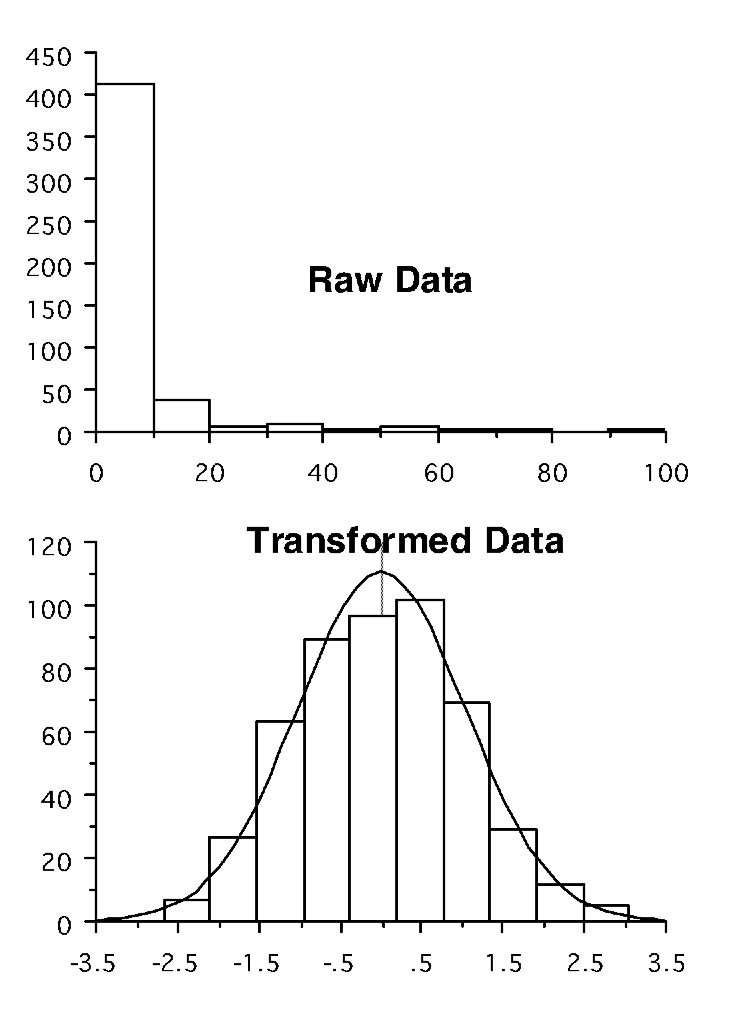
\includegraphics[width=0.4\linewidth]{figures/distributions} \caption{Impacts of log transformations - distribution}\label{fig:unnamed-chunk-68}
\end{figure}

Similarly, we can use a transformation of our data to meet the assumptions of regression analysis. In Figure 7.2, the upper scatter plot shows data that are inappropriate for linear regression, since the variance about the line increases with the value of the independent variable. The transformed data show a much more even distribution of residuals.

\begin{figure}
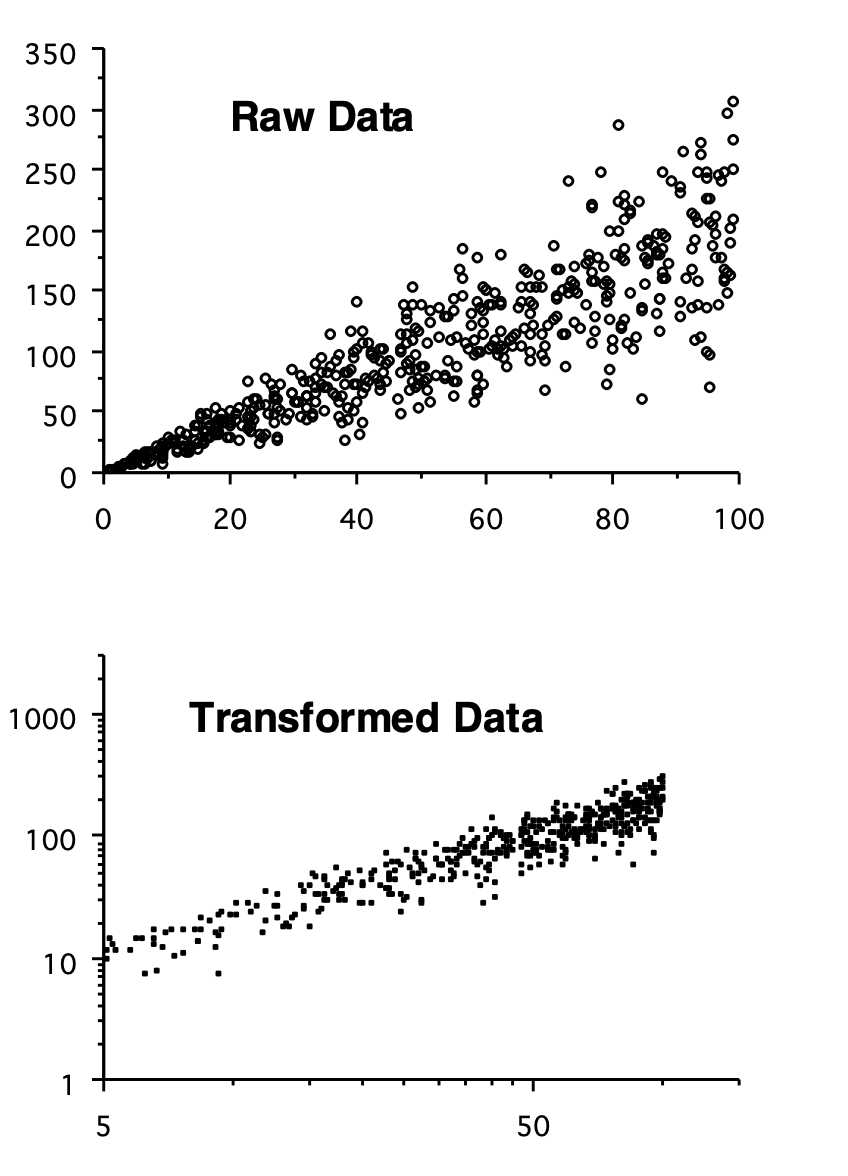
\includegraphics[width=0.4\linewidth]{figures/log_scatter} \caption{Impacts of log transformations - variance}\label{fig:unnamed-chunk-69}
\end{figure}

\hypertarget{transformations}{%
\subsection*{Transformations}\label{transformations}}
\addcontentsline{toc}{subsection}{Transformations}

A number of useful transformations exist;

\begin{enumerate}
\def\labelenumi{\arabic{enumi})}
\tightlist
\item
  \textbf{Logarithmic:} remember that the logarithm of a number x is the number to which 10 (or e) has to be raised in order to give x: e.g.~log10(100) = 2 since, 100 = 10\(^2\); log10(1000) = 3 since, 1000 = 10\(^3\), and so on.
\item
  \textbf{Logarithmic +1:} if we have some measurements of zero, or close to zero, then this may be a more effective transform that simply taking the logarithm. This is calculated as log(x+1).
\item
  \textbf{Square Root:} This operates in a similar fashion to the logarithmic transform and is especially used in regression analysis when the log-transform often goes a bit too far.
\item
  \textbf{Arcsine-square root:} This is used on proportional or percentage data, especially when the mean of the data is close to 0 or 1 (0 or 100\%). This is calculated as: sin\textsuperscript{-1}(\(\sqrt{x}\)). This helps to overcome the problem that such data are bounded, i.e.~not continuous.
\end{enumerate}

Transformation of data is a powerful and very important technique for overcoming the problem of non-normality and heterogeneity of variances. It is important to note, however that transforming data can affect our interpretation: e.g.~if we compare the mean of untransformed data, and the back-transformed mean of our transformed data, then these will not be the same. This should be borne in mind in interpreting results.

\hypertarget{non-parametric-methods}{%
\subsection*{Non-parametric methods}\label{non-parametric-methods}}
\addcontentsline{toc}{subsection}{Non-parametric methods}

In some cases it is not possible to transform data to a normal distribution. Data may also have been collected in ranks, or have measured an index of some variable we are interested in. To cope with these kinds of problems, a variety of statistical analyses have been developed that do not rely on assumptions about the distribution of data. They work somewhat differently, and in particular do not work by predicting the likely values of population parameters from statistics estimated from samples. In general, this is done in one of three ways;

\begin{enumerate}
\def\labelenumi{\arabic{enumi})}
\tightlist
\item
  \textbf{Median tests;} by analysing the median of the data, rather than the mean: you may remember that in the first practical we remarked that the median of our data is less sensitive to extreme values in our data and the skew of the distribution than the mean.
\item
  \textbf{Rank tests:} By ranking data, i.e.~sorting them into order and exploring the position of each observation. For example, in tests of differences, one group may rank higher than another and, in tests of association, the ranks of observations will be similar on both axes if an association exists.
\item
  \textbf{Patterns of deviation;} Or we can look at patterns of deviation, for example to say whether a prediction tends to systematically over- or under- predict on the basis of positive and negative differences, or whether higher than average scores (positive deviations) or one variable tend to be associated with higher than average scores in another.
\end{enumerate}

\hypertarget{non-parametric-tests-for-differences}{%
\subsection*{Non-parametric tests for differences}\label{non-parametric-tests-for-differences}}
\addcontentsline{toc}{subsection}{Non-parametric tests for differences}

The Mann-Whitney test is the non-parametric equivalent of the t- test. It is based on ranking data, and tests whether the location of one sample is different from that of another. This gives a statistic called U that, if greater than a critical value, indicates that there is a difference between the two groups.

The non-parametric equivalent to the one-way ANOVA (when we wish to test for differences between several rather than just two groups) is called a Kruskal-Wallis test. This yields a statistic H that, if greater than a critical level, indicates the existence of differences between our groups.

The most common design of two-way ANOVA is randomised block design, and the non-parametric equivalent for this is called Friedman's method for randomised blocks. For a regular two-way ANOVA, the Schreirer-Ray-Hare extension to the Kruskal-Wallis test may be employed (see Sokal \& Rohlf 1995; pp446-447).

\hypertarget{non-parametric-tests-for-association}{%
\subsection*{Non-parametric tests for association}\label{non-parametric-tests-for-association}}
\addcontentsline{toc}{subsection}{Non-parametric tests for association}

The most commonly employed non-parametric tests for association are Spearman's and Kendall's correlation coefficients, based again on ranking data. These both yield coefficients that are comparable to the correlation coefficient, and if greater in magnitude than a critical level indicate the existence of a significant correlation.

For regression analysis, a technique called Kendall's robust line-fit method, details of which may also be found in Sokal \& Rohlf (1995).

\hypertarget{pitfalls-of-non-parametric-tests}{%
\subsection*{Pitfalls of non-parametric tests}\label{pitfalls-of-non-parametric-tests}}
\addcontentsline{toc}{subsection}{Pitfalls of non-parametric tests}

Most of the tests mentioned above rely on ranking methods - they therefore have to be able to deal with the existence of ties in the data, i.e.~when two measurements have the same ranks. Often, when using these tests, you will see two outputs, one normal, and the other `corrected for ties'.

As you can probably guess from the names of these non- parametric tests, many mathematicians have sought fame and fortune through designing a `distribution-free analysis'. There are, therefore, many tests that do more or less the same thing, and which give basically the same results. Those mentioned above are generally the most commonly used. There are also methods for constructing models in which you can define the structure of the data (called generalised linear models), which we will explore in the next module.

\hypertarget{practical-5---transformations-non-parametric-tests---an-introduction}{%
\section{Practical 5 - Transformations \& Non-parametric Tests - An Introduction}\label{practical-5---transformations-non-parametric-tests---an-introduction}}

The techniques we have so far used to test for differences and associations are all parametric tests, which estimate population parameters from samples in order to test hypotheses. As we have seen, however, these tests make some assumptions about data that, if violated, would lead to results being invalid. In the previous classes we saw how we could check the assumptions of our analyses in order to determine whether the results will be valid. In this practical we are going to introduce some techniques that can be used if we believe that the assumptions of our parametric analysis have been violated. In the first section we will show how it is possible to transform data in order to overcome problems with the shape or variance of our data. In the second section we will introduce two simple non-parametric analyses, for use when our data either cannot be normalised, or when we have data (e.g.~counts, scores, ranks) that would be inappropriate for analysis with parametric techniques.

\hypertarget{task-1---setting-up-your-workspace-2}{%
\subsection{Task 1 - Setting up your workspace}\label{task-1---setting-up-your-workspace-2}}

Log into posit Cloud and return to your instance in the class work space. Set up a new script in posit Cloud. Once again you will probably want to tidy your environment using the following (\textbf{make sure you have last weeks script saved in your \texttt{scripts} folder first});

\begin{Shaded}
\begin{Highlighting}[]
\CommentTok{\# Clean up your environment}
\FunctionTok{rm}\NormalTok{(}\AttributeTok{list =} \FunctionTok{ls}\NormalTok{())}
\end{Highlighting}
\end{Shaded}

You will need to make sure that the package \texttt{tidyverse} is installed and loaded to complete todays workshop, check Chapter \ref{workspace-setup} and Chapter \ref{script-setup} if you are unsure how to do this.

The data for the first part of todays practical are the weights (g) of individual plants originating from seed taken from two sites. Each was grown singly in pots in a greenhouse, with the arrangement of pots being completely random.

The data set for this part of practical is relatively small, so as in the previous chapter, we can enter it into R manually.

First of all create two objects called \texttt{site1} and \texttt{site2} and fill them with the following data points (check Chapter \ref{manual-data-entry});

\begin{verbatim}
Site 1; 0.142, 0.084, 0.029, 0.175, 0.047, 0.012, 0.042, 0.200, 0.973, 0.158
Site 2; 1.304, 1.647, 0.269, 0.209, 0.131, 0.818, 4.571, 9.377, 0.204, 0.169
\end{verbatim}

Once you have your \texttt{site1} and \texttt{site2} objects you can then use the \texttt{tibble()} function to create a data frame called \texttt{seeds}.

Use \texttt{view()} to inspect your new data frame.

\begin{quote}
\begin{itemize}
\tightlist
\item
  What do you notice about the layout of these data?
\item
  Are these data in a long or a wide format?
\item
  What kind of format do we need them to be in?
\end{itemize}
\end{quote}

Hopefully you identified that the data in \texttt{seeds} are in a wide format and we need them in a long format. Tidyverse has a lot of very helpful functions for wrangling data into the format that we need it to be in. Here, we can use the \texttt{pivot\_longer()} function to manipulate our data. Try running the following, taking time to read each line of code and understand what each section does;

\begin{Shaded}
\begin{Highlighting}[]
\NormalTok{seeds2 }\OtherTok{\textless{}{-}}\NormalTok{ seeds }\SpecialCharTok{\%\textgreater{}\%}
  \FunctionTok{pivot\_longer}\NormalTok{(}\AttributeTok{cols =}\NormalTok{ site1}\SpecialCharTok{:}\NormalTok{site2,}
             \AttributeTok{names\_to =} \StringTok{"site"}\NormalTok{, }
             \AttributeTok{values\_to =} \StringTok{"weight"}\NormalTok{)}
\CommentTok{\# Here we are piping out initial seeds data set into the pivot\_longer() function}
\CommentTok{\# We are then telling the function which columns we with to be included within the seeds data frame}
\CommentTok{\# The names\_to argument is allowing us to name our categorical variable }
\CommentTok{\# The values\_to argument is allowing us to name our numeric variable}
\CommentTok{\# We are then saving the output from this function to the object seeds2}
\end{Highlighting}
\end{Shaded}

Now use the \texttt{view()} function on your new \texttt{seeds2} data frame, can you identify what the \texttt{pivot\_longer()} function has done?

\hypertarget{c7t2}{%
\subsection{Task 2 - Explore the data}\label{c7t2}}

Spend a little time exploring the data. Try using the \texttt{group\_by()} and \texttt{summarise()} functions to find the means, standard deviation and the standard error of the plant weights for each site (see Chapter \ref{descriptive-statistics} if you need help with this). Build some histograms to explore data distribution and maybe consider building a boxplot to explore differences between sites (see Chapter \ref{histogram} if you need help with this).

\begin{quote}
\begin{itemize}
\tightlist
\item
  Does there appear to be any difference between the two sites?
\item
  Does the distribution of data appear to be normal? (remember we have only a small number of observations so we would hardly expect a perfect bell-shaped pattern).
\end{itemize}
\end{quote}

Now try comparing the two sites with a levenes and a two sample t-test (check Chapter \ref{levene-test} if you're not sure how to do this).

\begin{quote}
\begin{itemize}
\tightlist
\item
  Does this test indicate that the two groups differ?
\item
  What does the Levene's test tell you about the variances of the two groups?
\item
  What are the assumptions of a t-test, and do you think that these data conform to them?
\end{itemize}
\end{quote}

\hypertarget{c7t3}{%
\subsection{Task 3 - Data transformations}\label{c7t3}}

Basically there are two problems with these data;

\begin{enumerate}
\def\labelenumi{\arabic{enumi})}
\tightlist
\item
  The data (particularly those from site 2) are highly skewed
\item
  The variances for the two groups are very different, which could mean that a parametric test may fail to detect a difference, if it exists (although if the difference between the two groups is very large, a parametric test may detect the difference despite the assumptions not being met).
\end{enumerate}

We can attempt to meet these assumptions by transforming the data. Since the data are spread over several orders of magnitude (e.g.~in site 1 we have values ranging from 0.012 to 0.142: the former measurement is ten times the size of the latter), a logarithmic transformation is likely to be appropriate.

Thankfully this is a very easy addition we can make in our \texttt{seeds2} dataframe. Try running the following piece of code;

\begin{Shaded}
\begin{Highlighting}[]
\NormalTok{seeds2 }\OtherTok{\textless{}{-}}\NormalTok{ seeds2 }\SpecialCharTok{\%\textgreater{}\%}
  \FunctionTok{mutate}\NormalTok{(}\AttributeTok{log10 =} \FunctionTok{log10}\NormalTok{(seeds2}\SpecialCharTok{$}\NormalTok{weight))}
\end{Highlighting}
\end{Shaded}

Use the \texttt{view()} command to take a look at your \texttt{seeds2} dataframe.

\begin{quote}
\begin{itemize}
\tightlist
\item
  The log10 expression means to take the logarithm to the base 10. With this in mind, do you understand what the mutate() function has done?
\item
  Add some appropriate comments to your script to describe the above code.
\end{itemize}
\end{quote}

Repeat the data explorations that you carried our in Chapter \ref{c7t2} on the new log10 column.

\begin{quote}
\begin{itemize}
\tightlist
\item
  Is there still a difference between the two sites? (Remember that the true population mean for each group will lie within approximatly 2 standard errors either side of the mean)
\item
  How does the distribution of data compare with what we saw before?
\end{itemize}
\end{quote}

Carry our a levenes test and two sample t-test on the two log transformed groups.

\begin{quote}
\begin{itemize}
\tightlist
\item
  Does this test indicate that the two groups differ?
\item
  What does the Levene's test tell you this time about the variances of the two groups?
\item
  How do these results compare with the analysis of the un-transformed data?
\end{itemize}
\end{quote}

The transformation of the data has basically achieved what we wanted: the variances of the two groups are now not statistically different, and the transformed data are considerably less skewed than the raw data. A t-test comparison of these data is more likely to yield robust results.

\hypertarget{task-4---non-parametric-analysis-of-the-differences}{%
\subsection{Task 4 - Non-parametric analysis of the differences}\label{task-4---non-parametric-analysis-of-the-differences}}

One of the most striking features of the original data is that most of the larger values are for the data for site 2, whilst most of the smallest values are for site 1. This is very clear if we sort the data into order, and give each pot a rank:

\begin{figure}
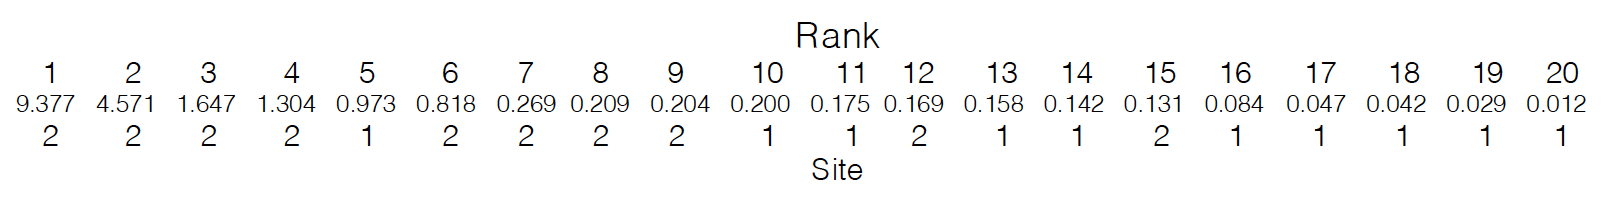
\includegraphics[width=0.9\linewidth]{figures/ranks} \caption{Rank Orders}\label{fig:unnamed-chunk-73}
\end{figure}

Work out the mean ranks of the pots taken from the two sites (you can either do this manually or see if you can write a piece of R code to do this).

\begin{quote}
\begin{itemize}
\tightlist
\item
  Do these mean ranks tell you whether one site tends to produce bigger plants than the other?
\end{itemize}
\end{quote}

In the top 10 positions, only 2 pots are from site 1, whilst in the last 10 positions, only 2 pots are from site 2. Clearly, irrespective of the spread or mean of these data, the plants from site 2 tend to be bigger than those from site 1. This is the basis for the first non-parametric test that we are going to look at, the Mann-Whitney test. This test simply compares the ranks of the data from our two groups, and determines whether one of the groups tends to occupy the top or bottom positions more frequently than we would expect by chance.

Copy over the following piece of code and run it from your script;

\begin{Shaded}
\begin{Highlighting}[]
\CommentTok{\# Mann Whitney U / Wilcoxan }
\FunctionTok{wilcox.test}\NormalTok{(weight }\SpecialCharTok{\textasciitilde{}}\NormalTok{ site, }\AttributeTok{data=}\NormalTok{seeds2) }
\end{Highlighting}
\end{Shaded}

Although this is called a Wilcoxon test, if you run the test on two independent samples (as we have here), R runs a Mann-Whitney U test (confusing I know). Here we have performed a Mann-Whitney U test. The W value is our test statistic and p-value is fairly self explanatory. The key statistic to look at is W (if you are familiar with MannWhitney U tests, this is equivelent to the traditional U value): this measures the difference between the ranks for the two groups; a large value indicates a large difference in ranks.

\begin{quote}
\begin{itemize}
\tightlist
\item
  The null hypothesis is that there is no difference between the groups: does the probability value indicate that this is likely to be the case?
\end{itemize}
\end{quote}

The non-parametric test works very differently to the t-test - in particular it ignores any information on the mean and variance in the data. Note that strictly speaking, it tells us whether the location of the data from two groups is different, not whether the means are different.

\hypertarget{task-5---non-parametric-test-for-associations}{%
\subsection{Task 5 - Non-parametric test for associations}\label{task-5---non-parametric-test-for-associations}}

Finally we are going to look at a non-parametric test that enables us to tell whether there is a significant association between two variables.

The data are taken from a study on aphids: \texttt{mother} records the total length of 15 aphid stem mothers, and \texttt{offspring} records the mean thorax length of their (numerous) parthenogenetic offspring, taken from visual estimates under a microscope.

\begin{verbatim}
mother; 8.70, 8.50, 9.40, 10.00, 6.30, 7.80, 11.90, 6.50, 6.60, 10.60, 10.20, 7.20, 8.60, 11.10, 11.60 
offspring; 5.95, 5.65, 6.00, 5.70, 4.70, 5.53, 6.40, 4.18, 6.15, 5.93, 5.70, 5.68, 6.13, 6.30, 6.03 
\end{verbatim}

Use the above data to create a new data frame called aphids, with two 2 columns titled; mother and offspring. Create a scatter plot to see whether there appears to be any association between these two variables.

\begin{quote}
\begin{itemize}
\tightlist
\item
  What would be the problem with using parametric correlation or regression analyses to look at this association?
\end{itemize}
\end{quote}

Basically there are two problems here;

\begin{enumerate}
\def\labelenumi{\arabic{enumi})}
\tightlist
\item
  There is error in both axes: the lengths of the mothers are estimated rather than accurately measured and the offspring lengths are averages.
\item
  The pattern of association is not linear: the significance test for a parametric correlation coefficient requires a linear association.
\end{enumerate}

There are two (very similar) non-parametric measures of correlation. These again rely on ranks: i.e.~they test whether high-ranking mothers produce high ranking offspring.

First of all try running the following to have R assign a rank to each of the variables;

\begin{Shaded}
\begin{Highlighting}[]
\NormalTok{aphids }\OtherTok{\textless{}{-}}\NormalTok{ aphids }\SpecialCharTok{\%\textgreater{}\%}
  \FunctionTok{mutate}\NormalTok{(}\AttributeTok{rank\_m =} \FunctionTok{rank}\NormalTok{(aphids}\SpecialCharTok{$}\NormalTok{mother)) }\SpecialCharTok{\%\textgreater{}\%}
  \FunctionTok{mutate}\NormalTok{(}\AttributeTok{rank\_o =} \FunctionTok{rank}\NormalTok{(aphids}\SpecialCharTok{$}\NormalTok{offspring))}
\end{Highlighting}
\end{Shaded}

\begin{quote}
\begin{itemize}
\tightlist
\item
  Do you understand what each line of code is doing here? Try to add comments to it in your script.
\end{itemize}
\end{quote}

If there is a correlation then we would expect the biggest mother to have the biggest offspring, and the smallest mother to have the smallest offspring. Create a scatter plot from your ranked variables.

\begin{quote}
\begin{itemize}
\tightlist
\item
  Does it appear that the rank of the offspring follows that of the mother?
\end{itemize}
\end{quote}

We can see if there is a correlation using the Spearmans Rank correlation coefficient. Try running the following;

\begin{Shaded}
\begin{Highlighting}[]
\FunctionTok{cor.test}\NormalTok{(aphids}\SpecialCharTok{$}\NormalTok{mother, aphids}\SpecialCharTok{$}\NormalTok{offspring, }\AttributeTok{method =} \StringTok{"spearman"}\NormalTok{)}
\end{Highlighting}
\end{Shaded}

You will get the following warning;

\begin{verbatim}
Warning message:
In cor.test.default(aphids$mother, aphids$offspring, method = "spearman") :
  Cannot compute exact p-value with ties
\end{verbatim}

This is because some of the ranks are tied in the offspring variable. We can edit our code so that we can still get an estimate of the correlation coefficient by editing our command to read as follows;

\begin{Shaded}
\begin{Highlighting}[]
\FunctionTok{cor.test}\NormalTok{(aphids}\SpecialCharTok{$}\NormalTok{mother, aphids}\SpecialCharTok{$}\NormalTok{offspring, }\AttributeTok{method =} \StringTok{"spearman"}\NormalTok{, }\AttributeTok{exact =} \ConstantTok{FALSE}\NormalTok{)}
\end{Highlighting}
\end{Shaded}

The coefficients that this analysis generates are structured in the same way as the normal (Pearson's) correlation coefficient: a magnitude of 1 indicates perfect positive correspondence; a value of 0 indicates no association.

\begin{quote}
\begin{itemize}
\tightlist
\item
  What does the coefficient tell you?
\item
  Is it statistically significant?
\end{itemize}
\end{quote}

\hypertarget{conclusion-4}{%
\section{Conclusion}\label{conclusion-4}}

Today we have explored how to deal with data that breaks the assumptions made by parametric tests. We have seen what the impact of log transformations and ranking data has on its structure and have played with a few non-parametric tests to test for differences and associations.

\hypertarget{before-you-leave-6}{%
\section{Before you leave!}\label{before-you-leave-6}}

Make sure you save your script and download it if you would like to keep a local copy.

Please log out of posit Cloud!

\hypertarget{references-5}{%
\section{References}\label{references-5}}

Wickham, H., Averick, M., Bryan, J., Chang, W., D'Agostino McGowan, L., François, R., Grolemund, G., et al., 2019. ``Welcome to the tidyverse.'' Journal of Open Source Software 4 (43): 1686. \url{https://doi.org/10.21105/joss.01686}.

\hypertarget{plot-beautification}{%
\chapter{Plot Beautification!!!}\label{plot-beautification}}

So far, in this workbook, we have used a number of different plots to explore our data. They have served their job well and given you a good overview of what the data look like. Which is absolutely fine, while you are tinkering and exploring with your data sets. However, that wont fly when it comes to sharing your analysis outputs; be that in a summative coursework piece, a presentation (verbal or poster) or a professional publication. Thankfully, \texttt{ggplot()} has some fantastic features for making plots look absolutely stunning, and we can quickly make a draft plot look absolutely fabulous very quickly.

This is a crash course in plot beautification using \texttt{ggplot()}. It is by no means an exhaustive list of all the aesthetic parameters you can edit, but it will give you a good grounding.

\hypertarget{deconstructing-ggplot}{%
\section{Deconstructing ggplot}\label{deconstructing-ggplot}}

Hopefully you have been saving the code from former workshops in a sensible place in our posit Cloud classroom. Back in Chapter \ref{first-boxplot} we made a boxplot comparing the pecking rates between male and female chickens. Initially, we will work with this same plot.

Log into posit Cloud and join the class workspace. Clean-up your enironment with the following command;

\begin{Shaded}
\begin{Highlighting}[]
\CommentTok{\# Clean up your environment}
\FunctionTok{rm}\NormalTok{(}\AttributeTok{list =} \FunctionTok{ls}\NormalTok{())}
\end{Highlighting}
\end{Shaded}

Now load your script from Practical 3, Chapter \ref{differences}, install and load the \texttt{tidyverse} package and create a \texttt{chickens} object containing the \texttt{pecking\_rates.csv}.

To get an idea of how ggplot works we are going to go back over some code you have already run. Try running the following, what happens?

\begin{Shaded}
\begin{Highlighting}[]
\CommentTok{\# Making a box plot and saving it in an object}
\CommentTok{\# Call the ggplot function and direct it to your data, define your x axis and y axis and colour your plots by sex}
\NormalTok{pecking\_rates\_box }\OtherTok{\textless{}{-}} \FunctionTok{ggplot}\NormalTok{(}\AttributeTok{data =}\NormalTok{ chickens,}\AttributeTok{aesdata =}\NormalTok{ chickens, }\FunctionTok{aes}\NormalTok{(}\AttributeTok{x =}\NormalTok{ light, }\AttributeTok{y =}\NormalTok{ pecking\_rates, }\AttributeTok{fill =}\NormalTok{ sex)) }
\FunctionTok{print}\NormalTok{(pecking\_rates\_box) }\CommentTok{\# Print the object your plot is stored in to view it}
\end{Highlighting}
\end{Shaded}

So you have given ggplot your data set and specified the axes. But you haven't told it how you would like the data to be visualised. So you should see something like this\ldots{}

\begin{figure}
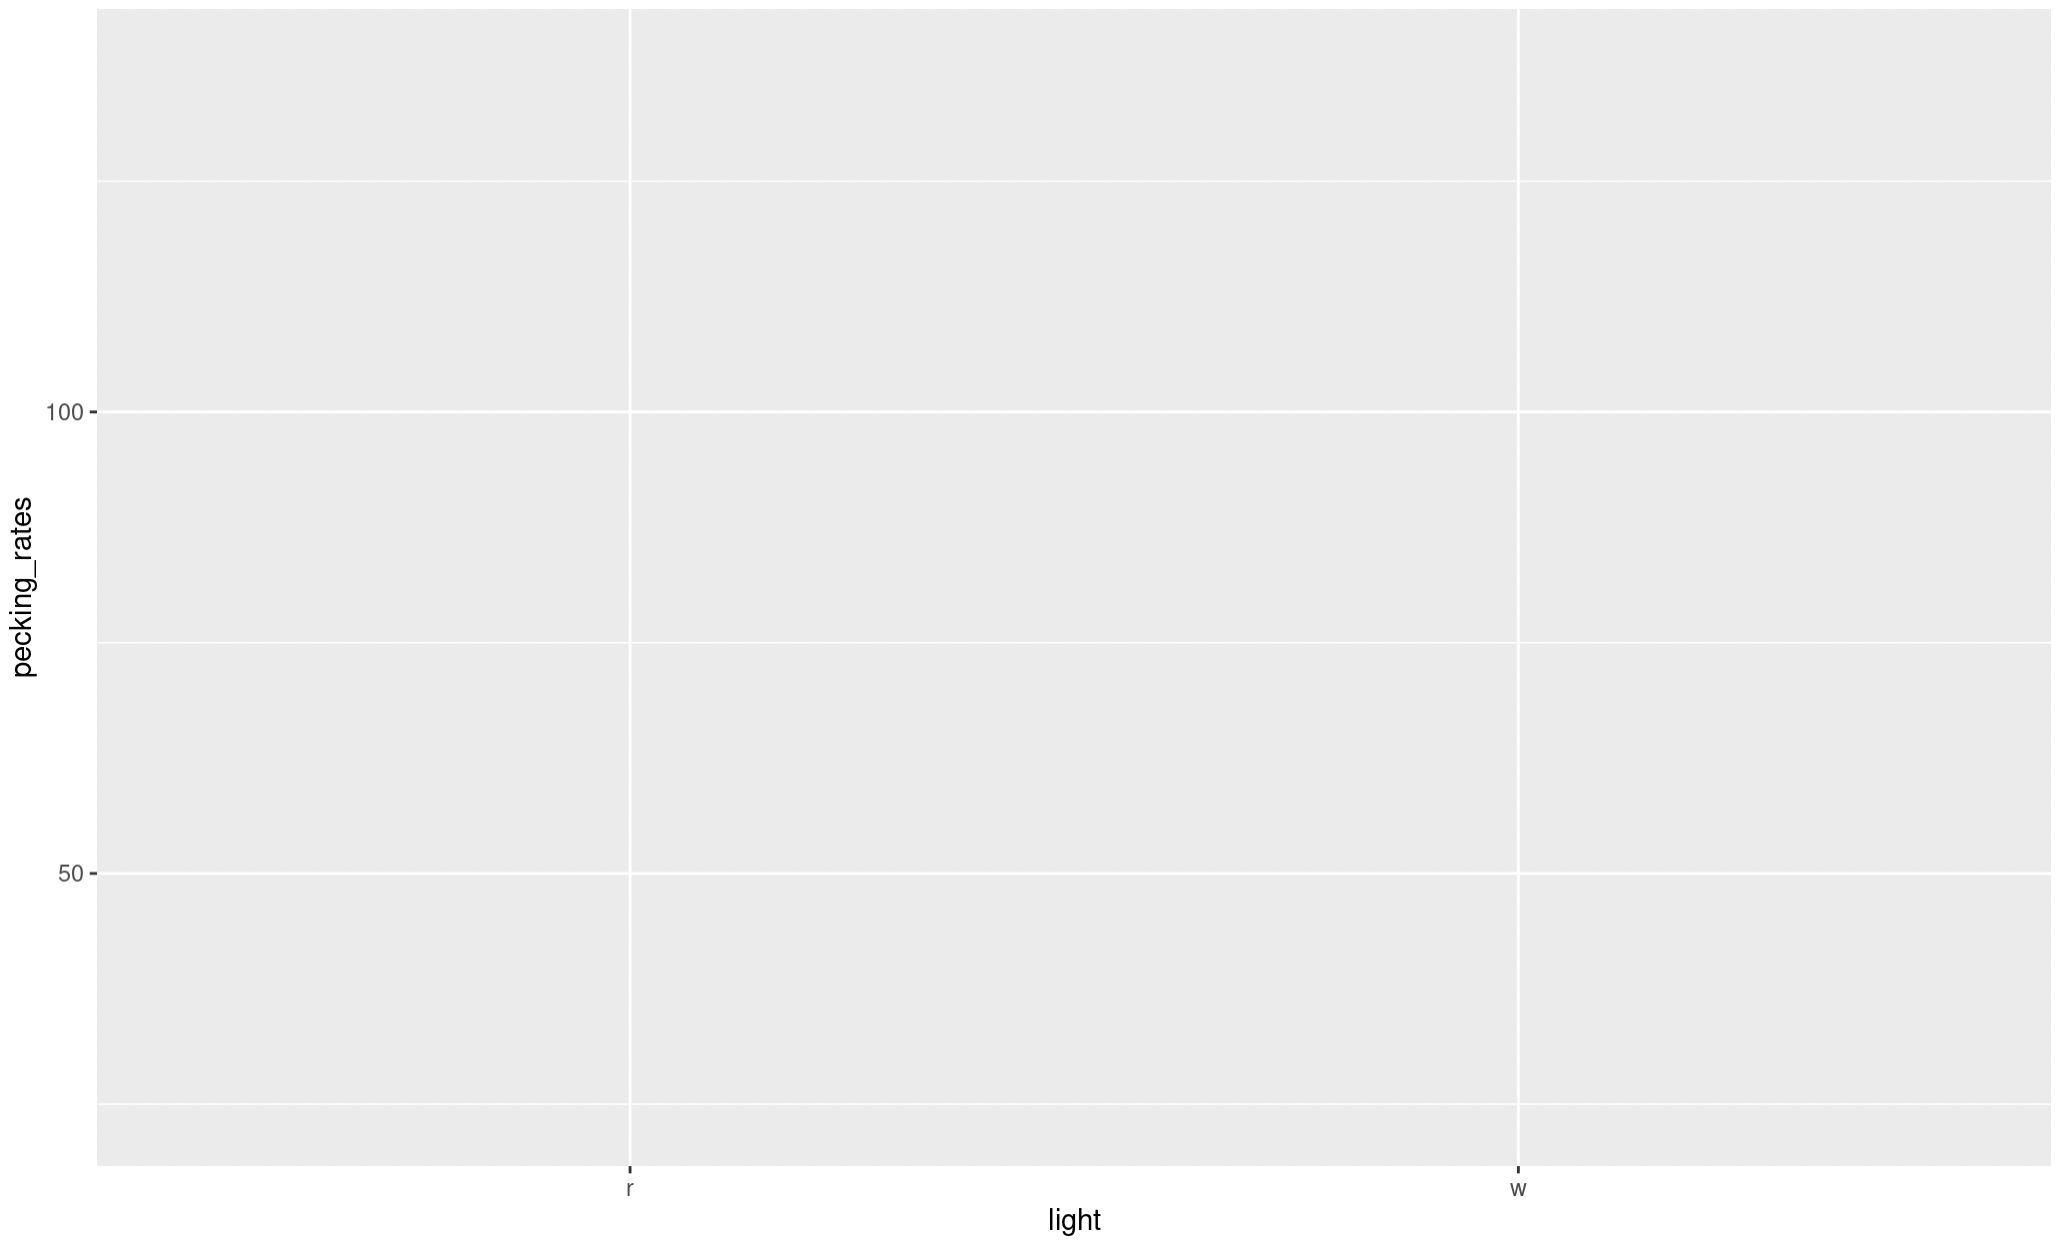
\includegraphics[width=0.9\linewidth]{figures/pecking_rates_1} \caption{The most basic output from ggplot}\label{fig:unnamed-chunk-80}
\end{figure}

Now modify the script so that it looks like this\ldots{}

\begin{Shaded}
\begin{Highlighting}[]
\CommentTok{\# Making a box plot and saving it in an object}
\CommentTok{\# Call the ggplot function and direct it to your data, define your x axis and y axis and colour your plots by sex}
\NormalTok{pecking\_rates\_box }\OtherTok{\textless{}{-}} \FunctionTok{ggplot}\NormalTok{(}\AttributeTok{data =}\NormalTok{ chickens,}\AttributeTok{aesdata =}\NormalTok{ chickens, }\FunctionTok{aes}\NormalTok{(}\AttributeTok{x =}\NormalTok{ light, }\AttributeTok{y =}\NormalTok{ pecking\_rates, }\AttributeTok{fill =}\NormalTok{ sex)) }\SpecialCharTok{+}
  \FunctionTok{geom\_boxplot}\NormalTok{() }\CommentTok{\# Tell ggplot that you want it to build a box plot}
\FunctionTok{print}\NormalTok{(pecking\_rates\_box) }\CommentTok{\# Print the object your plot is stored in to view it}
\end{Highlighting}
\end{Shaded}

Note the \texttt{+}, this is essentially another way of piping information from one function into the next. You could also have added \texttt{fill\ =\ sex} to an \texttt{aes()} function within the \texttt{geom\_boxplot()} function.

Your figure should look like this\ldots{}

\begin{figure}
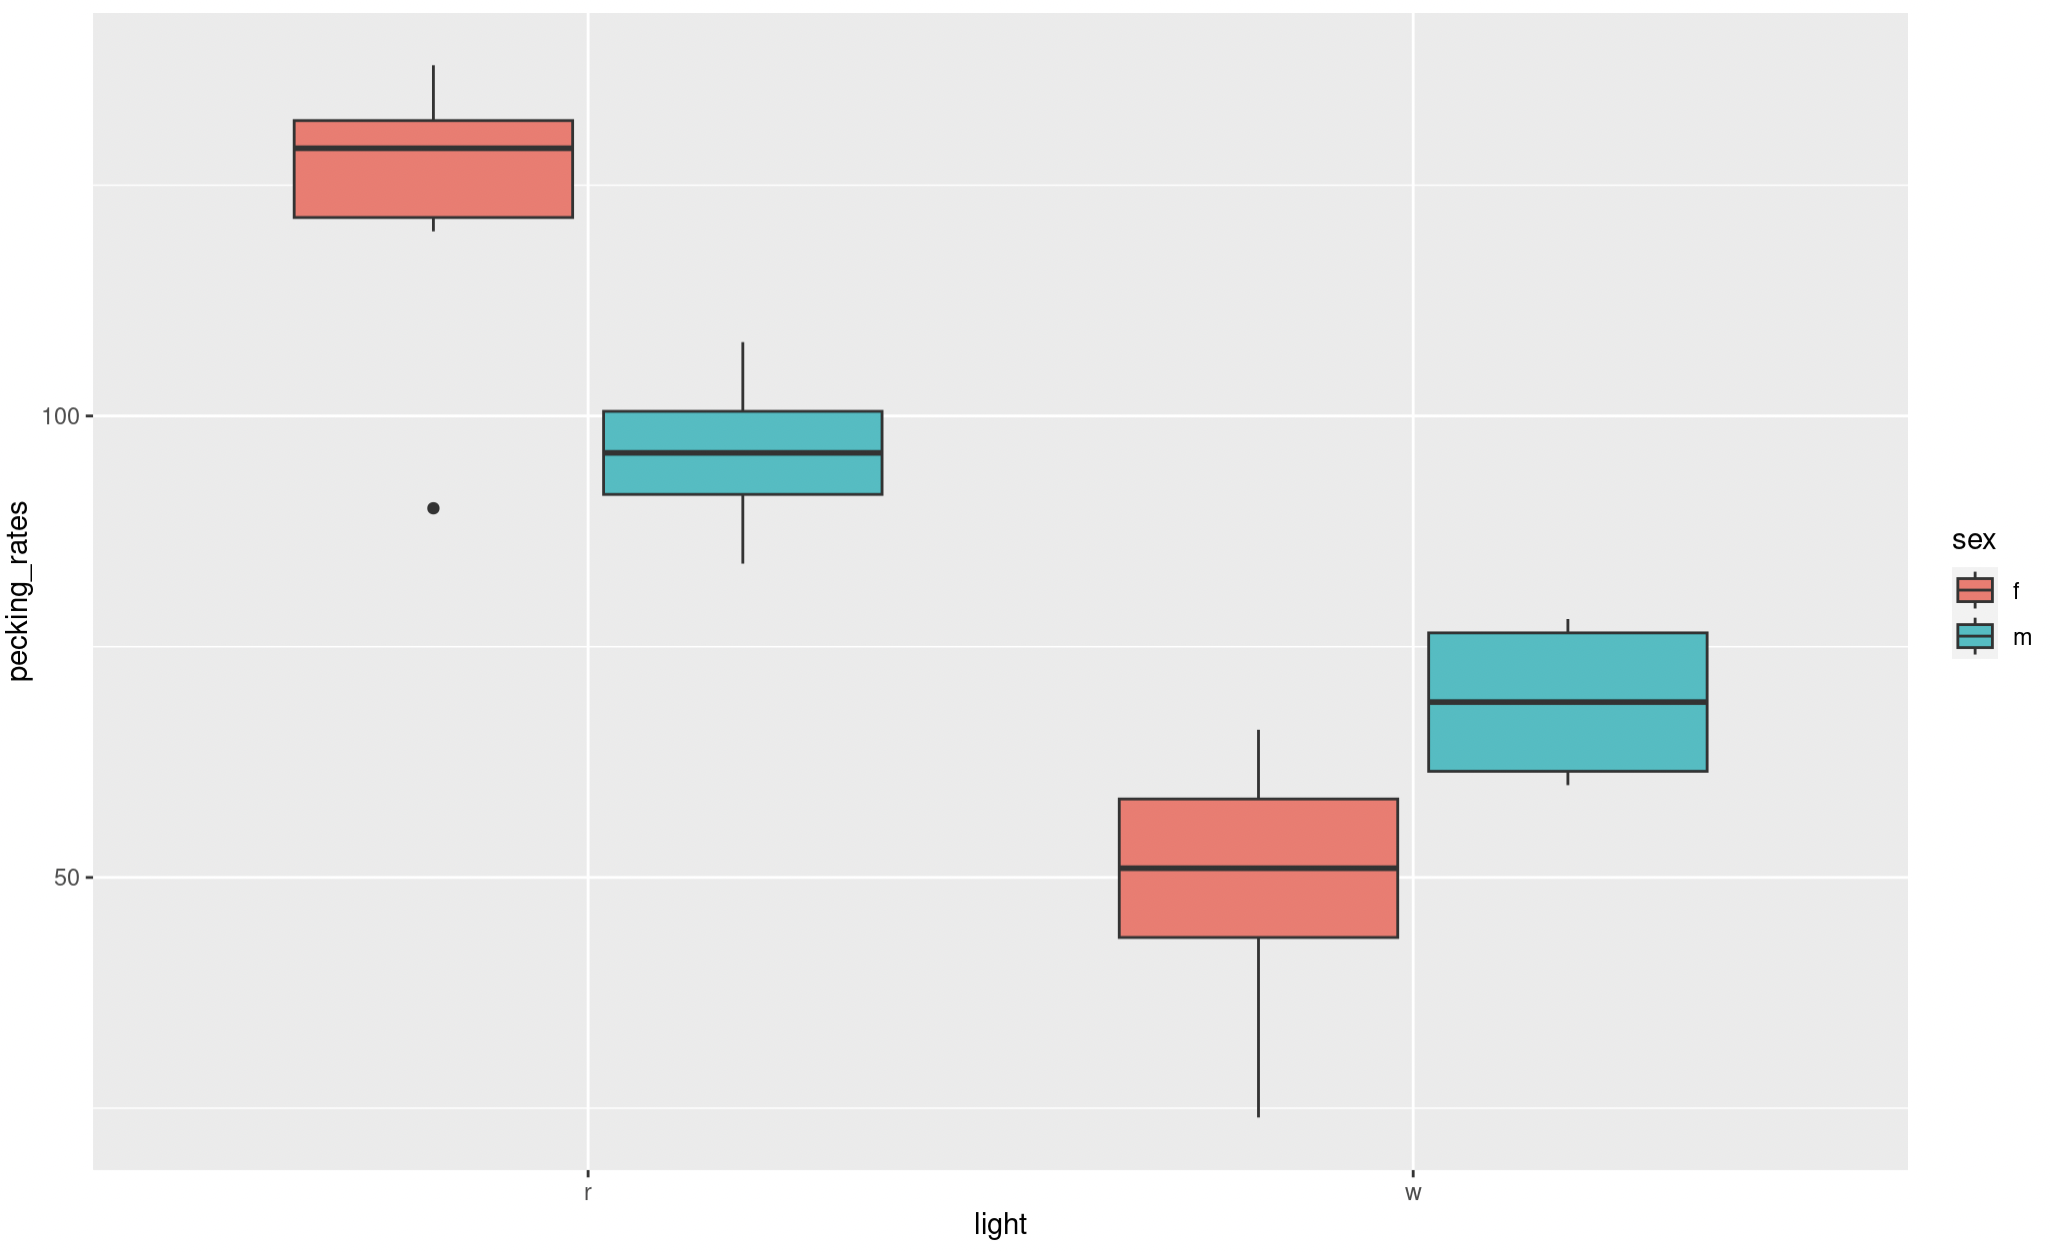
\includegraphics[width=0.9\linewidth]{figures/pecking_rates_2} \caption{A basic ggplot box plot output}\label{fig:unnamed-chunk-82}
\end{figure}

Have a look at this figure, is there anything you would change, to make it more visually appealing or clear?

Here are some things I would change:

\begin{itemize}
\tightlist
\item
  Labels
\item
  Colour scheme
\item
  Spacing
\item
  Theme
\end{itemize}

We will look into how to edit these elements now.

\hypertarget{labels}{%
\section{Labels}\label{labels}}

Clear accurate labeling is essential in the sciences, be it when your in the lab labeling up your samples or creating data visualisations.

In our current plot both our x and y axis could do with some relabeling, just because we dont use capitals when coding doesn't mean we don't follow the normal rules of English grammar when presenting data. Try adjusting your code so that it looks like the following;

\begin{Shaded}
\begin{Highlighting}[]
\CommentTok{\# Making a box plot and saving it in an object}
\CommentTok{\# Call the ggplot function and direct it to your data, define your x axis and y axis and colour your plots by sex}
\NormalTok{pecking\_rates\_box }\OtherTok{\textless{}{-}} \FunctionTok{ggplot}\NormalTok{(}\AttributeTok{data =}\NormalTok{ chickens,}\AttributeTok{aesdata =}\NormalTok{ chickens, }\FunctionTok{aes}\NormalTok{(}\AttributeTok{x =}\NormalTok{ light, }\AttributeTok{y =}\NormalTok{ pecking\_rates, }\AttributeTok{fill =}\NormalTok{ sex)) }\SpecialCharTok{+}
  \FunctionTok{geom\_boxplot}\NormalTok{() }\SpecialCharTok{+} \CommentTok{\# Tell ggplot that you want it to build a box plot}
  \FunctionTok{labs}\NormalTok{(}\AttributeTok{x =} \StringTok{"Light Colour"}\NormalTok{, }\AttributeTok{y =} \StringTok{"Number of Pecks (per 15 minutes) }\SpecialCharTok{\textbackslash{}n}\StringTok{"}\NormalTok{) }\CommentTok{\# Adjust your x and y axis labels}
\FunctionTok{print}\NormalTok{(pecking\_rates\_box) }\CommentTok{\# Print the object your plot is stored in to view it}
\end{Highlighting}
\end{Shaded}

Note the \texttt{\textbackslash{}n} on your y axis label. This simply adds a new line to the label and spaces it nicely away from the y axis.

This looks a bit better but our key is still not very well labeled. Adjust your \texttt{labs} function so that it reads \texttt{labs(x\ =\ "Light\ Colour",\ y\ =\ "Number\ of\ Pecks\ (per\ 15\ minutes)\ \textbackslash{}n",\ fill\ =\ "Sex")}. This will change the label for your key.

Our labels still aren't quite right, I don't like the abbreviations on the x axis and our key could still use some work as there are no units given for the treatment temperatures. Try these changes;

\begin{Shaded}
\begin{Highlighting}[]
\CommentTok{\# Making a box plot and saving it in an object}
\CommentTok{\# Call the ggplot function and direct it to your data, define your x axis and y axis and colour your plots by sex}
\NormalTok{pecking\_rates\_box }\OtherTok{\textless{}{-}} \FunctionTok{ggplot}\NormalTok{(}\AttributeTok{data =}\NormalTok{ chickens,}\AttributeTok{aesdata =}\NormalTok{ chickens, }\FunctionTok{aes}\NormalTok{(}\AttributeTok{x =}\NormalTok{ light, }\AttributeTok{y =}\NormalTok{ pecking\_rates, }\AttributeTok{fill =}\NormalTok{ sex)) }\SpecialCharTok{+}
  \FunctionTok{geom\_boxplot}\NormalTok{() }\SpecialCharTok{+} \CommentTok{\# Tell ggplot that you want it to build a box plot}
  \FunctionTok{labs}\NormalTok{(}\AttributeTok{x =} \StringTok{"Light Colour"}\NormalTok{, }\AttributeTok{y =} \StringTok{"Number of Pecks (per 15 minutes) }\SpecialCharTok{\textbackslash{}n}\StringTok{"}\NormalTok{, }\AttributeTok{fill =} \StringTok{"Sex"}\NormalTok{) }\SpecialCharTok{+} \CommentTok{\# Adjust your x and y axis labels as well as your key heading}
  \FunctionTok{scale\_x\_discrete}\NormalTok{(}\AttributeTok{labels =} \FunctionTok{c}\NormalTok{(}\StringTok{"Red"}\NormalTok{,}\StringTok{"White"}\NormalTok{)) }\SpecialCharTok{+} \CommentTok{\# Rename the categories on the x axis }
  \FunctionTok{scale\_fill\_manual}\NormalTok{(}\AttributeTok{labels =} \FunctionTok{c}\NormalTok{(}\StringTok{"Female"}\NormalTok{, }\StringTok{"Male"}\NormalTok{)) }\CommentTok{\# Rename your key labels}
\FunctionTok{print}\NormalTok{(pecking\_rates\_box) }\CommentTok{\# Print the object your plot is stored in to view it}
\end{Highlighting}
\end{Shaded}

Note that the \texttt{scale\ x\ discrete} and \texttt{scale\_fill\_manual} functions simply rename things in the same order as you present them, make sure you label your categories accurately or this can make a big mess later on.

If you try to remake your plot at this stage you will get the following error:

\begin{verbatim}
Error in `palette()`:
! Insufficient values in manual scale. 2 needed but only 0 provided.
Run `rlang::last_trace()` to see where the error occurred.
\end{verbatim}

This is because \texttt{scale\_fill\_manual} is also expecting some instructions on how to colour your boxplot. You will need to complete Chapter \ref{colours} before you can successfully remake your boxplot.

\hypertarget{colours}{%
\section{Switching up colours}\label{colours}}

The colours of your boxes are the default colours given by \texttt{ggplot()}. We can modify these to make our plot look a bit more pleasing. Try editing the \texttt{scale\_fill\_manual} function to this \texttt{scale\_fill\_manual(labels\ =\ c("Female",\ "Male"),\ values\ =\ c("cornflowerblue",\ "coral"))}. Run it and see what happens to your plot.

What do you think of your new plot now? Do you think the changes to labels and colours are an improvement?

R has lots of \href{https://www.datanovia.com/en/blog/awesome-list-of-657-r-color-names/}{colours}, take a look at the linked reference lists and have a play with changing up some of your colours.

Colour can be a really useful tool to employ when making your plots visually appealing, however make sure you are mindful that some colour pallets can be difficult for some people to interpret. There are however, some really good \href{https://www.tableau.com/en-gb/about/blog/examining-data-viz-rules-dont-use-red-green-together\#:~:text=Use\%20a\%20colour\%2Dblind\%2Dfriendly\%20palette\%20when\%20appropriate\&text=For\%20example\%2C\%20blue\%2Forange\%20is,blue\%20to\%20someone\%20with\%20CVD}{tips} out there for making sure your figures are accessible to everyone.

\hypertarget{spacing}{%
\section{Spacing}\label{spacing}}

Lets have a look at spacing. This is a box plot so we the main spacing option you are likely to want to play with is the width of your boxes. Here we can simply add an argument to the \texttt{geom\_boxplot()} function. Edit this function so that it reads \texttt{geom\_boxplot(width\ =\ 0.9)}. The width argument can be anything between 0.00 or 1.00. It changes the width of the boxes and this changes the spacing between them as well. Have a play with some values and see what happens.

We will come back to spacing when we look at our scatter plots later.

\hypertarget{themes}{%
\section{Themes}\label{themes}}

Another aspect of aesthetics that we can look at is themes. We have a reasonably attractive graph now, but its still got a grey background and the grid lines are unnecessary. To remove the grey background and implement the classic black on white aesthetic we can simply add a function that defines a pre-made theme. Adjust your script so that it includes the function \texttt{theme\_bw()}, I suggest you add this as a new line, don't forget to pipe between your functions with a \texttt{+}. Run this chunk and print your new plot. How is that looking now?

Two things still jump out at me when looking at this plot. The grid lines are completely unnecessary and detract from the overall aesthetic and the text sizes could be larger. To make these edits we can simply add additional instructions to adjust the theme further. So although most of the work has been done by applying a the \texttt{theme\_bw} we still need make some adjustments.

Add the following function to your growing ggplot chunk (don't forget to pipe \texttt{+} between functions);

\begin{Shaded}
\begin{Highlighting}[]
\FunctionTok{theme}\NormalTok{(}\AttributeTok{panel.border =} \FunctionTok{element\_rect}\NormalTok{(}\AttributeTok{color=}\StringTok{"black"}\NormalTok{), }\CommentTok{\# Specifies that the plot boarder is coloured black}
        \AttributeTok{panel.grid.minor =} \FunctionTok{element\_blank}\NormalTok{(), }\CommentTok{\# Removes minor grid lines }
        \AttributeTok{panel.grid.major =} \FunctionTok{element\_blank}\NormalTok{()) }\CommentTok{\# Removes major grid lines }
\end{Highlighting}
\end{Shaded}

Now we just need to adjust the text size. We can do this within the \texttt{theme} function as well adjust your theme so that it reads like this;

\begin{Shaded}
\begin{Highlighting}[]
\FunctionTok{theme}\NormalTok{(}\AttributeTok{panel.border =} \FunctionTok{element\_rect}\NormalTok{(}\AttributeTok{color=}\StringTok{"black"}\NormalTok{), }\CommentTok{\# Specifies that the plot boarder is coloured black}
        \AttributeTok{panel.grid.minor =} \FunctionTok{element\_blank}\NormalTok{(), }\CommentTok{\# Removes minor grid lines }
        \AttributeTok{panel.grid.major =} \FunctionTok{element\_blank}\NormalTok{(), }\CommentTok{\# Removes major grid lines }
        \AttributeTok{axis.text =} \FunctionTok{element\_text}\NormalTok{(}\AttributeTok{size =} \DecValTok{15}\NormalTok{), }\CommentTok{\# Changes the size of text on both axis }
        \AttributeTok{axis.title =} \FunctionTok{element\_text}\NormalTok{(}\AttributeTok{size =} \DecValTok{20}\NormalTok{), }\CommentTok{\# Changes size of your axis labels }
        \AttributeTok{legend.text =} \FunctionTok{element\_text}\NormalTok{(}\AttributeTok{size =} \DecValTok{15}\NormalTok{), }\CommentTok{\# Changes the size of text within your legend}
        \AttributeTok{legend.title =} \FunctionTok{element\_text}\NormalTok{(}\AttributeTok{size =} \DecValTok{20}\NormalTok{)) }\CommentTok{\# Changes the size of the legend title}
\end{Highlighting}
\end{Shaded}

Have a play with the different text sizes until you think they are optimal. You may need to press the zoom button in the viewer panel to get a clearer idea of the scaling.

Hopefully you now have a nice clean, clear and aesthetically pleasing plot and have some awareness of the commands and functions used to make it.

\hypertarget{beautifying-scatter-plots}{%
\section{Beautifying scatter plots}\label{beautifying-scatter-plots}}

In Chapter \ref{c6t2} and \ref{c6t3} we made a very simple scatter plot for radiation exposure against cancer mortality (deaths per 100,000 person-years, 1959-1964) across nine counties in the US. Reopen your script from this workshop, recreate the accompanying data frame and rebuilt your \texttt{geom\_point()} plot.

Use you previous chunks of code and knowledge of R to edit the labels and themes of this plot. Print it again and take a look.

Now there are some additional elements in this plot that could be adjusted. These include;

\begin{itemize}
\tightlist
\item
  Point shape - The shape of the individual points on the plot, as with colours there are lots of options numbered 0 - 25, descriptions of each one are listed here
\item
  Point size - The size of each point
\item
  Point colour - The colour of your points
\item
  Line type (solid, dashed, etc) - Again thre are several options here, the notation and descriptions of which can be found here
\item
  Line colour
\item
  Line size - the weight of the line
\item
  Line fill - Note that here this refers to the colour of the shaded area marking the standard error
\end{itemize}

So lets play with some of these. Try adding and adjusting the following arguments within \texttt{geom\_point()}

\begin{itemize}
\tightlist
\item
  \texttt{shape\ =\ 1} - have a look at other point shapes you could use and play with this setting
\item
  \texttt{size\ =\ 2} - again try playing with some point sizes
\item
  \texttt{colour\ =\ "blue"} - or any other colour you fancy trying.
\end{itemize}

Once you are happy with your points we can take a look at your regression line. Try adding and adjusting the following arguments within \texttt{geom\_smooth()}

\begin{itemize}
\tightlist
\item
  \texttt{colour\ =\ "cornflowerblue"}
\item
  \texttt{fill\ =\ "lightblue"}
\item
  \texttt{size\ =\ 1}
\item
  \texttt{linetype\ =\ "dashed"}
\end{itemize}

As before please do experiment and play with the settings described by each of these arguments.

\hypertarget{explorting-your-plot-to-pdf}{%
\section{Explorting your plot to pdf}\label{explorting-your-plot-to-pdf}}

Once you are happy with your new and beautiful plots make sure you save it to to the figures folder using a function called \texttt{ggsave()}. This will allow you to export your plots as \texttt{.pdf} files which you can then download and put in your reports/publications.

You will need to have your plots saved as an object (using the \texttt{\textless{}-} syntax) before this will work. You can call these objects whatever makes most sense to you. Try running the code below for each of your beautified plots;

\begin{Shaded}
\begin{Highlighting}[]
\CommentTok{\# Saving outputs}
\FunctionTok{ggsave}\NormalTok{(}\StringTok{"figures/pecking\_rates\_boxplot.pdf"}\NormalTok{, }\CommentTok{\# Give R a path to save to and a file name}
       \AttributeTok{plot =}\NormalTok{ pecking\_rates\_box,}\CommentTok{\# Tell R what to save {-} in this case your object}
       \AttributeTok{width =} \DecValTok{15}\NormalTok{, }\CommentTok{\# Set .pdf width}
       \AttributeTok{height =} \DecValTok{10}\NormalTok{, }\CommentTok{\# Set .pdf height}
       \AttributeTok{units =} \StringTok{"cm"}\NormalTok{, }\CommentTok{\# Specify units for .pdf width and height}
       \AttributeTok{device =} \StringTok{"pdf"}\NormalTok{) }\CommentTok{\# Tell R what file type to create, in this case a pdf}
\CommentTok{\# Note, use trial and error to select a good width and height for your figure}
\end{Highlighting}
\end{Shaded}

Note that if you remove the \texttt{device\ =} line \texttt{ggsave} will automatically create a \texttt{.png} file. You can also use \texttt{width\ =\ ,\ height\ =\ ,\ units\ =\ "cm"} arguments to specify the size of your figure in cm. You will need to adjust these by trial and error until the proportional sizing of your plot to axis and legend labels is pleasing. This chunk will save your plot to the \texttt{figures} folder. From here you can download your figures by checking the box besides the file, clicking \texttt{More} and then \texttt{Export...} and \texttt{Download}.

\hypertarget{before-you-leave-7}{%
\section{Before you leave!}\label{before-you-leave-7}}

Make sure you save your script and download it if you would like to keep a local copy.

Please log out of posit Cloud!

\hypertarget{references-6}{%
\section{References}\label{references-6}}

Wickham, Hadley, Mara Averick, Jennifer Bryan, Winston Chang, Lucy D'Agostino McGowan, Romain François, Garrett Grolemund, et al.~2019. ``Welcome to the tidyverse.'' Journal of Open Source Software 4 (43): 1686. \url{https://doi.org/10.21105/joss.01686}.
Wickham, Hadley, Winston Chang, Lionel Henry, Thomas Lin Pedersen, Kohske Takahashi, Claus Wilke, Kara Woo, Hiroaki Yutani, and Dewey Dunnington. 2021. Ggplot2: Create Elegant Data Visualisations Using the Grammar of Graphics. \url{https://CRAN.R-project.org/package=ggplot2}.

\hypertarget{bio-7026a-univariate-statistics-summative-assignment}{%
\chapter{BIO-7026A: Univariate Statistics Summative Assignment}\label{bio-7026a-univariate-statistics-summative-assignment}}

Report Length: 2000 words (maximum)

\hypertarget{the-exercise}{%
\section{The exercise}\label{the-exercise}}

There are \textbf{two} separate parts to this assignment:

\begin{itemize}
\tightlist
\item
  \textbf{Part 1:} for each of the five questions below, describe (a) the test you selected (b) why that test is appropriate and (c) the procedures you followed to conduct and interpret each test.
\item
  \textbf{Part 2:} present the results of your analyses in the style of the results section of a scientific paper.
\end{itemize}

\hypertarget{the-problem}{%
\section{The Problem}\label{the-problem}}

The kooki bird is a very rare (fictional) species, which now exists only on a few islands. The birds are largely frugivorous, and natural fruit yield on the islands can vary with weather conditions. Since 1980, a captive breeding programme has been in place and chick productivity has been measured for both captive birds and birds breeding in the wild. Weather data have also been measured at a local meteorological station. The investigators are interested in assessing how maximum daytime temperatures during September and October and rainfall during January and February might affect wild chick productivity. The length of the breeding season was also recorded as the (standardised) number of days during which the temperature reached 15°C. The data table below gives the mean chick productivity for wild and captive birds, and the weather and breeding season length in each year.

In addition to this, on the largest island, a long-term experiment was set up to examine the effects of different levels of supplemental feeding with bananas and mangos. There are two levels of banana and mango supplementation (none vs the standard supplement of 100 g bird\(^-\)\(^1\)). The experiment is a fully factorial design, with each of the four treatment combinations occurring in each year, and the arrangement of the experimental feeders on the island is fully randomized. As the birds are highly sedentary, they only experience the food supplementation at the feeder nearest them. The data table below gives the mean chick productivity for the pairs experiencing each treatment within each year.

Using whatever statistical analyses you feel appropriate, answer the following questions;

\begin{enumerate}
\def\labelenumi{\arabic{enumi})}
\tightlist
\item
  How does chick productivity of wild birds compare to that of the captive birds?
\item
  Is there any evidence for changes in productivity over the study period among the wild birds?\\
\item
  Is there evidence of the weather variables influencing chick productivity among the wild birds?
\item
  Does chick productivity of wild birds vary with the length of the breeding season?
\item
  What are the effects of the food supplementation treatments on kooki bird productivity?
\end{enumerate}

\textbf{Hints \& Tips}

\begin{itemize}
\tightlist
\item
  The data presented below will, in places, need reformatting before you will be able to conduct your analysis.
\item
  For good examples of how results of analyses should be presented and described, consult Results sections of publications in a scientific journal, such as Journal of Animal Ecology or Journal of Applied Ecology. Part 2 of the assignment should be presented in this style.
\item
  Don't be tempted to use multivariate techniques to analyse the effects of weather on productivity -- use only the analytical approaches covered in this module.
\end{itemize}

Put your responses to \textbf{Part 1} and \textbf{Part 2} in a word document. You will be able to submit your work through the BIO-7026A page on Blackboard.

\hypertarget{the-data-3}{%
\section{The Data}\label{the-data-3}}

\begin{longtable}[]{@{}
  >{\centering\arraybackslash}p{(\columnwidth - 22\tabcolsep) * \real{0.0833}}
  >{\centering\arraybackslash}p{(\columnwidth - 22\tabcolsep) * \real{0.0833}}
  >{\centering\arraybackslash}p{(\columnwidth - 22\tabcolsep) * \real{0.0833}}
  >{\centering\arraybackslash}p{(\columnwidth - 22\tabcolsep) * \real{0.0833}}
  >{\centering\arraybackslash}p{(\columnwidth - 22\tabcolsep) * \real{0.0833}}
  >{\centering\arraybackslash}p{(\columnwidth - 22\tabcolsep) * \real{0.0833}}
  >{\centering\arraybackslash}p{(\columnwidth - 22\tabcolsep) * \real{0.0833}}
  >{\centering\arraybackslash}p{(\columnwidth - 22\tabcolsep) * \real{0.0833}}
  >{\centering\arraybackslash}p{(\columnwidth - 22\tabcolsep) * \real{0.0833}}
  >{\centering\arraybackslash}p{(\columnwidth - 22\tabcolsep) * \real{0.0833}}
  >{\centering\arraybackslash}p{(\columnwidth - 22\tabcolsep) * \real{0.0833}}
  >{\centering\arraybackslash}p{(\columnwidth - 22\tabcolsep) * \real{0.0833}}@{}}
\toprule\noalign{}
\begin{minipage}[b]{\linewidth}\centering
Wild birds \(^1\)
\end{minipage} & \begin{minipage}[b]{\linewidth}\centering
Captive-bred birds \(^1\)
\end{minipage} & \begin{minipage}[b]{\linewidth}\centering
BO MO \(^2\)
\end{minipage} & \begin{minipage}[b]{\linewidth}\centering
B1 MO \(^2\)
\end{minipage} & \begin{minipage}[b]{\linewidth}\centering
B0 M1 \(^2\)
\end{minipage} & \begin{minipage}[b]{\linewidth}\centering
B1 M1 \(^2\)
\end{minipage} & \begin{minipage}[b]{\linewidth}\centering
Jan Rain (cm) \(^3\)
\end{minipage} & \begin{minipage}[b]{\linewidth}\centering
Feb Rain (cm) \(^3\)
\end{minipage} & \begin{minipage}[b]{\linewidth}\centering
Sept Temp (°C) \(^4\)
\end{minipage} & \begin{minipage}[b]{\linewidth}\centering
Oct Temp (°C) \(^4\)
\end{minipage} & \begin{minipage}[b]{\linewidth}\centering
Breeding Period (Standardised) \(^5\)
\end{minipage} & \begin{minipage}[b]{\linewidth}\centering
\end{minipage} \\
\midrule\noalign{}
\endhead
\bottomrule\noalign{}
\endlastfoot
0.54 & 0.04 & 0.54 & 0.73 & 0.56 & 0.73 & 2.30 & 2.30 & 15.05 & 18 & -0.52 & \\
0.55 & 0.02 & 0.53 & 0.64 & 0.54 & 0.68 & 2.40 & 2.10 & 16.1 & 17.55 & 0.13 & \\
0.58 & 0.04 & 0.61 & 0.71 & 0.61 & 0.72 & 1.90 & 1.10 & 17.4 & 17.5 & 0.39 & \\
0.50 & 0.02 & 0.49 & 0.64 & 0.51 & 0.71 & 2.20 & 3.50 & 16.55 & 18.35 & -0.02 & \\
0.49 & 0.02 & 0.45 & 0.52 & 0.48 & 0.60 & 2.20 & 1.90 & 13.05 & 17.5 & -0.17 & \\
0.41 & 0.06 & 0.32 & 0.34 & 0.33 & 0.38 & 1.50 & 1.40 & 13.1 & 14.85 & -1.72 & \\
0.32 & 0.03 & 0.45 & 0.46 & 0.48 & 0.63 & 1.10 & 1.70 & 14.65 & 17.4 & -0.37 & \\
0.33 & 0.50 & 0.44 & 0.52 & 0.51 & 0.57 & 1.10 & 0.80 & 16.85 & 18.05 & 0.08 & \\
0.54 & 0.33 & 0.54 & 0.62 & 0.57 & 0.63 & 1.50 & 0.80 & 16.45 & 17 & 0.29 & \\
0.35 & 0.62 & 0.36 & 0.46 & 0.40 & 0.52 & 1.10 & 2.50 & 15.65 & 18.15 & 0.42 & \\
0.26 & 0.10 & 0.29 & 0.35 & 0.33 & 0.42 & 0.60 & 0.40 & 14.45 & 18.1 & -1.57 & \\
0.38 & 0.01 & 0.35 & 0.38 & 0.45 & 0.46 & 0.90 & 0.70 & 14.6 & 17.95 & -0.02 & \\
0.22 & 0.02 & 0.41 & 0.50 & 0.47 & 0.60 & 0.20 & 4.20 & 16.75 & 17.1 & -0.77 & \\
0.46 & 0.08 & 0.31 & 0.58 & 0.34 & 0.60 & 1.80 & 1.80 & 16.65 & 16.3 & 0.34 & \\
0.43 & 0.13 & 0.43 & 0.56 & 0.46 & 0.63 & 0.50 & 2.00 & 14.65 & 17.9 & -0.97 & \\
0.57 & 0.81 & 0.41 & 0.52 & 0.42 & 0.68 & 2.10 & 1.10 & 14.9 & 18.45 & 0.03 & \\
0.40 & 0.06 & 0.50 & 0.64 & 0.52 & 0.62 & 1.50 & 1.00 & 18 & 17.45 & -0.12 & \\
0.53 & 0.09 & 0.51 & 0.60 & 0.59 & 0.80 & 0.80 & 1.60 & 16.1 & 18.35 & -1.17 & \\
0.36 & 0.09 & 0.36 & 0.37 & 0.58 & 0.46 & 1.10 & 0.30 & 16.4 & 17.1 & -1.72 & \\
0.38 & 0.03 & 0.35 & 0.48 & 0.42 & 0.46 & 0.50 & 1.40 & 14.5 & 17.35 & -1.67 & \\
0.45 & 0.16 & 0.59 & 0.55 & 0.59 & 0.67 & 1.30 & 1.60 & 14.6 & 18.65 & 0.49 & \\
0.51 & 0.01 & 0.54 & 0.68 & 0.59 & 0.71 & 2.10 & 2.80 & 15 & 16.2 & 0.89 & \\
0.65 & 0.05 & 0.45 & 0.77 & 0.41 & 0.67 & 2.30 & 3.50 & 13.5 & 20.3 & 0.54 & \\
0.63 & 0.03 & 0.55 & 0.84 & 0.58 & 0.97 & 2.70 & 1.60 & 16 & 18.2 & 1.44 & \\
0.58 & 0.01 & 0.59 & 0.57 & 0.71 & 0.77 & 1.20 & 1.20 & 17.8 & 16.4 & 1.74 & \\
0.52 & 0.02 & 0.56 & 0.61 & 0.53 & 0.57 & 0.70 & 0.90 & 18.45 & 18.3 & 1.79 & \\
0.44 & 0.02 & 0.45 & 0.51 & 0.56 & 0.56 & 0.90 & 1.00 & 17.95 & 17.85 & 1.04 & \\
0.53 & 0.05 & 0.55 & 0.66 & 0.63 & 0.79 & 1.60 & 1.80 & 17.4 & 18.7 & 0.69 & \\
0.69 & 0.07 & 0.50 & 0.82 & 0.51 & 0.77 & 2.70 & 1.80 & 16.6 & 19.9 & 1.34 & \\
\end{longtable}

\(^1\) Mean no. of chicks per pair of wild and captive birds each year (1980 onwards)
\(^2\) Chick no's per pair in each of the four food treatments (banana supplement (B1), mango supplement (M1) and no supplement (B0 and M0)) in each year
\(^3\) Total rainfall in January and February of each year
\(^4\) Mean temperature in September and October of each year
\(^5\) Standardised length of the breeding season (difference from long-term average)

\hypertarget{introduction-to-multivariate-statistics-bio-7025a}{%
\chapter{Introduction to Multivariate Statistics (BIO-7025A)}\label{introduction-to-multivariate-statistics-bio-7025a}}

\hypertarget{welcome-to-multivairate-statistics}{%
\section{Welcome to Multivairate Statistics}\label{welcome-to-multivairate-statistics}}

In this second 10 credit module we will be following on from the concepts, skills and techniques we learned before in Univariate statistics (BIO-7026A). The next few chapters will cover;

\begin{itemize}
\tightlist
\item
  Multiple Linear Regressions - Week 8
\item
  Model Structure, Mixed Multiple Linear Regressions and Repeated Linear Models - Week 9
\item
  Generalised Linear Models - Week 10
\end{itemize}

After this point Dr Richard Davies will take over and over Weeks 11 and 12 will cover;

\begin{itemize}
\tightlist
\item
  Principal Component Analysis
\item
  Multivariate Community Analysis
\end{itemize}

As this module builds on many of the skills from Univariate Statistics, you may find that you need to look back and remind yourselves of techniques and code from former chapters or scripts. Don't be afraid to do this.

\hypertarget{learning-objectives-1}{%
\section{Learning Objectives}\label{learning-objectives-1}}

\begin{itemize}
\tightlist
\item
  To introduce students to the statistical framework of General Linear Modelling, combining linear regression, ANOVA and ANCOVA into a single technique
\item
  Learn binary logistic regression, ordination and Principal Components Analysis
\item
  Review issues in experimental and sampling design and the assumptions underlying general linear models and the principal model simplification
\item
  To learn to run these tests using R and to interpret and present the results
\end{itemize}

\hypertarget{teaching-layout-1}{%
\section{Teaching Layout}\label{teaching-layout-1}}

This is a 10 credit module which will run from Weeks 8 - 12.

\begin{itemize}
\tightlist
\item
  Each week will have two three hour practical sessions in IT labs (Mondays and Fridays).
\item
  Some of the following chapters will be completed in a single three hour workshop, others will span both workshops.
\item
  Each chapter will be accompanied by a mini lecture at the start of the corresponding workshop.
\end{itemize}

\hypertarget{multivariate-linear-modelling}{%
\chapter{Multivariate Linear Modelling}\label{multivariate-linear-modelling}}

This chapter will run over both workshops (6/7) in Week 8.

\hypertarget{introduction-5}{%
\section{Introduction}\label{introduction-5}}

Multivariate linear modelling techniques are used when entering more than one predictor (independent variable) into an analysis of a dependent variable (also called response variable). The process and much of the output are very similar to those of simple linear regression, in which the effect of just one predictor is assessed. The aim is to explain the variance in the dependent variable, just as in simple regression, but with multiple predictor variables. Each of the predictor variables may explain a unique part of the variance in the dependent variable, but they may also share some of the variance that they explain.

The form of a multiple regression equation is an extension of that in simple regression:

\[
y = m_1x_1+m_2x_2+m_3x_3...+c
\]

and the statistical analysis is also in the form of ANOVA and t-tests of each parameter.

\begin{enumerate}
\def\labelenumi{\arabic{enumi})}
\tightlist
\item
  Multiple regression can be greatly influenced by which predictors are included, so it is important to not just throw in any old predictor; there should be a biological hypothesis attached to each predictor that is included.
\item
  The default option for how predictions are entered into models is \textbf{Enter}: all predictors are entered simultaneously and the researcher can then choose to exclude non-significant variables (this is often called a step-down method).
\item
  In general with multiple regression, the fewer predictors the better, and you should have a minimum of 10-15 data points per predictor (or your model is unlikely to have sufficient power to identify relationships, should they exist)
\item
  Assumptions: even distribution of residuals, no heteroscedasticity and avoid collinearity of predictors (particularly when the correlation coefficient r \textgreater{} 0.7).
\end{enumerate}

In a linear model, you have three ways of entering a predictor variable:

\begin{itemize}
\tightlist
\item
  \textbf{Covariates:} continuous predictor variables are entered as covariates
\item
  \textbf{Fixed factors:} these are categorical predictor variables for which you want to compare the different categories.
\item
  \textbf{Random factors:} these are categorical variables that need to be included in the model but for which you don't want to compare the categories. Random factors are often included to account for some non-independence in your data (eg multiple datapoints from the same site or year).
\end{itemize}

\textbf{You MUST NOT include both fixed and random effects in the same linear model -- for that you have to use a MIXED MODEL}

\hypertarget{practical-6---multiple-linear-models}{%
\section{Practical 6 - Multiple Linear Models}\label{practical-6---multiple-linear-models}}

This week we will be analysing three separate data sets; Africa, chaffinch and beetle. You can find these in our new classroom click \href{https://posit.cloud/spaces/445363/join?access_code=FJxK_vnNriot52seLUoKS-fpSCL4Z59m5vRW6d1d}{here}. Try to pay special attention to the data interpretation steps and make sure you understand the logic behind each of the decisions made.

Once you have joined the classroom, spend some time setting up your workspace and script as covered in Chapter \ref{workspace-setup} and Chapter \ref{script-setup}. You will need to install and load the packages \texttt{tidyverse} and \texttt{janitor} for this weeks sessions.

\hypertarget{data-set-1-africa}{%
\section{Data set 1: Africa}\label{data-set-1-africa}}

Here you will be analysing data from 34 sub-Saharan African nations, collected by the World Bank in 1985. The aim is to fit a model that can be used to predict per capita calorific intake rate and to examine, from a conservation perspective, how deforestation impacts on calorific intake.

The variables are:

Dependent Variable: Possible Predictor Variables:

\begin{itemize}
\tightlist
\item
  daycal: per capita daily calorific intake
\item
  femlit: female illiteracy rate (for over 15s)
\item
  under15: percentage of the population under 15
\item
  deforest: annual rate of forest loss
\item
  gnp: per capita Gross National Daily Product (US \$)
\end{itemize}

Theories have been suggested that poor diet, as represented by low calorific intake, is more serious in countries with poor economies, lower levels of education, a young population, and high levels of deforestation. In this practical, try to assess whether such relationships exist.

\hypertarget{task-1---checking-the-data}{%
\subsection{Task 1 - Checking the data}\label{task-1---checking-the-data}}

Load the dataset \texttt{africa.csv} into your workspace under the object name \texttt{africa} and try performing some routine checks to make sure R has interpreted the variables correctly and all expected data is present and accounted for. You can use some of the functions explored in Chapter \ref{checking-the-data} if you need some help with this.

\hypertarget{task-2---exploring-the-data}{%
\subsection{Task 2 - Exploring the data}\label{task-2---exploring-the-data}}

Start by exploring the univariate relationship between per capita daily calorific intake and gross national product.

\begin{quote}
\begin{itemize}
\tightlist
\item
  Write down what question you are asking, and turn this into a word equation (i.e.~y = mx + c, with symbols replaced by words).
\end{itemize}
\end{quote}

Draw the scatterplot for the relationship between per capita daily calorific intake (daycal) and gross national product (gnp), revisit Chapter \ref{c6t2} if you're not sure how to do this.

\begin{quote}
\begin{itemize}
\tightlist
\item
  Does the graph suggest that the assumptions of linear regression (i.e.~that all datapoints are contributing similarly to the slope) have been met?
\end{itemize}
\end{quote}

\hypertarget{task-3---regression-analysis}{%
\subsection{Task 3 - Regression analysis}\label{task-3---regression-analysis}}

Try running a linear regression for daily calorific intake and gross national product, store your model under the object name \texttt{daycal\_gnp\_lm\_1} revisit Chapter \ref{c6t3} if you're not sure how to do this.

\begin{quote}
\begin{itemize}
\tightlist
\item
  What does the regression model output tell you about the relationship between calorific intake and GNP?
\item
  Write down what the slope, constant, r\(^2\) and p-value tell you about this relationship, and consider whether they accurately describe this relationship.
\end{itemize}
\end{quote}

As we did in Chapter \ref{c6t3}, try plotting the residuals against the predicted values.

\begin{quote}
\begin{itemize}
\tightlist
\item
  From this plot, have the assumptions of the linear regression been met?
\end{itemize}
\end{quote}

We can also calculate leverage values, this measures the influence of each point on the fit of the regression and can range from 0: no influence to 1: complete influence. Try running the following;

\begin{Shaded}
\begin{Highlighting}[]
\CommentTok{\# Checking the leverage }
\NormalTok{africa }\OtherTok{\textless{}{-}}\NormalTok{ africa }\SpecialCharTok{\%\textgreater{}\%}
  \FunctionTok{mutate}\NormalTok{(}\AttributeTok{leverage =} \FunctionTok{hatvalues}\NormalTok{(daycal\_gnp\_lm\_1))}
\end{Highlighting}
\end{Shaded}

\begin{quote}
\begin{itemize}
\tightlist
\item
  What do the leverage values indicate?
\item
  Are any countries not fitting the model well?
\end{itemize}
\end{quote}

Try performing a log10 transformation on the gnp variable, revisit Chapter \ref{c7t3} if you unsure how to do this. Then re-run the regression model using the logged variable, and redraw the scatterplot

\begin{quote}
\begin{itemize}
\tightlist
\item
  Has the model fit improved? Compare the slope, intercept, r\(2\) and p-value to the model with the unlogged GNP.
\end{itemize}
\end{quote}

Have a look at the leverage values and the residuals for your new model. Country 11 (Gabon) still has something of a disproportionate effect on the fit of the regression line (large-ish leverage), even in the model with log (GNP). Use the following command to temporarily exclude this country from our scatter plot (note we are not deleting the data completely). This will allow you to explore the influence of Gabon.

\begin{Shaded}
\begin{Highlighting}[]
\NormalTok{africa }\SpecialCharTok{\%\textgreater{}\%}
  \FunctionTok{filter}\NormalTok{(name }\SpecialCharTok{!=} \StringTok{"Gabon"}\NormalTok{) }\SpecialCharTok{\%\textgreater{}\%}
  \FunctionTok{ggplot}\NormalTok{(}\AttributeTok{data =}\NormalTok{ ., }\FunctionTok{aes}\NormalTok{(}\AttributeTok{x =}\NormalTok{ gnp, }\AttributeTok{y =}\NormalTok{ daycal)) }\SpecialCharTok{+}
  \FunctionTok{geom\_point}\NormalTok{() }\SpecialCharTok{+}
  \FunctionTok{geom\_smooth}\NormalTok{(}\AttributeTok{method =}\NormalTok{ lm)}
\end{Highlighting}
\end{Shaded}

Now use the same temporary exclusion method to re-run your regression model with Gabon temporarily excluded.

\begin{quote}
\begin{itemize}
\tightlist
\item
  How has the regression changed? What reasons may there be for omitting Gabon from the analysis? Why should you always be careful when dropping variables for this reason?
\end{itemize}
\end{quote}

Re-include Gabon into subsequent analyses.

\hypertarget{c11t4}{%
\subsection{Task 4 - Multivariate linear regression analysis}\label{c11t4}}

We are now going to build a multivariate regression model using the Enter method, in which we begin by including all predictor variables in our regression. We then remove from our regression the variable that has the least (statistically non-significant) effect to produce a better model. We repeat this until we are left with a regression containing the best sub-set of predictors. At each stage it is important to consider the impact of removing that predictor on the model.
First we will draw a matrix plot to compare all of the relationships between \texttt{daycal} and all four predictor variables (use your logged gnp variable to reduce difficulties with Gabon). Try using the following command;

\begin{Shaded}
\begin{Highlighting}[]
\CommentTok{\# Scatter matrix}
\FunctionTok{pairs}\NormalTok{(africa[,}\FunctionTok{c}\NormalTok{(}\DecValTok{3}\SpecialCharTok{:}\DecValTok{7}\NormalTok{,}\DecValTok{9}\NormalTok{)])}
\CommentTok{\# Note the numbers c(3:7,9) refer to column numbers for daycal, femlit, under15, deforest and log10\_gnp they may be different in your data set}
\end{Highlighting}
\end{Shaded}

\begin{quote}
\begin{itemize}
\tightlist
\item
  Write down what these graphs tell you about each of the relationships
\item
  Do you see any signs of collinearity between predictor variables?
\end{itemize}
\end{quote}

Now we can try fitting the full multiple regression by adding the other three predictors as independent variables with Enter as the data entry method. Try running the following;

\begin{Shaded}
\begin{Highlighting}[]
\CommentTok{\# multiple regression}
\NormalTok{daycal\_multi\_lm\_1 }\OtherTok{\textless{}{-}} \FunctionTok{lm}\NormalTok{(daycal}\SpecialCharTok{\textasciitilde{}}\NormalTok{gnp}\SpecialCharTok{+}\NormalTok{deforest}\SpecialCharTok{+}\NormalTok{under15}\SpecialCharTok{+}\NormalTok{femlit, }\AttributeTok{data =}\NormalTok{ africa)}
\FunctionTok{summary}\NormalTok{(daycal\_multi\_lm\_1)}
\end{Highlighting}
\end{Shaded}

\begin{quote}
\begin{itemize}
\tightlist
\item
  Which is the most statistically significant variable?
\end{itemize}
\end{quote}

Remove the non-significant variable with the highest p-value from the regression model and examine the change in the adjusted \(r^2\).

\begin{quote}
\begin{itemize}
\tightlist
\item
  Has removing the variable altered the explanatory power of the regression (check the adjusted r\(^2\) now we are working with mulivariate linear models) very much? What has happened to the coefficients (slopes) of the remaining variables?
\end{itemize}
\end{quote}

By removing the least significant variable at each stage, you reduce the regression equation until it only contains significant variables (this is called the minimum model). At each stage, check that removing a predictor variable does not cause the r\(^2\) of the model to drop too much or cause the sign of the slope coefficient or the significance of other variables in the model to change strongly.

\begin{quote}
\begin{itemize}
\tightlist
\item
  Look at your final model. How does the r\(^2\) compare with the r\(^2\) you obtained in exercise 1, using simple regression with log(GNP) as the sole predictor?
\item
  Does your final model fit in with the original hypotheses about daily calorific intake?
\item
  What are the agreements and disagreements between your model and the theory (look back at the suggestions listed at the start of the practical)? Looking at the coefficients may be useful here.
\item
  Write a word equation for your final model.
\item
  Use your final model to predict the expected per capita calorific intake rate for a country with a GNP of US \$975, a female illiteracy rate of 45\% and a deforestation rate of -2.0.
\end{itemize}
\end{quote}

R has a function called \texttt{predict()} which can be used to predict values of y based on your model. Try runnign the following;

\begin{Shaded}
\begin{Highlighting}[]
\NormalTok{new }\OtherTok{\textless{}{-}} \FunctionTok{data.frame}\NormalTok{(}\AttributeTok{gnp =}\DecValTok{975}\NormalTok{, }\AttributeTok{femlit =}\DecValTok{45}\NormalTok{, }\AttributeTok{deforest=} \SpecialCharTok{{-}}\DecValTok{2}\NormalTok{)}
\CommentTok{\# Create a new data frame called \textasciigrave{}new\textasciigrave{} and specify your independent variable values}

\FunctionTok{predict}\NormalTok{(enter\_your\_final\_model\_here, }\AttributeTok{newdata=}\NormalTok{new, }\AttributeTok{interval =} \StringTok{\textquotesingle{}confidence\textquotesingle{}}\NormalTok{)}
\CommentTok{\# Call the predict function to use your final multivariate linear model to predict the daycal value in a country with the independent variable values specified in your data frame called \textasciigrave{}new\textasciigrave{}}
\CommentTok{\# By including interval = \textquotesingle{}confidence\textquotesingle{} the output will include 95\% confidence intervals.}
\end{Highlighting}
\end{Shaded}

\begin{quote}
\begin{itemize}
\tightlist
\item
  Compare the daycal rate you predicted for a country with a GNP of US \$975, a female illiteracy rate of 45\% and a deforestation rate of -2.0 to that predicted by the \texttt{predict()} function in R.
\item
  Does the 95\% prediction interval lie above or below the minimum acceptable daily calorific intake rate of 2000 kcal? What does this mean for this hypothetical country?
\end{itemize}
\end{quote}

You can also specify interactions to test using the \texttt{lm()} function by using a \texttt{*} between two variables with a potential interaction, as seen here;

\begin{Shaded}
\begin{Highlighting}[]
\NormalTok{daycal\_multilog\_lm\_2 }\OtherTok{\textless{}{-}} \FunctionTok{lm}\NormalTok{(daycal}\SpecialCharTok{\textasciitilde{}}\NormalTok{log10\_gnp}\SpecialCharTok{+}\NormalTok{deforest}\SpecialCharTok{*}\NormalTok{femlit, }\AttributeTok{data =}\NormalTok{ africa)}
\FunctionTok{summary}\NormalTok{(daycal\_multilog\_lm\_2)}
\end{Highlighting}
\end{Shaded}

\begin{quote}
\begin{itemize}
\tightlist
\item
  Try customising different models, in order to explore this technique.
\end{itemize}
\end{quote}

\hypertarget{data-set-2-chaffinch}{%
\section{Data set 2: Chaffinch}\label{data-set-2-chaffinch}}

Now we will move onto a second data set. Food was presented in a feeder linked to a balance for measuring mass. Individual chaffinches that had been trapped, ringed, measured and sampled for parasite prevalence were recorded visiting the feeder and the mass of food each bird consumed was recorded. The night-time temperature was also recorded and presented as an anomaly from the mean for that season. The dataset therefore contains the following variables:

\begin{itemize}
\tightlist
\item
  ring: Ring number of the bird
\item
  species: Chaffinch
\item
  age: Age class (BTO codes)
\item
  sex: Male or Female
\item
  wing: Wing length (to the nearest mm)
\item
  weight: Mass (to the nearest 0.1 g)
\item
  food: Mass of food consumed in a visit (to the nearest 0.1 g)
\item
  parasite: Parasite load
\item
  temp: Temperature anomaly (relative to the mean night time temperature for the season (0.5 degrees), closer to 1 = colder)
\end{itemize}

\hypertarget{task-1---checking-the-data-1}{%
\subsection{Task 1 - Checking the data}\label{task-1---checking-the-data-1}}

Load the dataset \texttt{chaffinch.csv} into your workspace under the object name \texttt{chaffinch} and try performing some routine checks to make sure R has interpreted the variables correctly and all expected data is present and accounted for. You can use some of the functions explored in Chapter \ref{checking-the-data} if you need some help with this.

\begin{quote}
\begin{itemize}
\tightlist
\item
  If the aim of your study was to examine the factors influencing consumption rate of food by wild birds, write down which of these variables you would consider using as dependent variables and which ones as predictor variables.
\item
  Write down the direction you might predict for each relationship.
\item
  Which variables are continuous and which are categorical?
\end{itemize}
\end{quote}

\hypertarget{task-2---exporing-potential-relationships}{%
\subsection{Task 2 - Exporing potential relationships}\label{task-2---exporing-potential-relationships}}

As we did with the last data set, draw a matrix scatter plot of all the continuous variables

\begin{quote}
\begin{itemize}
\tightlist
\item
  Have a look at how each variable appears to relate to your dependent variable. Are these the same directions that you predicted?
\item
  Do you see any problems with the data meeting the assumptions of regression?
\end{itemize}
\end{quote}

The relationship between parasite load and amount of food consumed is non-linear. Given the spread of the data, a logarithmic transformation of parasite load may help to linearise this relationship. Transform the parasite variable and redraw the matrix plot.

\hypertarget{task-3---multiple-regression-analysis}{%
\subsection{Task 3 - Multiple regression analysis}\label{task-3---multiple-regression-analysis}}

You can now build a series of models to explore specific hypotheses. Each time you should do the following:

\begin{enumerate}
\def\labelenumi{\arabic{enumi})}
\tightlist
\item
  Consider whether each variable is a covariate or a fixed factor
\item
  Make sure you check that all assumptions are met
\item
  Explore any collinearity between predictor variables and think about what you could do about it (see below)
\item
  Construct the model that contains only the significant predictor variables
\item
  Explore how the model changes each time you remove a predictor variable
\item
  Explore whether different minimum models could have been constructed
\item
  Draw graphs to check that you understand the model output
\item
  Consider what the slope, intercept, r\(^2\) and p-values are telling you
\end{enumerate}

\hypertarget{task-4---when-good-predictors-go-bad-multicollinearity}{%
\subsection{Task 4 - When good predictors go bad (multicollinearity)}\label{task-4---when-good-predictors-go-bad-multicollinearity}}

An underlying assumption of mulivariate linear model is that your predictors are not correlated with each other. That is, you are assuming that each predictor brings in entirely new information to your model. If two predictors are correlated, then they are redundant. We call this multicollinear predictors, or multicollinearity. For example, if you wanted to predict the wood volume of a tree, and you had three predictors, height, diameter, and number of rings, it is very likely that diameter and number of rings will be highly correlated with each other.

There are three issues with multicollinearity;

\begin{enumerate}
\def\labelenumi{\arabic{enumi})}
\tightlist
\item
  Firstly, if two predictors are strongly correlated with each other (strongly multicollinear) and both are in the regression model, both can end up being non-significant. That is, multicollinear predictors can cancel each other out, even if both, individually, are significant in a regression.\\
\item
  Secondly, the `cancelling out' effect means that when you are simplifying a model by removing predictors, you should remove predictors one at a time instead of doing the tempting thing and removing all non-significant predictors at once. And you should try alternative minimal models.\\
\item
  Finally, the real lesson of multicollinearity is that you have redundant predictive information. Did you expect multicollinearity? Were you trying to measure the same predictor in different ways? If so, then have a good think about which predictor is more appropriate for your purpose (e.g., which one is cheaper to measure, or more scientifically appropriate, or more accurately measured, or all three). Did you not expect multicollinearity? Maybe the fact that two predictors are correlated tells you something new about your data or your system.
\end{enumerate}

How to detect multicollinearity? The simplest way is to run a matrix plot of your predictors, and to check correlation statistics.

So before you even start your regression modelling, you know that you are going to run the risk of a regression where putting two or more will lead to both being non-significant. However, this is only a risk. It is not certain. In fact, sometimes, you need both predictors in the model for either one to be significant, as we saw above. There is no way to predict which will happen, so you just have to try out different models, choosing your final model based on logic and scientific knowledge.

\begin{quote}
\begin{itemize}
\tightlist
\item
  Take a look at your final model, do you have collinear variables included?
\item
  Can you justify their inclusion or do you need to adjust your model further?
\end{itemize}
\end{quote}

\hypertarget{data-set-3-beetles}{%
\section{Data set 3: Beetles}\label{data-set-3-beetles}}

Finally we will consider our third data set. These data are from a study of what causes variation in the density of beetles among different patches of tall vegetation. Beetle densities were sampled on 20 sites, along with a range of other variables:

\begin{itemize}
\tightlist
\item
  beetle\_density: Beetle densities in each site
\item
  landscape\_type: Surrounding landscape (1 = arable, 2 = grassland, 3 = heath, 4 = wood)
\item
  patch\_age: Estimated patch age in categories (from 1 = young to 3 = old)
\item
  patch\_area: Area (m2) of each scrub patch
\item
  veg\_height: Maximum grass height (cm) at each site
\item
  veg\_density: Density of grass vegetation (from 1 = sparse to 5 = dense)
\item
  plant\_species: Mean no. of plant species per m2
\item
  soil\_moisture: Mean soil moisture level
\item
  soil\_penetrability: Soil penetrability
\item
  min\_temp: Mean minimum daily temperature
\item
  max\_temp: Mean maximum daily temperature
\end{itemize}

You therefore have 10 predictor variables, three of which are categorical (landscape\_type, patch\_age and veg\_density) and the rest of which are continuous

\hypertarget{c11t1}{%
\subsection{Task 1 - Checking the data}\label{c11t1}}

Load the dataset \texttt{beetle.csv} into your workspace under the object name \texttt{beetle} and try performing some routine checks to make sure R has interpreted the variables correctly and all expected data is present and accounted for. You can use some of the functions explored in Chapter \ref{checking-the-data} if you need some help with this.

You should note that R has misidentified your categorical variables as continuous. You will need to convert these variables to factors in order to correctly build your models. Try running the following line;

\begin{Shaded}
\begin{Highlighting}[]
\NormalTok{beetle}\SpecialCharTok{$}\NormalTok{landscape\_type }\OtherTok{\textless{}{-}} \FunctionTok{as.factor}\NormalTok{(beetle}\SpecialCharTok{$}\NormalTok{landscape\_type)}
\CommentTok{\# Convert the variable landscape\_type to a factor rather then a continuous variable}
\end{Highlighting}
\end{Shaded}

Try running the \texttt{as.factor()} function on your other categorical variables (\texttt{patch\_age} and \texttt{veg\_density}).

\hypertarget{task-2---multiple-regression-analysis}{%
\subsection{Task 2 - Multiple regression analysis}\label{task-2---multiple-regression-analysis}}

Construct a linear model with beetle\_density as your dependent variable and include all other variables as your independent variables.

\begin{quote}
\begin{itemize}
\tightlist
\item
  Look at your model output -- what has happened here?
\end{itemize}
\end{quote}

The main problem is that you have only 20 datapoints, and your model is trying to use 10 different predictors to explain the variation among these 20 sites -- that is \textbf{too many predictors}! There is no way that the model can partition the variation in beetle density among all these predictors meaningfully. Remember that you should ideally aim for 10-15 datapoints per predictor. With 20 datapoints, you can realistically construct a model with 2, or maybe 3, predictors.

Which should you choose? Your best bet at this point is to think about the data you have and what they are telling you. For example, take a look at your patch\_age data, you may like to use the \texttt{group\_by()} and \texttt{summarise()} functions to do this.

\begin{quote}
\begin{itemize}
\tightlist
\item
  How many datapoints do you have for each of the patch\_age categories?
\end{itemize}
\end{quote}

With only one example of age 1 and one example of age 3, you cannot possibly understand the variation in beetle densities between these age categories -- this is therefore a predictor that should be excluded, although you may wish to run the final model with and without the two sites of age 1 and 3, to see if their inclusion changes anything.

Categorical variables use up more degrees of freedom than continuous variables, so they can be a particular problem with small datasets.

Look at one of the other categorical variables, landscape\_type. Draw a scatter matrix plot with landscape\_type, beetle\_density and all of the continuous variables.

\begin{quote}
\begin{itemize}
\tightlist
\item
  Do any of these variables differ clearly between the four landscape types?
\end{itemize}
\end{quote}

If you suspect any differences of note between any of the variables and landscape type it may be worth investigating these more closely, try checking means and standard deviations across different landscapes (you can use the \texttt{group\_by()} and \texttt{summarise()} functions to do this) alternatively you may like to visualise the differences with some box plots.

\begin{quote}
\begin{itemize}
\tightlist
\item
  What do you think now, do any of your continuous variables differ between the four landscape types?
\end{itemize}
\end{quote}

Broadly, there doesn't seem to be much difference between the continuous variables measured and the four landscapes, so it is unlikely that the surrounding landscape type is an important variable to include. Rebuild a linear model with landscape\_type excluded.

\begin{quote}
\begin{itemize}
\tightlist
\item
  How is your linear model looking now?
\end{itemize}
\end{quote}

Let's think about the other variables.

Draw a matrix scatterplot of all of the remaining variables.

\begin{quote}
\begin{itemize}
\tightlist
\item
  Is there any evidence that any of the variables are strongly correlated? If so, why do you think they are correlated and do you think that including both in the model will help you to understand what influences beetle density?
\end{itemize}
\end{quote}

As dry soils are typically harder, soil moisture and soil penetrability are likely to be two different ways of measuring the same thing, so you can exclude one of them. Try rebuilding your linear model with one of these variables excluded.

We are now left with seven predictor variables (and wishing we had collected data from more sites\ldots). Think about each of these seven variables and how likely they are to help you understand the variation in beetle density:

\begin{quote}
\begin{itemize}
\tightlist
\item
  Is patch area likely to influence beetle density?
\item
  Is the maximum height of the grass within a patch likely to influence beetle density?
\item
  Is the density of grass in a patch likely to influence beetle density?
\item
  Is soil wetness or softness likely to influence beetle density?
\item
  Are both temperatures likely to influence beetle density?
\end{itemize}
\end{quote}

From this point onwards, you have to use your knowledge of biology and your common sense to try and pick the variables that you think will be most relevant and useful to you. For example, if the aim of your study is to develop management proposals for these sites, you might focus on variables that can be managed (i.e.~vegetation and soil moisture, but not temperature). You can also explore the effect of each variable on beetle density separately, but remember that the influence of variables can change when they are included along with others in a multivariate model, so don't use univariate exploration as the only basis for excluding variables.

\begin{quote}
\begin{itemize}
\tightlist
\item
  Have a go at building the best model that you can for understanding the variation in beetle densities among these 20 sites.
\item
  Remember to draw graphs to make sure you check the model assumptions and understand the model output
\end{itemize}
\end{quote}

\hypertarget{before-you-leave-8}{%
\section{Before you leave!}\label{before-you-leave-8}}

Make sure you save your script and download it if you would like to keep a local copy.

Please log out of posit Cloud!

\hypertarget{model-structure}{%
\chapter{Model Structure}\label{model-structure}}

This chapter will run in Workshop 8 of Week 9.

\hypertarget{introduction-6}{%
\section{Introduction}\label{introduction-6}}

Linear models use analysis of variance (ANOVA) as the statistical technique to partition the variation in a dependent variable among predictors. In addition, the effect of interactions between predictors on a dependent variable can be quantified in the linear model. Linear models can be constructed with continuous and/or categorical variables but the design of the study must be considered when designing the right model structure to use.

\hypertarget{fully-factorial-linear-model}{%
\subsection{Fully Factorial Linear Model}\label{fully-factorial-linear-model}}

The simplest form of linear model is fully factorial, in which replicates are completely randomised. The potential disadvantage of this design is that random allocation of replicates can, by chance, result in a patchy distribution, e.g.~replicates of one treatment might all end up close to one another.

\hypertarget{randomised-block-linear-model}{%
\subsection{Randomised Block Linear Model}\label{randomised-block-linear-model}}

In this design, replicates are grouped into blocks but randomly distributed within blocks. Analysis of block designs is very similar to factorial designs except that you generally have to tell the computer that you are using a block design by customising the model. In a block design, the blocks are not replicated and so the interactions between block and the other treatments can't be assessed. Thus, the customised model has to restrict the interactions between treatments to those not including block.

\hypertarget{options}{%
\subsection{Options}\label{options}}

There are several options within linear models which will allow further assessment of the data. A key one is Homogeneity of Variance, which tests the assumption of equal variances across the treatments.

\hypertarget{post-hoc}{%
\subsection{Post-hoc}\label{post-hoc}}

Post-hoc tests are pairwise comparisons that compare all combinations of the treatment groups. There are many post-hoc tests which vary in exactly how they deal with Type I and Type II errors. The most commonly used is the Tukey test. Ideally, variances and sample sizes will be similar between treatments and most multiple comparison tests are fairly robust to deviations from these assumptions.

\hypertarget{practical-8---exploring-model-structure}{%
\section{Practical 8 - Exploring Model Structure}\label{practical-8---exploring-model-structure}}

In this weeks first workshop we will be analysing two separate data sets; Nepal and Tulips. You can find these in the data folder for the BIO-7025A classroom. As always, try to pay special attention to the data interpretation steps and make sure you understand the logic behind each of the decisions made.

Once you have logged into the Posit cloud classroom, spend some time cleaning up your workspace environment and setting up your workspace and script as covered in Chapter \ref{workspace-setup} and Chapter \ref{script-setup}. You will need to install and load the packages \texttt{tidyverse}, \texttt{GGally}, \texttt{lmerTest}, \texttt{car} and \texttt{PerformanceAnalytics} for this session.

\hypertarget{data-set-1-nepal---linear-model-with-randomised-block-designs}{%
\section{Data set 1: Nepal - Linear Model with Randomised Block designs}\label{data-set-1-nepal---linear-model-with-randomised-block-designs}}

As an introduction to the analysis of more complex study designs, we are going to look at a randomised block design. This form of design is often used to control for natural variation across an experimental area.

The data we are going to analyse today are taken from an experiment conducted by Nic Peet, a former UEA PhD student, on the effects of different forms of management on the species composition of Nepalese grassland. The details of the experiment are as follows:

This is a randomised block experiment consisting of four blocks, each containing four treatments: cutting, burning, cutting and burning and no management. Each plot measured 35 x 35 m and was surrounded by a 3m wide fire line. Cutting involved removing all above-ground biomass in a plot, and was carried out by local people using sickles. Vegetation monitoring was carried out immediately pre-treatment, in the last week of November 1994, 1995, \& 1996. The data we have are for the percentage cover of \emph{Imperata cylindrica}, one of the dominant species in the plots.

\begin{itemize}
\tightlist
\item
  nepal.csv data file
\end{itemize}

This file contains the following data:

\begin{itemize}
\tightlist
\item
  cut: plots that were cut (1) or not (0)
\item
  burn: plots that were burned (1) or not (0)
\item
  treatment: a summary column of cut (c), burn (b), cut and burn (cb) and control (control) treatments
\item
  block: the block that each plot was within
\item
  year1994: \% cover of \emph{Imperata cylindrica} in 1994
\item
  year1995: \% cover of \emph{Imperata cylindrica} in 1995
\item
  year1996: \% cover of \emph{Imperata cylindrica} in 1996
\end{itemize}

\begin{quote}
Note: although these data are percentages, they tend to be in the range 20-80\%, so there is no need to arcsine-transform the data as this would have little effect.
\end{quote}

\hypertarget{task-1---checking-the-data-2}{%
\subsection{Task 1 - Checking the data}\label{task-1---checking-the-data-2}}

Load the dataset \texttt{nepal.csv} into your workspace under the object name \texttt{nepal} and try performing some routine checks to make sure R has interpreted the variables correctly and all expected data is present and accounted for. You can use some of the functions explored in Chapter \ref{checking-the-data} if you need some help with this.

\begin{quote}
Look at each of your variables, are any of them categorical? Has R characterised them as double (\texttt{dbl}), character (\texttt{chr}) or factor (\texttt{fct}) variables?
Do some of these need to be changed? Remember you can use the \texttt{as.factor()} function to alter these (see Chapter \ref{c11t1}).
\end{quote}

Sometimes we want R to order the different categories within a factor in a specific way (R works alphabetically by default). Lets see how R has ordered our \texttt{treatment} variable. Run the following;

\begin{Shaded}
\begin{Highlighting}[]
\CommentTok{\# Report levels within the treatment variable }
\FunctionTok{levels}\NormalTok{(nepal}\SpecialCharTok{$}\NormalTok{treatment)}
\end{Highlighting}
\end{Shaded}

You should get an output that looks a little like this;

\begin{verbatim}
> levels(nepal$treatment)
[1] "b"       "c"       "cb"      "control"
\end{verbatim}

Really it would be great if we could have \texttt{control} as the reference to compare other treatments to, so it would be good if we could reorder this. Try running the following;

\begin{Shaded}
\begin{Highlighting}[]
\CommentTok{\# Set control as the reference level within treatment}
\NormalTok{nepal }\OtherTok{\textless{}{-}} \FunctionTok{mutate}\NormalTok{(nepal, }\AttributeTok{treatment =} \FunctionTok{relevel}\NormalTok{(treatment, }\AttributeTok{ref=}\StringTok{"control"}\NormalTok{))}
\end{Highlighting}
\end{Shaded}

Rerun the \texttt{levels()} function, can you see what we have done here? This will be helpful for later analyses.

\hypertarget{task-2---exploring-the-data-1}{%
\subsection{Task 2 - Exploring the data}\label{task-2---exploring-the-data-1}}

Draw some histograms for each of the three dependent variables (\% cover), and explore the assumption of data normality. You may find it most efficient to manipulate the data to a long form format and then use \texttt{facet\_wrap()} to combine your plots, as below;

\begin{Shaded}
\begin{Highlighting}[]
\CommentTok{\# Rearrange the Nepal data set into a long format}
\NormalTok{nepal2 }\OtherTok{\textless{}{-}}\NormalTok{ nepal }\SpecialCharTok{\%\textgreater{}\%}
  \FunctionTok{pivot\_longer}\NormalTok{(}\AttributeTok{cols =}\NormalTok{ year1994}\SpecialCharTok{:}\NormalTok{year1996,}
               \AttributeTok{names\_to =} \StringTok{"year"}\NormalTok{, }
               \AttributeTok{values\_to =} \StringTok{"perc\_cover"}\NormalTok{)}

\CommentTok{\# Plot histograms for percentage cover and split plots by year}
\FunctionTok{ggplot}\NormalTok{(}\AttributeTok{data =}\NormalTok{ nepal2, }\FunctionTok{aes}\NormalTok{(}\AttributeTok{x =}\NormalTok{ perc\_cover)) }\SpecialCharTok{+}
  \FunctionTok{geom\_histogram}\NormalTok{() }\SpecialCharTok{+}
  \FunctionTok{facet\_wrap}\NormalTok{(}\FunctionTok{vars}\NormalTok{(year))}
\end{Highlighting}
\end{Shaded}

\begin{quote}
\begin{itemize}
\tightlist
\item
  Do you understand what each line of code is doing here? Comment your script appropriatly.
\item
  Is the assumption met for all three groups?
\end{itemize}
\end{quote}

Now try to produce three box-plots for treatment against percentage cover. Use the same method with \texttt{facet\_wrap()} to produce one plot per year. See if you can manipulate this code to add raw data points to the plot (hint \texttt{geom\_point()}) and colour these by block.

\begin{quote}
\begin{itemize}
\tightlist
\item
  What can you deduce from these plots?
\end{itemize}
\end{quote}

\hypertarget{c12t3}{%
\subsection{Task 3 - Identifying experimental design}\label{c12t3}}

Before starting the analysis, you need to be very clear about the study design.

\begin{quote}
\begin{itemize}
\tightlist
\item
  Draw a diagram of the experimental set-up, following the description given above. How does the design differ from a fully randomised design?
\end{itemize}
\end{quote}

The basic differences between this design and the fully randomised design are that Block is not replicated (there is only one block 1, one block 2 etc) and all plots within each block occur next to each other. Consequently, we cannot analyse the experiment as if it were a fully randomised factoral design.

To illustrate the problem with analysing this experiment as if it were a fully factorial design (even though it is not fully factorial), we will try constructing a model from our first \texttt{nepal} dataset with year1994 as the dependent variable, and treatment and block as interacting factors. Try running the following;

\begin{Shaded}
\begin{Highlighting}[]
\CommentTok{\# Construct our first linear model exploring how much variation in percentage cover in the year 1994 is explained by treatment and block variables}
\NormalTok{lm1 }\OtherTok{\textless{}{-}} \FunctionTok{lm}\NormalTok{(year1994 }\SpecialCharTok{\textasciitilde{}}\NormalTok{ treatment }\SpecialCharTok{*}\NormalTok{ block, }\AttributeTok{data =}\NormalTok{ nepal)}
\FunctionTok{summary}\NormalTok{(lm1)}
\end{Highlighting}
\end{Shaded}

\begin{quote}
\begin{itemize}
\tightlist
\item
  What does the output of this analysis tell you?
\end{itemize}
\end{quote}

As stressed above, this experiment cannot be analysed as if it were a fully factorial design. The problem is that the analysis is trying to assess all the interactions with \texttt{block}, but this can't be done because \texttt{block} is not replicated.

Now, to do the analysis correctly, we need to customise a model that doesn't compare all interactions (as in fully factorial) but only those that are actually replicated. As \texttt{block} is not replicated, all interactions with this have to be removed. We will come back to this shortly but first we need to think about the different ways in which we could go analysing the treatments within our model.

\hypertarget{task-4---approaches-to-our-model}{%
\subsection{Task 4 - Approaches to our model}\label{task-4---approaches-to-our-model}}

There are two ways we could approach this model. Use \texttt{glimpse()} to examine your initial \texttt{nepal} data frame again. You will notice we have three columns that define the different treatments each segment in each block was exposed to (i.e.~control, cut, burn and cut \& burn). These are described in two different ways, we have the \texttt{cut} and \texttt{burn} columns that have either a 0 (to signify that this treatment was not used on this segment) or a 1 (to signify that this treatment was used on this segment) and the combination of 0's and 1's indicated each of the four possible combinations. We then have our \texttt{treatment} column which summarises the \texttt{cut} and \texttt{burn} columns with characters (control = control, c = cut, b = burn and cb = cut \& burn). So how do these different notations effect our analysis?

We could run our analysis (as we did above) to include effects of the \texttt{treatment} and \texttt{block} factors and ignore the \texttt{cut} and \texttt{burn} factors. If we use \texttt{treatment} as one of our fixed factors in this way we will essentially be performing a one-way ANOVA with four levels (corresponding to the four treatments). Lets ignore \texttt{block} for now and think about what this means. Run the following;

\begin{Shaded}
\begin{Highlighting}[]
\CommentTok{\# Construct a linear model exploring how much variation in percentage cover in the year 1994 is explained by treatment alone }
\NormalTok{lm1 }\OtherTok{\textless{}{-}} \FunctionTok{lm}\NormalTok{(year1994 }\SpecialCharTok{\textasciitilde{}}\NormalTok{ treatment, }\AttributeTok{data =}\NormalTok{ nepal)}
\FunctionTok{summary}\NormalTok{(lm1)}
\end{Highlighting}
\end{Shaded}

\begin{quote}
\begin{itemize}
\tightlist
\item
  Take a look at the output for \texttt{summary()}. What is this telling you?
\end{itemize}
\end{quote}

So first of all we can see here that treatment does not explain a significant amount of the variation in percentage cover of \emph{Imperata cylindrica}. But the trouble with this analysis is that we cant really assess if there is an interaction between the the \texttt{cutting} and \texttt{burning} treatments. This model is only looking at additive effects, we cant really say anything about any interaction effects which may be in play.

If we want to test for interactions in this instance, we need a design that more closely resembles a fully factorial design, this will let us test and compare additive effects with interactive effects. We can get an indication of whether an interactive effect is in play by looking visualisations of out data. If an additive effect is occurring with no interaction we might expect additional factors to shift the intercept up or down but the slope to remain fairly constant (as seen in panel A of Figure 12.1). On the other hand if interactive effects were occurring we might expect the combined effect of the two factors to be different to the result of us adding the individual effect together (as seen in panel B of Figure 12.1).

\begin{figure}
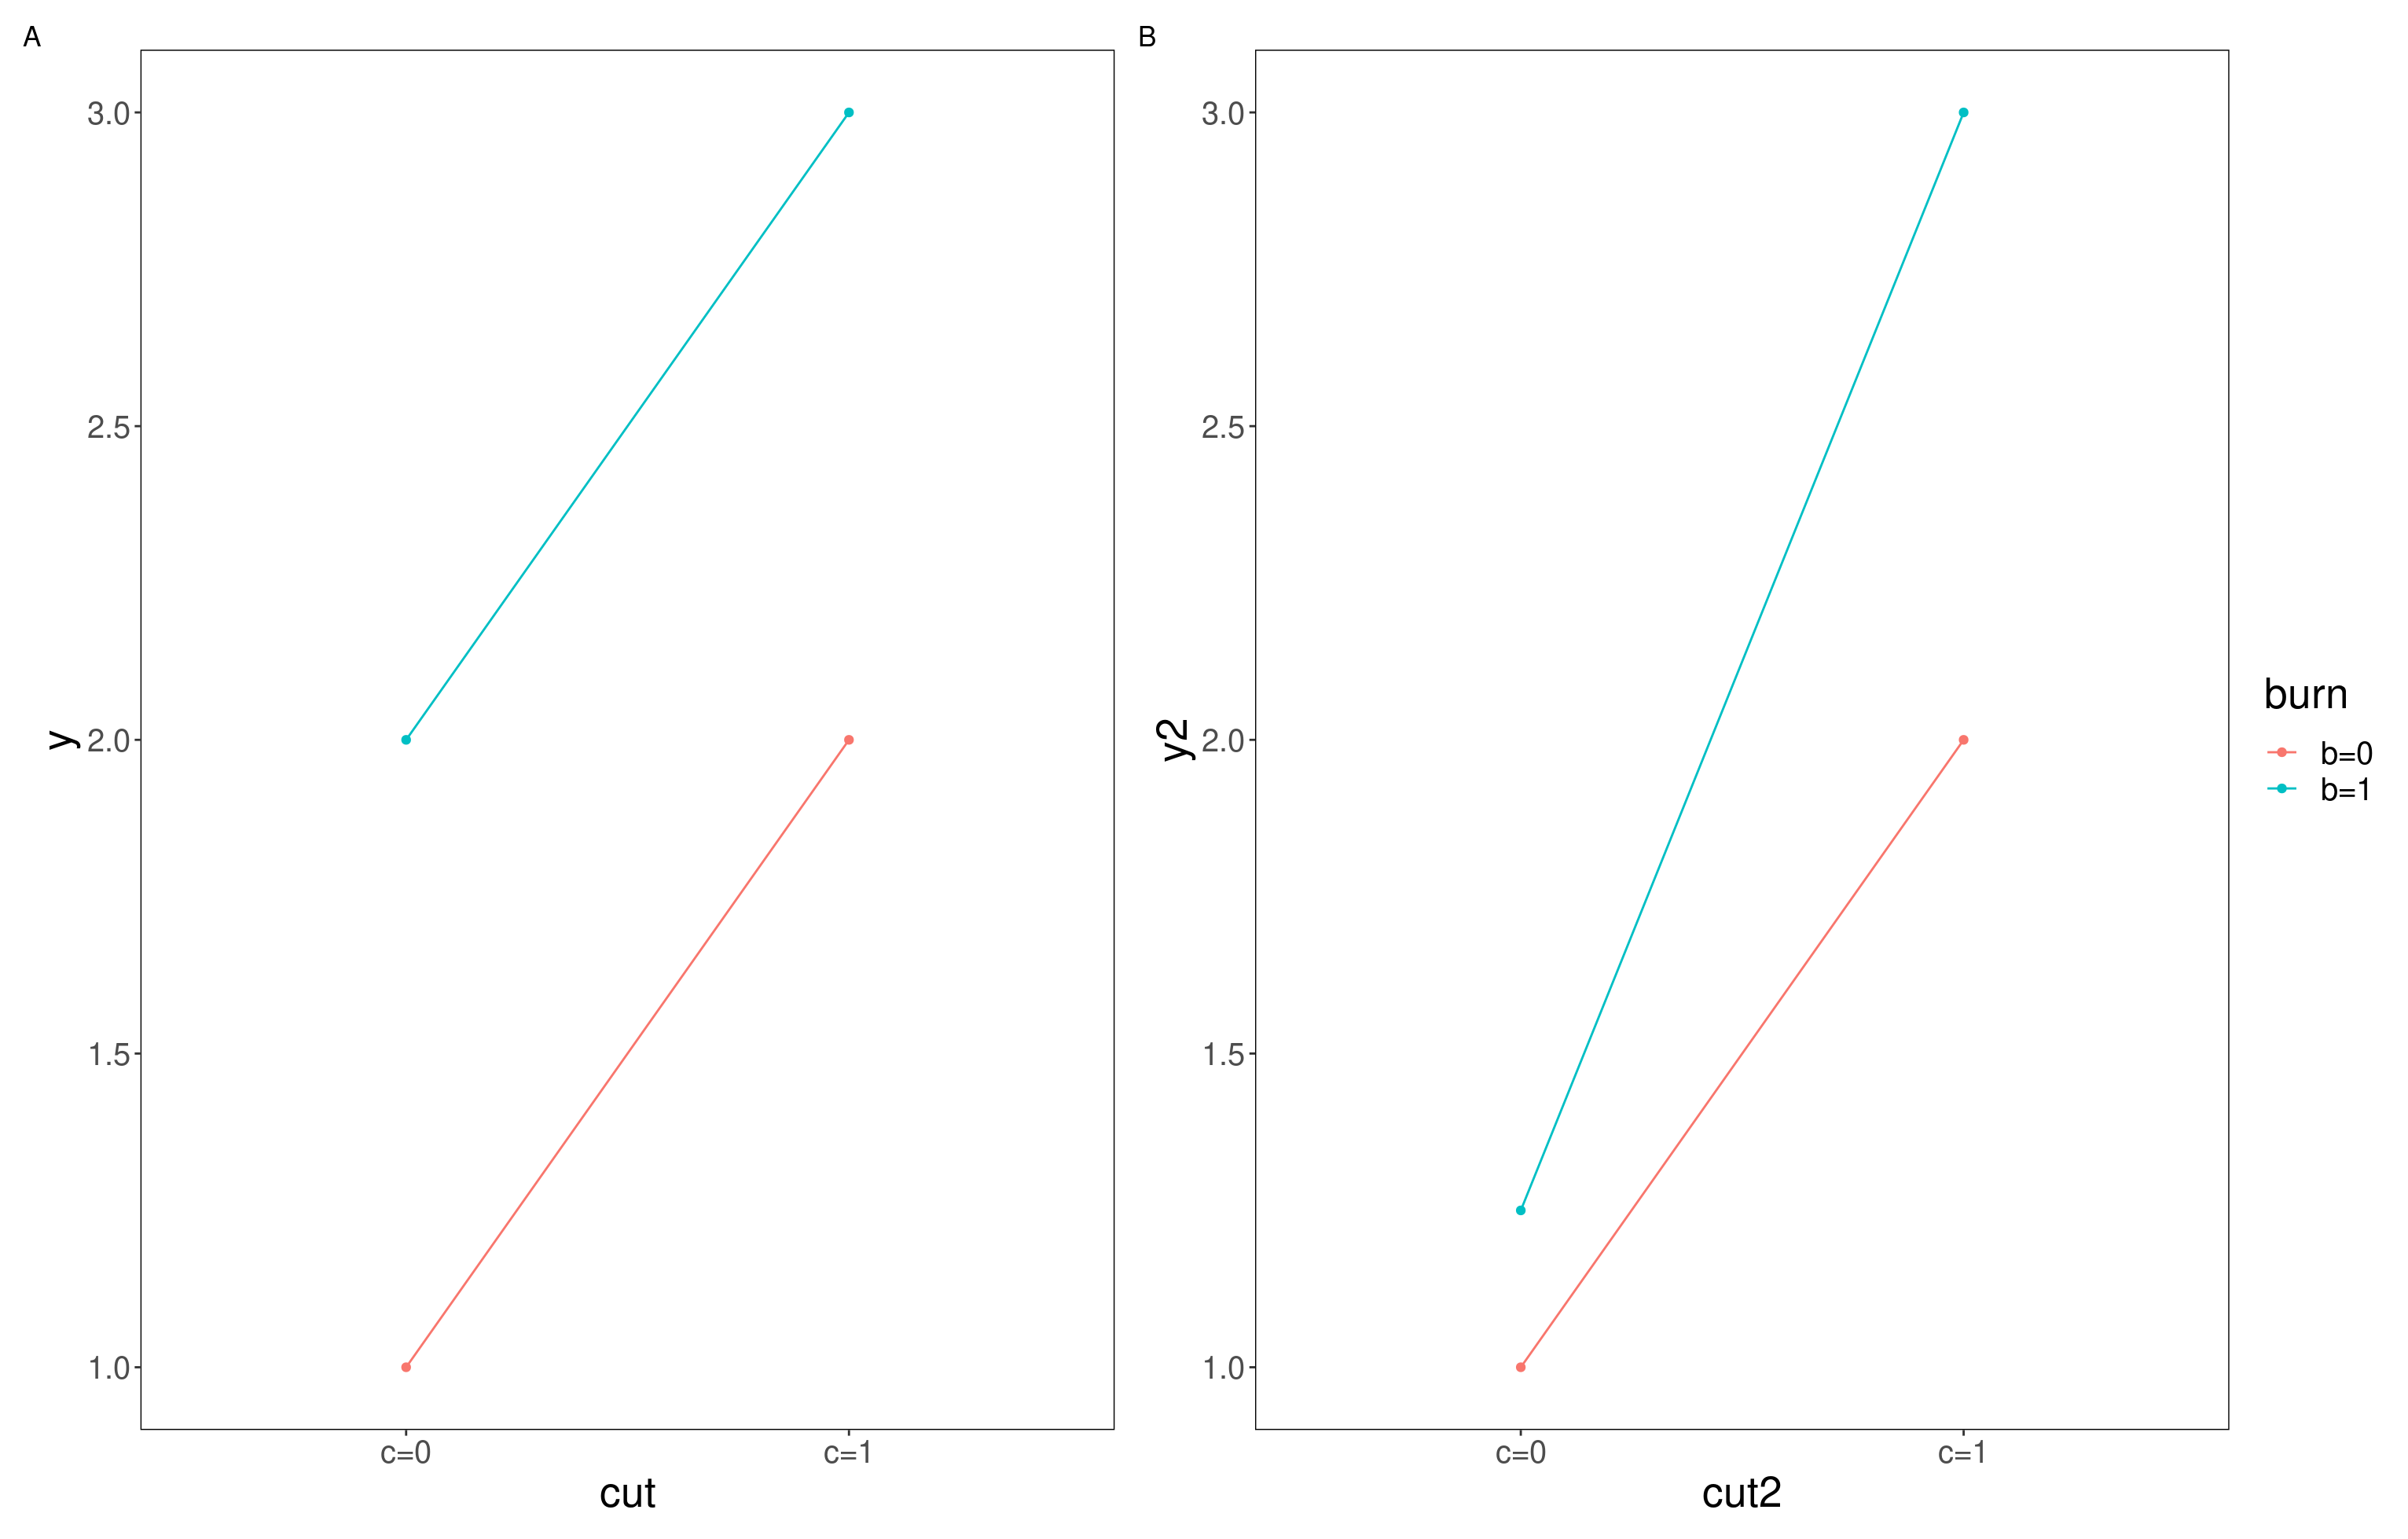
\includegraphics[width=0.9\linewidth]{figures/additive_vs_interactive} \caption{Additive vs interactive effects, A; shows an additive effect where the intercept of the two factors is different but they share a slope, B; shows an interactive effect where the interaction effect changes the relationship and so the slope also changes}\label{fig:unnamed-chunk-100}
\end{figure}

\begin{quote}
\begin{itemize}
\tightlist
\item
  Take a look at your initial box plots, do you think there is likely to be an interactive effect of the cut and burn treatments on \emph{I. cylindrica} cover in 1994?
\end{itemize}
\end{quote}

Looking at the medians here, I would guess that an interactive effect between cut and burn treatments is unlikely. But we might like to test this interpretation. This is where having our data in a factorial lay out may be helpful. Try running the following;

\begin{Shaded}
\begin{Highlighting}[]
\CommentTok{\# Construct a linear model exploring how much variation in percentage cover in the year 1994 is explained by additive and interactive effects of cut and burn treatments and additive effects of block variables}
\NormalTok{lm2 }\OtherTok{\textless{}{-}} \FunctionTok{lm}\NormalTok{(year1994 }\SpecialCharTok{\textasciitilde{}}\NormalTok{ cut }\SpecialCharTok{*}\NormalTok{burn }\SpecialCharTok{+}\NormalTok{ block, }\AttributeTok{data =}\NormalTok{ nepal)}
\FunctionTok{summary}\NormalTok{(lm2)}
\end{Highlighting}
\end{Shaded}

Remember from Chapter \ref{c12t3} we ascertained that we couldn't look for interactions with block because block isn't replicated, so here we have simply requested it be included only in an additive capacity. However we can now explore potential interactions between cut and burn treatments.

\begin{quote}
\begin{itemize}
\tightlist
\item
  What is the summary of your new model (lm2) telling you?
\end{itemize}
\end{quote}

When incorporating fixed factors with more then two levels it can also be helpful to produce the ANOVA table for your model, this will tell you the overall amount of variation explained by each factor as a whole, try running;

\begin{Shaded}
\begin{Highlighting}[]
\CommentTok{\# Produce the ANOVA table for lm2}
\FunctionTok{anova}\NormalTok{(lm2)}
\end{Highlighting}
\end{Shaded}

The variation explained by each factor is captured by the Mean sq column of this output table. The F value is then calculated by dividing the Mean sq of each line by the residual Mean sq.

\begin{quote}
\begin{itemize}
\tightlist
\item
  Are any of our factors explaining a significant part of the variation in percentact cover of \emph{I. cylindrica}?
\end{itemize}
\end{quote}

\hypertarget{exploring-the-model}{%
\subsection{Exploring the model}\label{exploring-the-model}}

Lets unpack our \texttt{lm2} model a little bit more. The \texttt{GGally} package has a super useful function called \texttt{ggcoef\_model} that produces a plot of the estimated mean difference with estimated 95\% confidence intervals. Try running the following;

\begin{Shaded}
\begin{Highlighting}[]
\CommentTok{\# Produce plots for coefficients with 95\% confidence intervals}
\FunctionTok{ggcoef\_model}\NormalTok{(lm1,}
             \AttributeTok{show\_p\_values=}\ConstantTok{FALSE}\NormalTok{,}
             \AttributeTok{signif\_stars =} \ConstantTok{FALSE}\NormalTok{,}
             \AttributeTok{conf.level=}\FloatTok{0.95}\NormalTok{)}
\end{Highlighting}
\end{Shaded}

And then run the above code again for \texttt{lm2}.

\begin{quote}
\begin{itemize}
\tightlist
\item
  Can you see the difference in how the models are structured?
\item
  What are the 95\% confidence intervals telling you here for \texttt{lm1}? Think back to our discussions in Univariate statistics around 95\% confidence intervals.
\item
  How does this compare to the plot produced for \texttt{lm2}
\end{itemize}
\end{quote}

These plots allow you to plot the estimated means and examine the interaction between treatments. Something seems to be going on with Block 3 which we may wish to investigate in more detail. We may wish to perform a Tukey test to examine these differences in more detail. To do this we will need to use the \texttt{aov()} function on our \texttt{lm()} and then perform the Tukey test on that. See below;

\begin{Shaded}
\begin{Highlighting}[]
\CommentTok{\# Run a post hoc Tukey test for lm2}
\NormalTok{lm2\_aov }\OtherTok{\textless{}{-}} \FunctionTok{aov}\NormalTok{(lm2)}
\FunctionTok{TukeyHSD}\NormalTok{(lm2\_aov, }\AttributeTok{conf.level=}\NormalTok{.}\DecValTok{95}\NormalTok{)}
\end{Highlighting}
\end{Shaded}

\begin{quote}
\begin{itemize}
\tightlist
\item
  What does the Post-Hoc Tukey test tell you about the differences between blocks?
\item
  What does your overall analysis tell you about the effects of cutting and burning in each block?
\item
  Repeat the analysis for years 1995 and 1996
\item
  Are the effects consistent across years?
\item
  Describe what the analysis shows about the effects of cutting and burning in each year.
\end{itemize}
\end{quote}

The design of a study determines the type of statistical analysis that is appropriate, and it is therefore very important to consider the type of model that you intend to use when you are designing the study.

\hypertarget{data-set-2-tulip---linear-model-with-randomised-block-designs}{%
\section{Data set 2: Tulip - Linear Model with Randomised Block designs}\label{data-set-2-tulip---linear-model-with-randomised-block-designs}}

Lets look at another data set; \texttt{tulip.csv}. These data are from a study of the effects of different levels of shade and irrigation on the production of tulip flowers. There are three shade treatments and three water level treatments, giving a total of nine combinations. The entire experiment was replicated over three different flower beds.

The datafile therefore contains the following variables:

\begin{itemize}
\tightlist
\item
  bed: flower bed 1, 2 or 3
\item
  water: water levels 1, 2 or 3
\item
  shade: shade levels 1, 2 or 3
\item
  blooms: number of tulip blooms produced per plant
\end{itemize}

\hypertarget{task-5---checking-the-data}{%
\subsection{Task 5 - Checking the data}\label{task-5---checking-the-data}}

Load the dataset \texttt{tulip.csv} into your workspace under the object name \texttt{tulip} and try performing some routine checks to make sure R has interpreted the variables correctly and that all expected data is present and accounted for. You can use some of the functions explored in Chapter \ref{checking-the-data} if you need some help with this.

\begin{quote}
Look at each of your variables, are any of them categorical? Has R characterised them as double (\texttt{dbl}), character (\texttt{chr}) or factor (\texttt{fct}) variables?
Do some of these need to be changed? Remember you can use the \texttt{as.factor()} function to alter these (see Chapter \ref{c11t1}).
\end{quote}

\hypertarget{task-6---exploring-the-data}{%
\subsection{Task 6 - Exploring the data}\label{task-6---exploring-the-data}}

You are going to need to construct a linear model to explore how tulip flower production varies among the shade and water treatments. But first it may be helpful to visualise our data using box\_plots. See if you can construct a box plot with \texttt{water} treatment on the x axis, \texttt{blooms} on the y axis and coloured by the \texttt{shade} treatment.

\begin{quote}
\begin{itemize}
\tightlist
\item
  What do you notice about this plot?
\item
  Do you notice any possible additive or interactive effects?
\end{itemize}
\end{quote}

Before we start modeling, we need to check that our data meets the assumptions of the linear model. Start by calculating some descriptive statistics for each treatment and consider what you think the effects of the predictor variables and whether the data meet the assumptions of the linear model. Build some histograms and run Levenes Test to check the assumptions of the linear model -- normality of the data for each treatment and equality of variance between treatments.

\hypertarget{playing-with-some-models}{%
\subsection{Playing with some models}\label{playing-with-some-models}}

Construct the linear model with \texttt{bloom} as the dependent variable and \texttt{bed}, \texttt{water} and \texttt{shade} as fixed factors. As with the Nepal data, you have a randomized block experiment here, as the water and shade treatments are replicated across three flower beds (blocks). You therefore have to customize the model with an interactive term between \texttt{water} and \texttt{shade} and an additive term for \texttt{bed} (remember, this is to avoid the model trying to look for interactions with \texttt{bed}).

\begin{quote}
\begin{itemize}
\tightlist
\item
  Run the model and write down what the model output tells you about the effect of each treatment and the effects of the interaction between treatments on tulip production. You may find it helpful to use both \texttt{summary()} and \texttt{anova()} functions.\\
\item
  Look back at your original boxplot, does your analysis corroborate the plot?
\item
  What is the effect of the treatments on tulip production
\end{itemize}
\end{quote}

The interaction term of water:shade is significant (p = 0.005). You can see why most easily by looking at our original box plot. At shade 1, there are big differences among the water treatments while, at shade levels 2 \& 3, there is only a slight increase in blooms at water level 3. Shade 1 is the lowest shade level, and water 3 is the highest water level, so this suggests that watering more is most helpful when there is little shade, an interpretation supported by the low bloom response at water level 1 and shade level 1.

The effect of water therefore depends on shade level. Tulip bloom production increases strongly with increasing water levels at low shade 1, but less so at higher shades. However, overall there seems to be an overall positive effect on blooms going from 1 to 3 for any given shade level.

\hypertarget{mixed-effects-linear-models}{%
\section{Mixed effects linear models}\label{mixed-effects-linear-models}}

In some cases, you may wish to include model predictors that may have an influence on your dependent variable but for which you only want to account for that effect, i.e.~not measure it directly -- these are known as \textbf{random} factors. For example, in both the Nepal and Tulip examples, the data were grouped together in space (\textbf{block} in Nepal and \textbf{bed} in Tulip). As an alternative to a customised model design, we could have included this grouping predictor as a random factor.

If you are including random and fixed effects in one model we are constructing something called a mixed effects model, and random effects must have more than two levels (but ideally these models work best if you have at least 5 levels).

We will see if how this works now, with our \texttt{tulip.csv} data set.

Previously, we constructed a customised linear model to analyse these data but an alternative would be to construct a mixed model and account for the non-independence of plants from the same flowerbed by including \texttt{bed} as a random factor. This will mean that the model accounts for the variation that can be attributed to bed but will not statistically compare the three flowerbeds.

To construct a mixed effects model we will be making use of the function \texttt{lmer} from the \texttt{lmerTest} package. Try running the following;

\begin{Shaded}
\begin{Highlighting}[]
\CommentTok{\# Run a mixed effects linear model}
\NormalTok{mixed\_model }\OtherTok{\textless{}{-}} \FunctionTok{lmer}\NormalTok{(blooms }\SpecialCharTok{\textasciitilde{}}\NormalTok{ water}\SpecialCharTok{*}\NormalTok{shade }\SpecialCharTok{+}\NormalTok{ (}\DecValTok{1}\SpecialCharTok{|}\NormalTok{bed), }\AttributeTok{data =}\NormalTok{ tulip)}
\end{Highlighting}
\end{Shaded}

And then check out the output by using \texttt{summary()} and \texttt{anova()} functions.

\begin{quote}
\begin{itemize}
\tightlist
\item
  What does these functions tell you about the effects of water and shade on the numbers of blooms produced?
\item
  Compare the F values in the ANOVA output to those that you found when you constructed a customised linear model \texttt{tulip}.
\end{itemize}
\end{quote}

You might have noticed that the \texttt{summary()} output for your mixed effects model is very similar to that of your standard linear model. And this is broadly true. The additional section to pay attention to is the \texttt{Random\ effects:} table, this gives you additional information on how much of the variation from your mixed effects model is explained by your random factor (in this case bed).

The results of these two modelling approaches are, in this case, the same and either of these models would be an appropriate way to analyse these data. In this case, including bed as a fixed or random effect makes little difference to the model but if there had been many different beds and a less balanced design, it is likely that the mixed model would be more powerful (as fitting \texttt{bed} as a random effect leaves more degrees of freedom for the model, and thus there is more power to find any effects that exist).

\hypertarget{conclusions}{%
\section{Conclusions}\label{conclusions}}

Today we have explored how the way you conduct a study influences how you structure your model. We have examined the differences between additive and interactive effects and how to spot the hallmarks of each and we have dabbled with incorporating random effects into a mixed effects linear model.

These sessions are very much introductions into the world of multivariate statistics and your knowledge will benefit from further reading. I highly recommend Getting Started with R; An Introduction for Biologists by Beckerman, Childs and Petchey for further reading.

\hypertarget{before-you-leave-9}{%
\section{Before you leave!}\label{before-you-leave-9}}

Make sure you save your script and download it if you would like to keep a local copy.

Please log out of posit Cloud!

\hypertarget{repeated-measures-linear-models}{%
\chapter{Repeated Measures Linear Models}\label{repeated-measures-linear-models}}

This chapter will run in Workshop 9 of Week 9.

\hypertarget{introduction-7}{%
\section{Introduction}\label{introduction-7}}

When we are exploring the effect of different treatments on a dependent variable, the most powerful method is to include the same individuals within each treatment. This method allows you to explore the effect of the treatment, having controlled for the inherent variation among individuals in their response to the treatments. This is called a Repeated Measures design. For example, if you were measuring how the growth of plants changed over time with the addition of a nutrient, you could either measure different plants from each treatment (nutrient versus control) at each time interval (e.g.~every week), or you could measure the same plants at each time interval -- the latter is much more powerful because individual variation in plant growth (independent of the treatment) can be controlled in the analysis.

\hypertarget{practical-9---repeated-measures-linear-models}{%
\section{Practical 9 - Repeated Measures Linear Models}\label{practical-9---repeated-measures-linear-models}}

In this session we will be working with two data sets. First of all we have \texttt{activity.csv} which measures sweat produced in 10 individuals during a bout of intense activity. We will then move onto \texttt{metabolism.csv} which measures metabolism in a migrant bird species under different conditions, so we will look at how we can implement repeated measures design in a two-way ANOVA.

Log into the Posit cloud classroom and install and load the following packages; \texttt{tidyverse}and \texttt{rstatix}.

\hypertarget{data-set-1---activity}{%
\section{Data set 1 - Activity}\label{data-set-1---activity}}

This is an example of where repeated measured design was used to measure sweat produced in 10 individuals at three time points before, during and after a bout of intense physical activity.

\begin{itemize}
\tightlist
\item
  \texttt{activity.csv} data file
\end{itemize}

This data file contains the following data;

\begin{itemize}
\tightlist
\item
  time0 - amount of sweat produced before activity
\item
  time1 - amount of sweat produced during activity
\item
  time2 - amount of sweat produced after activity
\end{itemize}

\hypertarget{task-1---checking-the-data-3}{%
\subsection{Task 1 - Checking the data}\label{task-1---checking-the-data-3}}

Load the data set \texttt{activity.csv} into your workspace under the object name \texttt{activity} and try performing some routine checks to make sure R has interpreted the variables correctly and all expected data is present and accounted for. You can use some of the functions explored in Chapter \ref{checking-the-data} if you need some help with this.

We are going to have to do some data wrangling before we can continue this analysis. We really need an individual identifier here so we can relate individual participants back to their scores at each time point. Try running the following;

\begin{Shaded}
\begin{Highlighting}[]
\CommentTok{\# Create an object with individual identifiers (1 to 10)}
\NormalTok{individual }\OtherTok{\textless{}{-}} \FunctionTok{c}\NormalTok{(}\DecValTok{1}\SpecialCharTok{:}\DecValTok{10}\NormalTok{)}
\CommentTok{\# Bind our \textasciigrave{}individual\textasciigrave{} object as a column to our \textasciigrave{}activity\textasciigrave{} data frame}
\NormalTok{activity }\OtherTok{\textless{}{-}} \FunctionTok{cbind}\NormalTok{(activity,individual)}
\end{Highlighting}
\end{Shaded}

\begin{quote}
\begin{itemize}
\tightlist
\item
  Make sure you understand how the above piece of code works.
\item
  Is our data frame in a wide or a long format? Which format do you think it should be in?
\end{itemize}
\end{quote}

Make sure your data is in a long format, try running the following to put your time columns into a long format;

\begin{Shaded}
\begin{Highlighting}[]
\NormalTok{activity }\OtherTok{\textless{}{-}}\NormalTok{ activity }\SpecialCharTok{\%\textgreater{}\%}
  \FunctionTok{pivot\_longer}\NormalTok{(}\AttributeTok{cols =}\NormalTok{ time0}\SpecialCharTok{:}\NormalTok{time2,}
               \AttributeTok{names\_to =} \StringTok{"time\_point"}\NormalTok{, }
               \AttributeTok{values\_to =} \StringTok{"response"}\NormalTok{)}
\end{Highlighting}
\end{Shaded}

\begin{quote}
\begin{itemize}
\tightlist
\item
  Now use \texttt{glimpse()} to check how R has categorised the different data types for each variable?
\item
  Really we need \texttt{individual} and \texttt{time\_point} to be categorised as factors. See if you can use \texttt{as.factor()} to convert these variables to factors.
\end{itemize}
\end{quote}

\hypertarget{task-2---exploring-the-data-2}{%
\subsection{Task 2 - Exploring the data}\label{task-2---exploring-the-data-2}}

Now that we have our data in a sensible format we can start to do some data exploration.

\begin{quote}
\begin{itemize}
\tightlist
\item
  Start by calculating the means and SE for each of the three time periods.
\item
  Write down what this tells you about the effect of activity on sweat production.
\item
  Do you think that these groups are likely to differ significantly from one another?
\end{itemize}
\end{quote}

Lets try to make a data visualisation to help with this last point

\begin{quote}
\begin{itemize}
\tightlist
\item
  See if you can make a boxplot with \texttt{time\_point} on the x axis and \texttt{response} on the y axis.
\item
  Draw histograms to check the assumption of normally distributed data.
\item
  Is this assumption met for all three groups?
\end{itemize}
\end{quote}

\hypertarget{task-3---playing-with-some-statistics}{%
\subsection{Task 3 - Playing with some statistics}\label{task-3---playing-with-some-statistics}}

You could explore the difference between the sweating rates of individuals before, during or after activity by running a one-way ANOVA (i.e.~a linear model with sweat production as the dependent variable and the three time periods as predictors). However, as the same 10 people took part in all three treatments, a more powerful analysis is a Repeated Measures ANOVA\ldots{}

To run this model we are going to start using a new ANOVA function. Here we need to define a subject identifier, within subject factor (or grouping variable) and our dependent variable. Try running the following;

\begin{Shaded}
\begin{Highlighting}[]
\CommentTok{\# Run a repeated measures ANOVA comparing response (dependent variable) between different time points (within subject variable) across individuals (subject identifier)}
\NormalTok{repeated\_aov }\OtherTok{\textless{}{-}} \FunctionTok{anova\_test}\NormalTok{(}\AttributeTok{data =}\NormalTok{ activity, }\AttributeTok{dv =}\NormalTok{ response, }\AttributeTok{wid =}\NormalTok{ individual, }\AttributeTok{within =}\NormalTok{ time\_point)}
\CommentTok{\# Call the ANOVA table for our model}
\FunctionTok{get\_anova\_table}\NormalTok{(repeated\_aov)}
\end{Highlighting}
\end{Shaded}

You will be aware that ANOVAs make a range of assumtions of the input data. The repeated measures ANOVA has an additional assumption - sphericity. Sphericity is a test of the assumption of equality of variance among treatments. Generally a Mauchley's test is applied to test for this and if p \textgreater{} 0.05, then there is no significant differences between the variances of the treatments, and the assumption is met. If p \textless{} 0.05, then the variances between your treatments are significantly different and the test assumption is violated.

Very conveniently, get\_anova\_table() does a lot of the work for you. It automatically checks the sphericity assumption using Mauchley's test and if the sphericity assumption is violated then it will automatically apply a correction (the Greenhouse\_Geisser sphericity correction) to within subject factors that are in violation of the sphericity assumption. Applying the correction essentially reduces the degrees of freedom to make the test more conservative.

Take a look at the output from the \texttt{get\_anova\_table()} function. This output is a little different from other ANOVA outputs we've seen so far. DFn and DFd represent the degrees of freedom for treatment (T-1) and error ((T-1)(n-1)) respectively. The F statistic, represents the ratio of the variance between groups to the variance within groups and the p value which gives the probability of seeing the test statistic if the null hypothesis were true. Finally the \texttt{ges} gives a general effect size, i.e.~the amount of variability due to the within subject factor.

\begin{quote}
\begin{itemize}
\tightlist
\item
  Write down a few lines interpreting the output of this analysis
\item
  Does this match what you might think from the boxplot?
\end{itemize}
\end{quote}

A post-hoc test would be helpful here to add some direction to the differences we are seeing. With repeated measures ANOVA, Bonferroni post-hoc test is the recommended test. We can perform this using the following piece of code;

\begin{Shaded}
\begin{Highlighting}[]
\NormalTok{pwc }\OtherTok{\textless{}{-}}\NormalTok{ activity }\SpecialCharTok{\%\textgreater{}\%}
  \FunctionTok{pairwise\_t\_test}\NormalTok{(}
\NormalTok{    response }\SpecialCharTok{\textasciitilde{}}\NormalTok{ time\_point, }\AttributeTok{paired =} \ConstantTok{TRUE}\NormalTok{,}
    \AttributeTok{p.adjust.method =} \StringTok{"bonferroni"}
\NormalTok{  )}
\NormalTok{pwc}
\end{Highlighting}
\end{Shaded}

\begin{quote}
\begin{itemize}
\tightlist
\item
  Take a look at the output, how would you interpret this?
\item
  What does this output tell you about the differences among treatments?
\end{itemize}
\end{quote}

So we have played with some very basic repeated measures analysis, essentially a one-way repeated measures ANOVA. But often if you are using repeated measures designs you will want to incorporate more variables.

\hypertarget{data-set-2---metabolism}{%
\section{Data set 2 - Metabolism}\label{data-set-2---metabolism}}

Now we can start to play with a slightly more complex data set and analysis.

We will look at a study of the metabolism of migrant birds under different environmental (temperature) and physiological (parasite load) conditions. The metabolism of 30 different birds was measured at three different time periods (1 = after 10 minutes, 2 = after two hours, 3 = after four hours), under either warm (inside) or cold (outside) temperatures, and the parasite load of each bird (low, medium, high) was measured at the end of the experiment. The data for this can be found in;

\texttt{bird\_metabolism.csv}

The data in this file is as follows;

\begin{itemize}
\tightlist
\item
  individual - individual identifier
\item
  para - an index or parasite load (1 = low parasite load, 2 = medium parasite load and 3 = high parasite load)
\item
  temp - temperature conditions (1 = warm, 2 = cold)
\item
  met1 - metabolism at time point 1 (after 10 minutes)
\item
  met2 - metabolism at time point 2 (after two hours)
\item
  met3 - metabolism at time point 3 (after four hours)
\end{itemize}

\hypertarget{task-4---checking-the-data}{%
\subsection{Task 4 - Checking the data}\label{task-4---checking-the-data}}

Load the data set \texttt{metabolism.csv} into your workspace under the object name \texttt{metabolism} and try performing some routine checks to make sure R has interpreted the variables correctly and all expected data is present and accounted for. You can use some of the functions explored in Chapter \ref{checking-the-data} if you need some help with this.

\begin{quote}
\begin{itemize}
\tightlist
\item
  Which variables are you going to include as fixed factors. Has R interpreted these variables as factors?
\item
  Is this data set in a wide or a long format? Does it need to be converted?
\end{itemize}
\end{quote}

Both \texttt{temp} and \texttt{para} are categorical and need to be identified as factors and the columns \texttt{met1}, \texttt{met2}, \texttt{met3} need to be in a single column. Have a go at creating some code to complete both of these tasks. Look at earlier sections if you get stuck.

\hypertarget{task-5---exploring-the-data}{%
\subsection{Task 5 - Exploring the data}\label{task-5---exploring-the-data}}

Now that we have our data in a sensible format we can start to do some data exploration.

\begin{quote}
\begin{itemize}
\tightlist
\item
  Start by calculating the means and SE for each of the different time points
\end{itemize}
\end{quote}

Lets try to make some data visualisation to help explore this data set.

\begin{quote}
\begin{itemize}
\tightlist
\item
  See if you can make a boxplot with time point on the x axis and metabolism on the y axis. Colour your boxes by \texttt{temp}
\item
  Now create another boxplot but try colouring the boxes by \texttt{para}
\item
  What do these box plots tell you about the effects of time, temperature and parasites on metabolism?
\item
  Draw histograms to check the assumption of normally distributed data.
\item
  Is this assumption met for all time points?
\end{itemize}
\end{quote}

\hypertarget{task-6---playing-with-some-statistics}{%
\subsection{Task 6 - Playing with some statistics}\label{task-6---playing-with-some-statistics}}

Now we are ready to start playing with some statistics.

\begin{Shaded}
\begin{Highlighting}[]
\CommentTok{\# Fun a repeated measures ANOVA with metabolism as the dependent variable, individul as the subject identifier, time as the within subject variable and temp and para as between subject variables.}
\NormalTok{met\_aov }\OtherTok{\textless{}{-}} \FunctionTok{anova\_test}\NormalTok{(}
  \AttributeTok{data =}\NormalTok{ metabolism, }\AttributeTok{dv =}\NormalTok{ metabolism, }\AttributeTok{wid =}\NormalTok{ individual,}
  \AttributeTok{within =}\NormalTok{  time, }\AttributeTok{between =} \FunctionTok{c}\NormalTok{(temp,para))}
\FunctionTok{get\_anova\_table}\NormalTok{(met\_aov)}
\end{Highlighting}
\end{Shaded}

\begin{quote}
\begin{itemize}
\tightlist
\item
  What does the output tell you about the variation in metabolism over the three time periods?
\item
  What do the interactions with time rows tell you?
\item
  What do the tests between subject variables tell you about the effects of parasite load and temperature on metabolism?
\item
  Run a post-hoc test to get more information on the direction of some of these relationships.
\item
  How do your conclusions here compare to the conclusions you drew from the box plots earlier?
\end{itemize}
\end{quote}

\hypertarget{conclusions-1}{%
\section{Conclusions}\label{conclusions-1}}

This session we have explored how we can incorporate repeated measures designs into our analysis by using repeated measures ANOVAs.

\hypertarget{before-you-leave-10}{%
\section{Before you leave!}\label{before-you-leave-10}}

Make sure you save your script and download it if you would like to keep a local copy.

Please log out of posit Cloud!

\hypertarget{a-very-introductory-introduction-to-generalised-linear-models}{%
\chapter{A Very Introductory Introduction to Generalised Linear Models}\label{a-very-introductory-introduction-to-generalised-linear-models}}

This chapter will run in Workshops 10 and 11 of Week 10.

\hypertarget{introduction-8}{%
\section{Introduction}\label{introduction-8}}

This week we will start to explore the world of generalised linear models (GLMs), not to be confused with general linear models (that have underpinned all of the statistical techniques we have studies so far).

\hypertarget{what-is-a-generalised-linear-model-and-why-are-they-useful}{%
\subsection{What is a Generalised Linear Model and why are they useful?}\label{what-is-a-generalised-linear-model-and-why-are-they-useful}}

We have so far spent a lot of time thinking about the general linear model family (including regressions, ANOVAs and ANCOVAs). We have also spent some time dealing with assumptions. All of these models make certain assumptions about the data they are dealing with and some of these assumptions are held in common within the general linear model family.

Of the dependent/response variable they all assume;

\begin{itemize}
\tightlist
\item
  A continuous variable that can have both positive and negative values as well as fractions
\item
  That the data are unbounded (although this is somewhat loosely applied, size, for example, cannot be negative)
\item
  Equal variance\\
\item
  A normal distribution
\end{itemize}

You will have checked the distribution and equality of variance for all of our previous analyses and where these assumptions were violated we either transformed the data or performed non-parametric alternative tests.

However often in the biological sciences you will be collecting data that is not appropriate for use in general linear models. For example your response variable may be count data (so bounded, counts cannot go below 0) or binary (e.g.~presence/absence, denoted by 1s and 0s), or another type of categorical data. Here a general linear model would be inappropriate and this is where GLMs really come into their own.

These workshops will be, in no way, a definitive guide to the minutia of GLMs, but we will cover a couple of common usages and have a think about what you need to look out for to ensure your model is an appropriate fit for your data. If you use this family of models on your own data (which, if you continue in the field of ecology, you almost certainly will) you will need to do additional reading and also, probably, spend quite a lot of time playing with different model structures to become proficient.

\hypertarget{key-parts-of-a-glm}{%
\subsection{Key parts of a GLM}\label{key-parts-of-a-glm}}

The implementation of GLMs in R is quite different to the other models we have previously constructed. There are three additional components to be aware of;

\begin{itemize}
\tightlist
\item
  \textbf{Linear Predictor} - this sounds scarier then it is. You have all already used linear predictors. This is an equation which describes how the predictor variables affect the response variable. With our linear models an example of this was;
\end{itemize}

\[
y = mx + c
\]

\begin{itemize}
\tightlist
\item
  \textbf{Family} - also known as the error structure. This is the probability distribution that describes the response variable and that will underpin how your GLM treats your data.
\item
  \textbf{Link Function} - this accompanies your family argument and provides a link between the linear predictor and the probability distribution.
\end{itemize}

\hypertarget{different-famlies-and-their-link-functions}{%
\subsection{Different famlies and their link functions}\label{different-famlies-and-their-link-functions}}

The family (or error structure) you select for your GLM will depend on how your data look, but the most common ones are listed below.

\begin{longtable}[]{@{}
  >{\centering\arraybackslash}p{(\columnwidth - 10\tabcolsep) * \real{0.1667}}
  >{\centering\arraybackslash}p{(\columnwidth - 10\tabcolsep) * \real{0.1667}}
  >{\centering\arraybackslash}p{(\columnwidth - 10\tabcolsep) * \real{0.1667}}
  >{\centering\arraybackslash}p{(\columnwidth - 10\tabcolsep) * \real{0.1667}}
  >{\centering\arraybackslash}p{(\columnwidth - 10\tabcolsep) * \real{0.1667}}
  >{\centering\arraybackslash}p{(\columnwidth - 10\tabcolsep) * \real{0.1667}}@{}}
\toprule\noalign{}
\begin{minipage}[b]{\linewidth}\centering
Data Distribution
\end{minipage} & \begin{minipage}[b]{\linewidth}\centering
Family
\end{minipage} & \begin{minipage}[b]{\linewidth}\centering
Default Link Function
\end{minipage} & \begin{minipage}[b]{\linewidth}\centering
Link Function
\end{minipage} & \begin{minipage}[b]{\linewidth}\centering
R code
\end{minipage} & \begin{minipage}[b]{\linewidth}\centering
\end{minipage} \\
\midrule\noalign{}
\endhead
\bottomrule\noalign{}
\endlastfoot
Normal & Gaussian & Identity & \(gμ = μ\) & \texttt{gausian(link="identity")} & \\
Poisson & Poisson & Log & \(g(μ) = log(μ)\) & \texttt{poisson(link="log")} & \\
Binomial & Binomial & Logit & \(g(μ)= log(\frac{μ}{1-μ})\) & \texttt{binomial(link="logit")} & \\
Gamma & Gamma & Inverse & \(g(μ)= \frac{1}{μ}\) & \texttt{gamma(link="inverse")} & \\
\end{longtable}

These are just a few of the more commonly used GLM error structures and their default link functions that you are likely to come across. We will explore two of these in more depth over the course of this week.

\hypertarget{glms-with-a-poisson-error-structure}{%
\subsection{GLMs with a Poisson Error Structure}\label{glms-with-a-poisson-error-structure}}

As ecologists you will frequently find that the data you are collecting is count data. Count data is inherently tricky to analyse using general linear model approaches. For a start it breaks the assumption that the data are unbounded (it cant go below 0) and often it cannot form fractions (often we count in whole numbers only), so really its discrete data. These two factors mean that count data are unlikely to conform to a normal distribution, which works with continuous data and allows for negative values (neither of which are permitted by count data). In addition, normal distributions are symetrical, with half of the data points falling on either side of the mean. Count data (often but not always) has a greater number of data points towards the lower end of the x axis. So it will be positively skewed and follow a Poisson distribution.

If we come across data like this, we could try doing some log transformations and that might fix the issue or it might not. Or if we only want to build a simple model we could explore non-parametric alternatives to our general linear models. But sometimes we want to build a more complex model with several independent variables and sometimes log transformations just don't cut it anymore. So here we may consider performing a GLM with a poisson error structure and log link function.

So our model would look something like this;

\[
y = log_e^{mx+c}
\]

\hypertarget{glms-with-a-binomial-error-structure}{%
\subsection{GLMs with a Binomial Error Structure}\label{glms-with-a-binomial-error-structure}}

You may also end up designing your experiment in such a way that your response/dependent variable is categorical and/or binary. For example, commonly ecologists use binary data to measure the presence or absence of a species. When we have a categorical or binary response variable we will automatically be breaking several of the assumptions of the general linear models (i.e.~the response is not continuous, it is bounded and it wont conform to a normal distribution). This is where GLMs with a binomial error structure come in super handy (they essentially perform something akin to a logistic regression, you may see these refereed to in the literature).

When we construct a model with a binary (or categorical) dependent variable, such as presence or absence, we are essentially asking which independent variables make it more or less probable that we will detect the presence of a species. This can be expressed mathematically like this;

\[
P(Y) = \frac{e^z}{(1+e^z)}
\]

Where \(P(Y)\) is the probability of a given Y value (e.g.~present or absent), \(e\) is the base of natural logarithms and \(z\) is the linear regression equation (\(m_1x_1+m_2x_2+m_3x_3+...c\)). The above equation can then be rearranged to;

\[
log_e(\frac{P(Y)}{1-P(Y)}) = m_1x_1 + m_2x_2+m_3x_3 +... c
\]
So, this equation is the (natural logarithm of) the probability of being in one group (e.g.~present) divided by the probability of being in the other group (e.g.~absent). The predictor coefficients (slope (m) and intercept (c)) are used in the same way as in regression, but instead of predicting an actual value of Y, they predict the probability of Y being in one group or the other. Neat right???

\hypertarget{practical-10---glms}{%
\section{Practical 10 - GLMs}\label{practical-10---glms}}

This week we will be working through three data sets;

\begin{itemize}
\tightlist
\item
  Sheep
\item
  Frogs
\item
  The return of the Kooki bird
\end{itemize}

I have created a new Classroom in Posit cloud for you to work from this week. Follow the link \href{https://posit.cloud/spaces/451048/join?access_code=SiQlhHzulmeBkbO4NcMfueUek8iqroLUiJnPLxJU}{here}. Please note, to hopefully fix the issues around crashes last week, I have installed all of the packages in advance, you can see this in the script called \texttt{startup.R} saved in the workspace. The package installations are hashed out, you will still need to load \texttt{tidyverse}, \texttt{performance}, \texttt{pscl}, \texttt{lme4}, \texttt{Matrix} and \texttt{MASS} with the \texttt{library()} function but you WONT need to run \texttt{install.packages()} at all.

\hypertarget{a-poisson-glm-on-some-beautifully-behaved-data}{%
\section{A Poisson GLM on some beautifully behaved data}\label{a-poisson-glm-on-some-beautifully-behaved-data}}

Our first workshop mirrors an excellent workshop taken from Beckerman et al., 2017. The data were collected from the Soay sheep population on the island of Hirta (Scotland). Scientists wanted to know if lifetime reproductive success (number of live young produced over the course of a lifetime) increased with the average body mass of female sheep (ewes). This data set is very neat, quite simple and beautifully well behaved so makes for a great starting point with your first GLM. I also highly recommend this publication if you wish for further reading.

\begin{itemize}
\tightlist
\item
  \texttt{SoaySheepFitness.csv} data file
\end{itemize}

This data file contains the following data;

\begin{itemize}
\tightlist
\item
  fitness - the number of offspring produced over a ewes lifetime
\item
  body.size - the average body mass of each ewe
\end{itemize}

\hypertarget{task-1---check-the-data}{%
\subsection{Task 1 - Check the data}\label{task-1---check-the-data}}

Load the data set \texttt{SoaySheepFitness.csv} into your workspace under the object name \texttt{sheep} and try performing some routine checks to make sure R has interpreted the variables correctly and all expected data is present and accounted for. You can use some of the functions explored in Chapter \ref{checking-the-data} if you need some help with this.

\hypertarget{task-2---exploring-the-data-3}{%
\subsection{Task 2 - Exploring the data}\label{task-2---exploring-the-data-3}}

As always, its a really good idea to explore your data set before you start launching into more advanced analyses.

\begin{quote}
\begin{itemize}
\tightlist
\item
  Build a histogram for \texttt{fitness} what does the distribution of the data look like?
\item
  Is a mean going to be a fair reflection for this data distribution?
\item
  Build a scatter plot with \texttt{body.size} on the x axis and \texttt{fitness} on the y axis, how would you interpret this plot, what shape is it?
\end{itemize}
\end{quote}

Try adding the following line to the code for your scatter plot;

\begin{Shaded}
\begin{Highlighting}[]
\FunctionTok{geom\_smooth}\NormalTok{(}\AttributeTok{method =} \StringTok{"lm"}\NormalTok{, }\AttributeTok{se =} \ConstantTok{FALSE}\NormalTok{)}
\end{Highlighting}
\end{Shaded}

\begin{quote}
\begin{itemize}
\tightlist
\item
  Does this regression line fairly reflect the data?
\end{itemize}
\end{quote}

Spoilers, no not really, a curve would be a much better fit for these data. Try adding this additional line to your scatter plot code;

\begin{Shaded}
\begin{Highlighting}[]
\FunctionTok{geom\_smooth}\NormalTok{(}\AttributeTok{span =} \DecValTok{1}\NormalTok{, }\AttributeTok{colour =} \StringTok{"red"}\NormalTok{, }\AttributeTok{se =} \ConstantTok{FALSE}\NormalTok{)}
\end{Highlighting}
\end{Shaded}

\begin{quote}
\begin{itemize}
\tightlist
\item
  Hopefully you have two lines on your scatter plot, which one is a better fit, blue or red?
\end{itemize}
\end{quote}

These kinds of patterns are classic for poisson distributions. We could try and build a linear model with these data and R would let you, but the model fit would be terrible and you would run the risk of producing a nonsensical analysis.

Instead lets try fitting a generalised linear model with a poisson error structure.

\hypertarget{task-3---fitting-a-glm}{%
\subsection{Task 3 - Fitting a GLM}\label{task-3---fitting-a-glm}}

So our first GLM. There is a nice simple function for fitting this model, try running the following;

\begin{Shaded}
\begin{Highlighting}[]
\CommentTok{\# Running a GLM with poisson error structure and log link function}
\NormalTok{sheep\_glm }\OtherTok{\textless{}{-}} \FunctionTok{glm}\NormalTok{(fitness }\SpecialCharTok{\textasciitilde{}}\NormalTok{ body.size, }\AttributeTok{data =}\NormalTok{ sheep, }\AttributeTok{family =} \FunctionTok{poisson}\NormalTok{(}\AttributeTok{link=}\NormalTok{log))}
\end{Highlighting}
\end{Shaded}

Right lets have a look at this model. Try running the following;

\begin{Shaded}
\begin{Highlighting}[]
\CommentTok{\# Summary for our sheep\_glm }
\FunctionTok{summary}\NormalTok{(sheep\_glm)}

\CommentTok{\# Produce an analysis of deviance table for our sheep\_glm}
\FunctionTok{anova}\NormalTok{(sheep\_glm, }\AttributeTok{test =} \StringTok{"Chisq"}\NormalTok{)}
\end{Highlighting}
\end{Shaded}

Take a look at the \texttt{summary()} function output. This output should look fairly familiar, it bares a is a fairly close resemblance to the \texttt{summary()} we produced for our \texttt{lm()} functions.

\begin{itemize}
\tightlist
\item
  \textbf{Call} - This is just a reminder of the model that were looking at
\item
  \textbf{Coefficients} - Once again we have a intercept and a slope, we are still just modeling a line, and each of these comes with an standard error value. We also have a z value which, along with our p-values, allow us to work out the probability of our coefficients being 0.
\item
  \textbf{Dispersion parameter} - gives an indication of acceptable levels of dispersion for your model.
\item
  \textbf{Null deviance} - this is a measure for all of the variation in the data.
\item
  \textbf{Residual deviance} - this is a measure for the variation left over after the model has been fitted. So if there is a big difference between Residual and Null deviance then more of the variation is explained by the model.
\item
  \textbf{AIC} - Akaike information criterion - we wont go into this in any depth but you can use this score to compare the fit of different models which may be useful to you.
\item
  \textbf{Fisher scoring iterations} - Again we wont really worry about this, its a way R expresses how hard it was to find a model of best fit.
\end{itemize}

So if we apply our old practices of, for a given value of x, trying to calculate y based on our \texttt{summary()} outputs.

\begin{quote}
\begin{itemize}
\tightlist
\item
  Take a look at the intercept, what does this tell you? Does it match what you might expect from the first scatter plot we produced?
\item
  See if you can use \(y=mx+c\) to calculate y for sheep that weighs 5kg. Again take a look at your figure, do these support each other?
\end{itemize}
\end{quote}

Hopefully you recognise that our plot does not support a negative intercept and a 5kg ewe producing, on average, 0.3 lambs over her lifetime seems a little on the low side.

\begin{quote}
\begin{itemize}
\tightlist
\item
  Take a look at the equations above that describe GLMs with a Poisson error structure and log link function. Do you notice anything?
\end{itemize}
\end{quote}

Bingo - our model equation is log transformed. So we need to undo that if we want to get meaningful predictions out of our \texttt{summary()}.

Try running the following;

\begin{Shaded}
\begin{Highlighting}[]
\FunctionTok{exp}\NormalTok{(}\DecValTok{5} \SpecialCharTok{*} \FloatTok{0.54087} \SpecialCharTok{+} \SpecialCharTok{{-}}\FloatTok{2.4}\NormalTok{)}
\end{Highlighting}
\end{Shaded}

The \texttt{exp()} function is essentially undoing the effects of the \(log_e\) transformation. So we can see that a 5kg ewe, would on average, be expected to produce 1.35 lambs over her lifetime.

We can also see that both slope and intercept in this model are significantly different to zero.

Now try running the above \texttt{anova()} function. Note this does not perform an ANOVA. In this context it is producing an analysis of deviance table. You will note that the term \textbf{Deviance} comes up a lot here, this is essentially a measure of the fitted GLM with respect to a perfect model. So here we have the total deviance in the data (fitness) = 85.081 and the deviance explained by body size = 37.041. So almost half of the deviance here is explained by body size. We then have a p-value, but you might have noticed that when you ran the \texttt{anova()} function you had to specify \texttt{Chisq}. When we run GLMs we have to specify which distribution table to use. We are \textbf{NOT} running a \(X^2\) test here, but we are using the \(X^2\) distribution table to find out p-value. So here our test statistic would be \(X^2\) = 37.04, df = 1 and p \textless{} 0.001.

The statistical theory that underpins all of this is related to likelihood tests which we wont be going into any more depth with here. You are welcome to read around these though if you want to further your understanding.

\hypertarget{task-4---checking-the-model}{%
\subsection{Task 4 - Checking the model}\label{task-4---checking-the-model}}

Really, if I was running this analysis for reals, I would do the model check before leaping into interp, but for teaching purposes its good for you to get familiar with model outputs first. But now we really can't put this off any further, its time to check out model and see if its any good. Thankfully, there is a nice function that does a lot of the work for us here (you can also use this on your linear models as well btw).

Try running the following;

\begin{Shaded}
\begin{Highlighting}[]
\CommentTok{\# Checking out models}
\NormalTok{performance}\SpecialCharTok{::}\FunctionTok{check\_model}\NormalTok{(sheep\_glm)}
\end{Highlighting}
\end{Shaded}

Hopefully R has built you a series of 5 plots. The nice thing about performance, is it gives you clues to what we are looking for in a good model fit and then also shows you where our model is on that scale. But lets break this down a little further;

\begin{enumerate}
\def\labelenumi{\arabic{enumi})}
\tightlist
\item
  \textbf{Posterior predictive check} - this simply compares mean simulated replicated data under the fitted model (blue) with the observed data points (green).
\item
  \textbf{Overdispersion and zero inflation} - this compares observed variance to the variance of a theoretical model, it estimates that variance should be roughly equal to the mean, it its much higher then you have evidence of overdispersion.
\item
  \textbf{Homogeneity of Variance} - rather like the fitted vs residuals plots we produced before for our linear models this plot checks the assumption of homoscedasicity. We're looking for a nice even distribution of points above and below the line
\item
  \textbf{Influential observations} - We have calculated leverage values for our data points before, this plot is a nice way of quickly checking them. Points should be within the contours, if they fall outside, you may have outliers present.
\item
  \textbf{Normality of residuals} - This checks to see if the residuals from the model are normally distributed. If points follow the line then they follow a normal distribution. Quite frequently, you will see some deviation from the line at the top or tail of the residuals. This would indicate that the model doesn't predict the outcome for points in that range very well.
\end{enumerate}

A note on overdispersion and zero inflated data \textless- this is the thorn in the side of almost every ecologist I know. It's a total pain in the bum and it happens a lot. But what really is it? In real terms, overdispersion is talking about extra variation that is not accounted for in your model. It could come from an experimental design that doesn't account for every single source of variation (very likely in biological studies), it can also come from non-independence in your data set or it could come from zero-inflation, which is when we have more zeros relative to the number expected for the distribution we are using.

All of these sources of overdispersion are common in the biological sciences and you need to take note if your model is overdispersed because it plays havoc with your p-values (I know, not the p-values!!!). Overdispersion makes your p-values less conservative so you are more likely to get a false positive, which as a scientist, this is right up there in the top 5 worst nightmares (after the one where you're trying to run away from the thing you cant quite see and then you fall over).

Alongside our output from the \texttt{check\_model()} function, we can also check for overdispersion ourselves by dividing the residual deviance by the residual degrees of freedom. In a perfect model, this would be 1 as indicated by our dispersion parameter. If the result of dividing residual deviance by residual degrees of freedom is much more then 1 (the rule of thumb is if its greater then 2) its our data is overdispersed, and if its much less then our data are underdispersed.

So what do we do if we have evidence of overdispersion? Well we tinker with the model, there are lots of variants of the GLM so it maybe a new error structure of link function will allow you to account for the overdispersion. A common alternative for the poisson error structure is the quasipoisson error structure. All the quasipoisson error structure does is estimates the dispersion index and then R adjusts your p-values accordingly (making them more conservative).

You can try it out if you like, try running the following;

\begin{Shaded}
\begin{Highlighting}[]
\CommentTok{\# Fitting a GLM with a quasipoisson error structure}
\NormalTok{sheep\_glm }\OtherTok{\textless{}{-}} \FunctionTok{glm}\NormalTok{(fitness }\SpecialCharTok{\textasciitilde{}}\NormalTok{ body.size, }\AttributeTok{data =}\NormalTok{ sheep, }\AttributeTok{family =} \FunctionTok{quasipoisson}\NormalTok{(}\AttributeTok{link=}\NormalTok{log))}
\FunctionTok{summary}\NormalTok{(sheep\_glm)}
\FunctionTok{anova}\NormalTok{(sheep\_glm, }\AttributeTok{test =} \StringTok{"F"}\NormalTok{)}
\end{Highlighting}
\end{Shaded}

Note that when we call the \texttt{anova()} function, we have changed from \texttt{Chisq} to \texttt{F}, this is just telling R to run an F ratio test rather then a likelihood ratio test. Its just a nuance of using a different model structure.

\hypertarget{task-5---plotting-our-model}{%
\subsection{Task 5 - Plotting our model}\label{task-5---plotting-our-model}}

Right, that's an absolute tone of theory, lets do something fun and make a plot with a good regression line.

Try running the following;

\begin{Shaded}
\begin{Highlighting}[]
\FunctionTok{ggplot}\NormalTok{(}\AttributeTok{data =}\NormalTok{ sheep, }\FunctionTok{aes}\NormalTok{(}\AttributeTok{x=}\NormalTok{ body.size, }\AttributeTok{y =}\NormalTok{ fitness)) }\SpecialCharTok{+}
  \FunctionTok{geom\_point}\NormalTok{() }\SpecialCharTok{+}
  \FunctionTok{geom\_smooth}\NormalTok{(}\AttributeTok{method =} \StringTok{"glm"}\NormalTok{, }\AttributeTok{method.args =} \FunctionTok{list}\NormalTok{(}\AttributeTok{family=}\NormalTok{poisson), }\AttributeTok{se =} \ConstantTok{TRUE}\NormalTok{)}
\end{Highlighting}
\end{Shaded}

Doesn't that look better! Feel free to do some tinkering to see if you can make this plot as beautiful as it deserves to be!

\hypertarget{a-binomial-glm}{%
\section{A Binomial GLM}\label{a-binomial-glm}}

In this data set were going to have a look at tackling another commonly occurring issue in ecological data. Having a binary dependent variable.

We will explore the effect of water depth, vegetation height and aquatic vegetation type on the presence or absence of frogs across 76 pools. We wish to know whether the presence or absence of frogs can be predicted from these parameters. Previous analyses have shown that water depth and vegetation height can both influence frog distribution but the impact of dominant aquatic plant type is as yet unknown.

\begin{itemize}
\tightlist
\item
  \texttt{frogs.csv} data file
\end{itemize}

This data file contains the following data;

\begin{itemize}
\tightlist
\item
  frogs - frog presence (1)/absence (0)
\item
  water - Mean water depth (cm)
\item
  veght - Mean vegetation height (cm)
\item
  distance - Distance to nearest path (m)
\item
  planttype - Dominant aquatic plant type (species)
\end{itemize}

Take note - in this data set water depth, vegetation height and distance to paths are all continuous measurements, whereas planttype is categorical.

\hypertarget{task-6---check-the-data}{%
\subsection{Task 6 - Check the data}\label{task-6---check-the-data}}

Load the data set \texttt{frogs.csv} into your workspace under the object name \texttt{frogs} and try performing some routine checks to make sure R has interpreted the variables correctly and all expected data is present and accounted for. You can use some of the functions explored in Chapter \ref{checking-the-data} if you need some help with this.

\hypertarget{task-7---explore-the-data}{%
\subsection{Task 7 - Explore the data}\label{task-7---explore-the-data}}

As always its good to spend some time exploring the data, our dependent variable here is binary so that reduces the number of checks we can do at this stage. However we can make some plots, try running the following;

\begin{Shaded}
\begin{Highlighting}[]
\FunctionTok{ggplot}\NormalTok{(}\AttributeTok{data =}\NormalTok{ frogs, }\FunctionTok{aes}\NormalTok{(}\AttributeTok{x=}\NormalTok{water, }\AttributeTok{y =}\NormalTok{ frogs)) }\SpecialCharTok{+}
  \FunctionTok{geom\_point}\NormalTok{() }\SpecialCharTok{+}
  \FunctionTok{geom\_smooth}\NormalTok{(}\AttributeTok{method =} \StringTok{"lm"}\NormalTok{)}
\end{Highlighting}
\end{Shaded}

\begin{quote}
\begin{itemize}
\tightlist
\item
  What is this plot telling you about the relationship between frog prescence and water depth?
\item
  Is the regression line a good fit?
\item
  Produce similar plots for the other variables in the data set. When you get to plotting \texttt{planttype} on the x axis you may want to add \texttt{position="jitter"} to the \texttt{geom\_point()} function and colour the points by \texttt{frogs}.
\item
  Look at each of these plots in turn, do you think any of these independent variables might help us predict presence of frogs?
\item
  Finally, before we start fitting some models produce a matrix scatter plot for all of our variables, see Chapter \ref{c11t4} if you need a little help with this.
\end{itemize}
\end{quote}

\hypertarget{task-8---fitting-a-glm}{%
\subsection{Task 8 - Fitting a GLM}\label{task-8---fitting-a-glm}}

Right so we are ready to start fitting some models. We will use the Enter method, as we did with our linear models in Chapter 11. We will begin by including all relevant variables and removing them one at a time. We know we have a binary dependent variable so we are going to need to run a GLM with a binomial error structure, the default link function for this family is logit. So we have all the basic elements for our first GLM. Try running the following;

\begin{Shaded}
\begin{Highlighting}[]
\CommentTok{\# Fitting a glm with binomial error structure}
\NormalTok{frog\_glm1 }\OtherTok{\textless{}{-}} \FunctionTok{glm}\NormalTok{(frogs }\SpecialCharTok{\textasciitilde{}}\NormalTok{ water }\SpecialCharTok{*}\NormalTok{ veght }\SpecialCharTok{*}\NormalTok{ distance }\SpecialCharTok{*}\NormalTok{ planttype,}
                 \AttributeTok{family =} \FunctionTok{binomial}\NormalTok{(}\AttributeTok{link=}\StringTok{"logit"}\NormalTok{),}
                 \AttributeTok{data =}\NormalTok{ frogs)}
\end{Highlighting}
\end{Shaded}

Notice we got a little warning message about convergence, so we know we might have a bit of an issue with this model. Try running; \texttt{performance::check\_model()}, \texttt{summary()} and \texttt{anova()} for this GLM (remember for \texttt{anova()} you will need to specify \texttt{test\ =\ "Chisq"}).

\begin{quote}
\begin{itemize}
\tightlist
\item
  What do these outputs tell you?
\end{itemize}
\end{quote}

Yup this model is a bit of a mess, \texttt{check.model()} will almost certainly have failed to produce an output. That is because we have far too many variables and interactions going on and not enough data. Ok, lets try again.

\begin{quote}
\begin{itemize}
\tightlist
\item
  Run the above model again and save it under \texttt{frog\_glm2} but change the interaction terms to additive ones. Take a look at the \texttt{performance::check\_model()}, \texttt{anova()} and \texttt{summary()} outputs. What are these telling you? Note you will have a few additional plots from \texttt{check\_model()}, see if you can work out how to interpret them. Ask for help if needed.
\end{itemize}
\end{quote}

You might have seen we have some evidence of collinearity in our data. This is never a good think when fitting models. Take a look at the variables flagged and select one to exclude in the next iteration of model fitting.

\begin{quote}
\begin{itemize}
\tightlist
\item
  Fit a new model but with one of the collinear variabled removed. Take a look at the \texttt{performance::check\_model()}, \texttt{anova()} and \texttt{summary()} outputs. What are these telling you?
\item
  You might have noticed that an additional variable has now been identified as significant. Why do you think this is?
\item
  Run the model again, removing one variable at a time (starting with the least significant), until only significant vairables remain. Take a look at the \texttt{performance::check\_model()}, \texttt{anova()} and \texttt{summary()} outputs each time. What are these telling you?
\end{itemize}
\end{quote}

So now we have our minimal model, we can start thinking about what it all means in real terms.

\hypertarget{task-9---interpretation-and-plotting}{%
\subsection{Task 9 - Interpretation and plotting}\label{task-9---interpretation-and-plotting}}

Interpreting models that have a binomial error distribution can be a little bit of a brain teaser, binary data isn't something we have spent much time thinking about and the theory is a little bit different to that we have considered before.

Lets have a look at your \texttt{summary()} output. This can be interpreted in a very similar way to our interpretation of our GLM with a poisson error structure (above). The key difference is when we look at the estimates for our coefficients. For both of the variables in our minimal model, \texttt{Estimate} still refers to slope but what does that mean when we have binary data? Lets go back to our linear model equation;

\[
y = mx + c
\]

We have used this equation lots of times to work out how \(y\) might be expected to change per unit change in \(x\). We can apply a similar logic here, essentially our GLM with a binomial error structure is trying to calculate the probability of detecting \(y\) (our frogs) per unit change in \(x\) (our water and vegetation height variables). Lets just look at these slopes, run;

\begin{Shaded}
\begin{Highlighting}[]
\NormalTok{frog\_glm4}\SpecialCharTok{$}\NormalTok{coefficient[}\DecValTok{2}\SpecialCharTok{:}\DecValTok{3}\NormalTok{]}
\end{Highlighting}
\end{Shaded}

Now these values doesn't really make sense, negative water depth? What? Remember our model is running another one of those pesky \(log_e\) transformations. Ok so try this;

\begin{Shaded}
\begin{Highlighting}[]
\FunctionTok{exp}\NormalTok{(frog\_glm4}\SpecialCharTok{$}\NormalTok{coefficient[}\DecValTok{2}\SpecialCharTok{:}\DecValTok{3}\NormalTok{])}
\end{Highlighting}
\end{Shaded}

You should get an out put that looks something like this;

\begin{verbatim}
> exp(frog_glm4$coefficient[2:3])
    water     veght 
0.9751004 1.9345468 
\end{verbatim}

So, we can think of these exponentials as giving us the odds that frogs will be present. This is slightly easier when values are above 1. So we will look at \texttt{veght} first. Our value of \texttt{1.94} suggests that for every cm increase in vegetation height we increase the likelihood of finding a frog by 1.94. You will see this also referred to as an odds ratio if you do any further reading.

Lets turn our attention to water depth. When your odds value is less then one, that marks negative relationship between your response and predictor variable, when your odds value is greater then 1 this relationship is positive. If your confidence intervals include zero the relationship is not significant.

For water depth, we have an odds value of 0.98, so we know our relationship between frog presence and water depth will be negative. We also need to do a little maths trick to interpret this value as we did for vegetation height. We have to calculate the inverse value (1 divided by the odds). Do this now.

\begin{verbatim}
1/0.98 = 1.020408
\end{verbatim}

Hopefully you have an answer like the one above. This means that for every cm increase in water depth the likelihood of finding a frog decreases by 1.02.

Finally lets have a think about our intercept. Once again we will need to work out the exponential for our intercept, if we wish to interpret it in real terms. Our intercept is the probability of finding frogs when both water depth and vegetation height are set to zero.

\begin{quote}
\begin{itemize}
\tightlist
\item
  See if you can work out what this is from the \texttt{summary()} output of our model.
\end{itemize}
\end{quote}

We wont go through the Analysis of Deviance table called by your \texttt{anova()} function here, the interpretation is much the same as before, when we were looking at GLMs with a poisson error structure.

Finally, it would be great to get some decent regression lines plotted on our figures, again \texttt{ggolot()} does a lot of the leg work for you here. Try running the following;

\begin{Shaded}
\begin{Highlighting}[]
\CommentTok{\# Plotting binary data}
\FunctionTok{ggplot}\NormalTok{(frogs, }\FunctionTok{aes}\NormalTok{(}\AttributeTok{x =}\NormalTok{ veght, }\AttributeTok{y =}\NormalTok{ frogs)) }\SpecialCharTok{+} 
  \FunctionTok{geom\_point}\NormalTok{() }\SpecialCharTok{+}
  \FunctionTok{geom\_smooth}\NormalTok{(}\AttributeTok{method =} \StringTok{"glm"}\NormalTok{, }\AttributeTok{method.args =} \FunctionTok{list}\NormalTok{(}\AttributeTok{family=}\NormalTok{binomial), }\AttributeTok{se =} \ConstantTok{TRUE}\NormalTok{)}
\end{Highlighting}
\end{Shaded}

\begin{quote}
\begin{itemize}
\tightlist
\item
  Take a look at this plot, does it support the conclusions drawn from our \texttt{summary()} output?
\item
  Build a similar plot for water depth, what does this plot tell you?
\end{itemize}
\end{quote}

\hypertarget{a-poisson-mixed-effects-glm}{%
\section{A Poisson Mixed Effects GLM}\label{a-poisson-mixed-effects-glm}}

Finally we are going to see whats going on with our lovely kooki bird population. Your aim is to build a model to expore which factors influence kooki bird abundance within patches of forest. You have a data set that contains the following survey data from 50 forest patches;

\begin{itemize}
\tightlist
\item
  kooki.csv - data file
\end{itemize}

This file contains the following data;

\begin{itemize}
\tightlist
\item
  site - coded 1 to 5
\item
  Kooki\_count - kooki bird abundance
\item
  fruit\_trees - presence or absence of fruiting trees
\item
  distance\_river - distance to teh nearest river (m)
\item
  canopy\_cover - canopy cover (\%)
\end{itemize}

\hypertarget{task-10---check-the-data}{%
\subsection{Task 10 - Check the data}\label{task-10---check-the-data}}

Load the data set \texttt{kooki.csv} into your workspace under the object name \texttt{kooki} and try performing some routine checks to make sure R has interpreted the variables correctly and all expected data is present and accounted for. You can use some of the functions explored in Chapter \ref{checking-the-data} if you need some help with this.

\hypertarget{task-11---explore-the-data}{%
\subsection{Task 11 - Explore the data}\label{task-11---explore-the-data}}

Start by exploring the data, build some histograms and other exploratory plots. You may find it helpful to build a matrix scatter plot as well.

\begin{quote}
\begin{itemize}
\tightlist
\item
  How are these data distributed? What does that mean for the type of model you may wish to fit?
\end{itemize}
\end{quote}

As you know, count data are very often left-skewed (i.e.~lots of small counts and few large counts), and of course they cannot be negative (i.e.~bounded at zero). Consequently, the normal distribution is very often a poor fit to count data.

\begin{quote}
\begin{itemize}
\tightlist
\item
  Do your other data explorations tell you anything else? How do you think our other variables are affecting kooki bird abundance?
\end{itemize}
\end{quote}

\hypertarget{task-12---fitting-a-glm}{%
\subsection{Task 12 - Fitting a GLM}\label{task-12---fitting-a-glm}}

Try running a GLM, with a Poisson distribution and log link function. Add \texttt{kooki\_count} as your response variable and add \texttt{fruit\_trees}, \texttt{distance\_river} and \texttt{canopy\_cover} as predictors. Follow the enter method until you have constructed a minimal model. Remember to keep using\texttt{performance::check\_model()} to check each model you produce.

\begin{quote}
\begin{itemize}
\tightlist
\item
  Do any of the predictors explain a significant amount of the variation in kooki bird abundance?
\item
  Which variables are retained in your minimum model?
\item
  Are there any features of the study design that should be considered in your model?
\item
  What do your model diagnostics tell you?
\end{itemize}
\end{quote}

The 50 survey locations for which you have data were spread across 5 sites, with between 6 and 14 survey locations per site. As survey locations from the same site are not independent of one another (and especially as the number of surveys per site is not equal), it is possible that some sites are contributing disproportionately to the model and influencing the results. You therefore need to include Site in the model, but including it as a fixed effect will use up a lot of the power in your model. You can, however, include Site as a random effect, if you build a Generalised Linear Mixed Model. For this we will need to use a new function. Try running the following code;

\begin{Shaded}
\begin{Highlighting}[]
\CommentTok{\# Building a generalised mixed effects model}
\NormalTok{kooki\_glmer }\OtherTok{\textless{}{-}} \FunctionTok{glmer}\NormalTok{(kooki\_count}\SpecialCharTok{\textasciitilde{}}\NormalTok{ fruit\_trees }\SpecialCharTok{+}\NormalTok{ canopy\_cover }\SpecialCharTok{+}\NormalTok{ distance\_river }\SpecialCharTok{+}\NormalTok{ (}\DecValTok{1}\SpecialCharTok{|}\NormalTok{site), }\AttributeTok{family=}\FunctionTok{poisson}\NormalTok{(}\AttributeTok{link=}\NormalTok{log), }\AttributeTok{data=}\NormalTok{kooki)}
\end{Highlighting}
\end{Shaded}

Rather like our linear mixed effects models, here we have incorporated \texttt{site} as a random factor. Take a look at the model outputs and diagnostics.

\begin{quote}
\begin{itemize}
\tightlist
\item
  How would you interpret the outputs from this model?
\item
  Why might including site as a random effect have altered the significance of some predictors? A matrix plot of all the variables will help here.
\item
  Which model do think is the most robust at identifying factors contributing to variation in kooki bird abundance?
\item
  How do your model diagnostics look?
\end{itemize}
\end{quote}

If you think these data are highly overdispersed, congratulations buy yourself a treat, you have won at statistics. These data are overdisperded any guesses as to why?

\begin{quote}
\begin{itemize}
\tightlist
\item
  Go back to your initial histogram, why do you think we have signatures of overdispersion?
\end{itemize}
\end{quote}

If you answered, zero inflation, you are on a roll. Yes these data are full of zeros. Which is not uncommon in ecology. There are several things you can try to do to improve model fit when you have zero inflation. You can try quasi Poisson or negative binomial error structures or even mixture and hurdle models. There are packages that can be used to fit all of these. You are welcome to try and improve the model fit for the kooki bird data set in class with our good old friend Google or we can leave it there if you have reached stats saturation point.

\hypertarget{conclusions-2}{%
\section{Conclusions}\label{conclusions-2}}

This concludes my teaching on this module. We have played with lots of types of multivariate linear models and a few different types of generalised linear models. Over the next two weeks Dr Richard Davies will be taking over and introducing you to principal components analysis (PCA) as well as multivariate community analysis.

You can find the summative coursework for BIO-7025A in the next chapter. However, I would recommend completing Richards materials on PCA and multivariate community analysis before beginning the assignment.

\hypertarget{before-you-leave-11}{%
\section{Before you leave!}\label{before-you-leave-11}}

Make sure you save your script and download it if you would like to keep a local copy.

Please log out of posit Cloud!

\hypertarget{references-7}{%
\section{References}\label{references-7}}

Beckerman, A.P., Childs, D. \& Petchey, O.L., 2017. Getting Started with R; an Introduction for Biologists. Oxford University Press. Oxford, UK.

\hypertarget{bio-7025a-multivariate-statitsics-assignment}{%
\chapter{BIO-7025A: Multivariate Statitsics Assignment}\label{bio-7025a-multivariate-statitsics-assignment}}

Word limit: 2000

\hypertarget{patterns-of-habitat-selection-in-breeding-black-tailed-godwits-in-iceland}{%
\section{Patterns of habitat selection in breeding Black-tailed Godwits in Iceland}\label{patterns-of-habitat-selection-in-breeding-black-tailed-godwits-in-iceland}}

The black-tailed godwit is a migratory shorebird that breeds all around the lowland areas of Iceland, but little is known about its habitat preferences. The potential impact on godwits of the large-scale land drainage and increases in horse grazing that have occurred in recent decades are therefore unknown. You have data from a large-scale survey of breeding godwits, at points all around lowland Iceland, the following parameters were recorded:

\begin{itemize}
\tightlist
\item
  elevation - Elevation (m above sea level)
\item
  swardht - Sward height (1 = 0-5 cm, 2 = 5-10 cm, 3 = 10-20 cm, 4 = 20-40 cm)
\item
  willows - \% cover of willows, Salix spp.
\item
  birch - \% cover of dwarf birch, Betula nana
\item
  juncus - \% cover of Juncus arcticus
\item
  sand - \% cover of sand and gravel
\item
  ditches - No.~of surrounding drainage ditches (a measure of the extent of land drainage)
\item
  watertab - Depth of the water table (cm)
\item
  disthay - Distance to the nearest hayfield (m) (these are often used by feeding godwits)
\item
  sedpools - Number of sedge pools (pools with sedges growing in the shallows)
\item
  poolcov - \% cover of pools within the patch
\item
  godoccur - godwit presence or absence (presence = 1, absence = 0)
\item
  goddens - density of black-tailed godwits (number/ha)
\end{itemize}

For this assignment you are asked address the following two questions as fully as possible, using the type and range of statistics that you think are appropriate and informative;

\begin{enumerate}
\def\labelenumi{\arabic{enumi})}
\item
  Which environmental conditions influence the presence or absence of godwits?
\item
  For only the sites with godwits, which environmental conditions influence godwit density?
\end{enumerate}

You should then write a report presenting;

\begin{enumerate}
\def\labelenumi{\arabic{enumi})}
\tightlist
\item
  A summary of how you have tackled the data analysis for each question
\item
  The final results for each of the analyses
\item
  A brief interpretation of what these results indicate to you about what is likely to influence godwit distribution and density (you do not need to refer to published literature)
\end{enumerate}

You may wish to wait until after you have covered PCA and multivariate community analysis with Richard before beginning this assignment.

The data for this can be found alongside the assessment briefs on the blackboard course page under Assessment Briefs \textgreater{} godwit data. Clicking on this should download a file called \texttt{assignment\_godwit\_data.csv}.

Have a good Christmas break!

  \bibliography{book.bib,packages.bib}

\end{document}
